\documentclass[12pt, a4paper]{report}

% ====================================================================
% Preamble: packages and settings (same page layout as the KIIT reference report)
% ====================================================================
\usepackage[utf8]{inputenc}
\usepackage[T1]{fontenc}
\usepackage{lmodern}
\usepackage{geometry}
\geometry{a4paper, left=1.9cm, right=1.9cm, top=2.5cm, bottom=1.9cm,
          headheight=15pt, headsep=0.6cm, includefoot}
\usepackage{graphicx}
\usepackage{hyperref}
\usepackage{fancyhdr}
\usepackage{titlesec}
\usepackage{setspace}
\usepackage{tabularx}
\usepackage{eso-pic}
\usepackage[expansion=false,protrusion=false]{microtype}
\usepackage{listings}
\usepackage{xcolor}
\usepackage{booktabs}
\usepackage{longtable}
\usepackage{float}
\usepackage{seqsplit}
\usepackage{array}
\usepackage{enumitem}
\usepackage{tikz}
\usepackage{pgfplots}
\usetikzlibrary{calc, shapes.geometric, arrows.meta, positioning, fit,
                backgrounds, decorations.pathreplacing}
\pgfplotsset{compat=1.18}

\onehalfspacing
\tolerance=10000
\hbadness=10000
\emergencystretch=3em
\setlength{\parskip}{3pt}
\raggedbottom

% floats that sit alone on a page go to the top of it, not to the middle
\makeatletter
\setlength{\@fptop}{0pt}
\setlength{\@fpsep}{10pt plus 2fil}
\setlength{\@fpbot}{0pt plus 1fil}
\makeatother

\hypersetup{colorlinks=true, linkcolor=black, filecolor=black,
            urlcolor=blue, citecolor=black, pdftitle={Project Report}}

% Placeholder macro: every value that is filled in later is written \ph{...}
\newcommand{\ph}[1]{\textbf{[#1]}}

% --- code listing styles ---
\lstset{basicstyle=\ttfamily\footnotesize, breaklines=true,
        breakatwhitespace=false, columns=fullflexible, keepspaces=true,
        frame=single, backgroundcolor=\color{gray!5}, rulecolor=\color{gray!40},
        showstringspaces=false, upquote=true,
        postbreak=\mbox{\textcolor{gray}{$\hookrightarrow$}\space}}

% --- tikz styles shared by all diagrams ---
\tikzset{
  start/.style={rectangle, rounded corners=3pt, draw=black!70, fill=green!10,
                minimum width=4.2cm, minimum height=0.9cm, align=center,
                font=\sffamily\footnotesize},
  proc/.style={rectangle, rounded corners=3pt, draw=black!70, fill=blue!8,
               minimum width=4.2cm, minimum height=0.9cm, align=center,
               font=\sffamily\footnotesize},
  decision/.style={diamond, aspect=2.2, draw=black!70, fill=yellow!12,
                   align=center, font=\sffamily\footnotesize, inner sep=1pt},
  ext/.style={rectangle, draw=black!70, fill=gray!12, minimum width=2.6cm,
              minimum height=1.1cm, align=center, font=\sffamily\footnotesize},
  dfdproc/.style={circle, draw=black!70, fill=blue!8, minimum size=2.6cm,
                  align=center, font=\sffamily\footnotesize},
  store/.style={rectangle, draw=black!70, fill=white, minimum width=3cm,
                minimum height=0.8cm, align=center, font=\sffamily\footnotesize},
  flow/.style={-{Latex[length=2mm]}, thick},
  lbl/.style={font=\scriptsize, midway, fill=white, inner sep=1pt}
}

% --- page border: 1.5 pt rectangle 0.7 cm inside the paper edge, every page ---
\AddToShipoutPictureBG{%
  \begin{tikzpicture}[overlay,remember picture]
    \draw[line width=1.5pt]
      ($(current page.north west) + (0.7cm,-0.7cm)$)
      rectangle
      ($(current page.south east) + (-0.7cm,0.7cm)$);
  \end{tikzpicture}%
}

% --- page styles ---
\fancypagestyle{body}{%
  \fancyhf{}%
  \fancyhead[R]{\textbf{Self-Healing CI/CD Pipeline}}%
  \fancyfoot[L]{\ph{SCHOOL}, \ph{UNIVERSITY SHORT NAME}}%
  \fancyfoot[R]{\thepage}%
  \renewcommand{\headrulewidth}{0.4pt}%
  \renewcommand{\footrulewidth}{0.4pt}%
}
\fancypagestyle{frontmatter}{%
  \fancyhf{}%
  \fancyfoot[C]{\thepage}%
  \renewcommand{\headrulewidth}{0pt}%
  \renewcommand{\footrulewidth}{0pt}%
}
\fancypagestyle{plain}{\pagestyle{body}}  % first page of a chapter looks like the others
\fancypagestyle{plain}{%
  \fancyhf{}%
  \fancyhead[R]{\textbf{Self-Healing CI/CD Pipeline}}%
  \fancyfoot[L]{\ph{SCHOOL}, \ph{UNIVERSITY SHORT NAME}}%
  \fancyfoot[R]{\thepage}%
  \renewcommand{\headrulewidth}{0.4pt}%
  \renewcommand{\footrulewidth}{0.4pt}%
}

\begin{document}
\sloppy
\begin{titlepage}
  \centering
  \thispagestyle{empty}
  \vspace*{0.2cm}

  {\Large \textbf{A PROJECT REPORT}}\\[0.3cm]
  {\large \textbf{on}}\\[0.3cm]
  {\LARGE \textbf{``Self-Healing CI/CD Pipeline''}}\\[0.5cm]

  {\large Submitted to}\\[0.1cm]
  {\large \textbf{KIIT Deemed to be University}}\\[0.4cm]

  {\large In Partial Fulfilment of the Requirement for the Award of}\\[0.2cm]
  {\Large \textbf{BACHELOR'S DEGREE IN}}\\[0.1cm]
  {\Large \textbf{\ph{BRANCH}}}\\[0.5cm]

  {\large \textbf{BY}}\\[0.3cm]
  {\large
  \begin{center}
  \begin{tabular}{@{} l @{\hspace{2cm}} l @{}}
    \textbf{Aditi Raj} & \textbf{23053447} \\
    \textbf{Ananya Mohapatra} & \textbf{23051081} \\
    \textbf{Mridusmita Phukan} & \textbf{2306339} \\
    \textbf{Sakshi Priya} & \textbf{23053438} \\
    \textbf{Harsh Raj Agarwal} & \textbf{2305131} \\
    \textbf{Harsh Raj} & \textbf{2305130} \\
  \end{tabular}
  \end{center}
  }
  \vspace{0.3cm}
  \vfill

  {\large \textbf{UNDER THE GUIDANCE OF}}\\[0.2cm]
  {\large \textbf{Dr. Prasenjit Maiti}}\\[0.4cm]
  
\includegraphics[width=0.25\textwidth]{images/KIIT_logo.png}\\[0.4cm]
  {\large \textbf{SCHOOL OF COMPUTER SCIENCE \& ENGINEERING}}\\[0.1cm]
  {\large \textbf{KALINGA INSTITUTE OF INDUSTRIAL TECHNOLOGY}}\\[0.1cm]
  {\large \textbf{BHUBANESWAR, ODISHA - 751024}}\\[0.3cm]
  {\large \textbf{November 2026}}
  \vspace*{0.4cm}
\end{titlepage}


\pagenumbering{roman}
\setcounter{page}{2}
\pagestyle{frontmatter}
\fancypagestyle{plain}{%
  \fancyhf{}%
  \fancyfoot[C]{\thepage}%
  \renewcommand{\headrulewidth}{0pt}%
  \renewcommand{\footrulewidth}{0pt}%
}
\phantomsection
\addcontentsline{toc}{chapter}{Certificate}
\begin{center}
  {\Large \textbf{KIIT Deemed to be University}}\\[0.2cm]
  {\large \textbf{School of Computer Science \& Engineering}}\\[0.2cm]
  {\large \textbf{Bhubaneswar, ODISHA 751024}}\\[0.8cm]
  
\includegraphics[width=0.20\textwidth]{images/KIIT_logo.png}\\[0.8cm]
  {\LARGE \textbf{CERTIFICATE}}\\[1cm]
\end{center}

\noindent This is to certify that the project report entitled
\textbf{``Self-Healing CI/CD Pipeline''} is a bona fide record of work carried
out by \textbf{Aditi~Raj}, \textbf{Ananya~Mohapatra},
\textbf{Mridusmita~Phukan}, \textbf{Sakshi~Priya},
\textbf{Harsh~Raj~Agarwal} and \textbf{Harsh~Raj} under my
supervision and guidance, in partial fulfilment of the requirements for the
award of the degree of Bachelor's in \ph{BRANCH} from KIIT Deemed to be
University, Bhubaneswar.

\vfill
\noindent
\begin{minipage}[b]{0.45\textwidth}
  \textbf{Date:} 17/11/2026
\end{minipage}\hfill
\begin{minipage}[b]{0.45\textwidth}
  \raggedleft
  \textbf{Signature of Guide}\\[1.5cm]
  \textbf{Dr. Prasenjit Maiti}\\
  \ph{GUIDE DESIGNATION}\\
  School of Computer Science \& Engineering\\
  KIIT Deemed to be University
\end{minipage}
\clearpage

\phantomsection
\addcontentsline{toc}{chapter}{Declaration}
\begin{center}
  {\LARGE \textbf{DECLARATION}}\\[1cm]
\end{center}

\noindent We hereby declare that the project report entitled
\textbf{``Self-Healing CI/CD Pipeline''} is our own work, carried out under
the guidance of Dr. Prasenjit Maiti, and that it has not been submitted to any
other university or institution for the award of a degree. Where the work of
others has been used, it is acknowledged in the text and listed in the
bibliography.

\vfill
\noindent
\begin{minipage}[b]{0.38\textwidth}
  \textbf{Date:} 17/11/2026\\
  \textbf{Place:} \ph{PLACE}
\end{minipage}\hfill
\begin{minipage}[b]{0.58\textwidth}
  \raggedleft
  \begin{tabular}{@{}l@{\hspace{1cm}}l@{}}
    Aditi Raj & 23053447 \\
    Ananya Mohapatra & 23051081 \\
    Mridusmita Phukan & 2306339 \\
    Sakshi Priya & 23053438 \\
    Harsh Raj Agarwal & 2305131 \\
    Harsh Raj & 2305130 \\
  \end{tabular}
\end{minipage}
\clearpage

\phantomsection
\addcontentsline{toc}{chapter}{Acknowledgement}
\begin{center}
  {\LARGE \textbf{ACKNOWLEDGEMENT}}\\[1cm]
\end{center}

\noindent \ph{Acknowledgement text: thanks to the guide, the school, the
university, friends and family. To be written by the students.}

\vfill
\begin{flushright}
  Aditi Raj\\ Ananya Mohapatra\\ Mridusmita Phukan\\
  Sakshi Priya\\ Harsh Raj Agarwal\\ Harsh Raj
\end{flushright}
\clearpage

\phantomsection\addcontentsline{toc}{chapter}{Abstract}
\begin{center}
{\Large\textbf{ABSTRACT}}
\end{center}
\vspace{1em}

A team that pushes code several times a day breaks its build several times a day, and most breaks are small. Each one costs a developer the same routine of reading the log, finding the file and pushing a change. This project automates that routine and leaves the merge to a person. When a GitHub Actions run fails with a code error, meaning a test exit code other than 0 and 75, an n8n workflow of 26 nodes collects the CI log and the candidate source files and asks Qwen3.8-27B for SEARCH/REPLACE edits. The model runs on a free Kaggle notebook with two T4 GPUs behind a Cloudflare tunnel. The workflow applies the edits by exact text matching, checks that the file parses and opens a pull request on an \texttt{ai-fix-} branch. If CI fails on that pull request, it retries with the model's reasoning on, up to three attempts. A second healer, the FastAPI service ci-heal-backend, classifies a failure first and then re-runs the job, opens a fix pull request or opens an issue.

In the second live round, 5 of 5 breakages were healed and all 5 fix pull requests passed CI, with a median of 42 s from push to pull request. On 18 hard single-file bugs, the first try with thinking off healed 12, and thinking on healed all 18 at about four times the time. On multi-file bugs the first pass healed 9 of 18, below the bar of 12 that was fixed before the data was collected, and the retry loop reached 15 of 18 in replay. The backend classified all six replay fixtures correctly, and its suite grew from 157 to 205 passing tests after a security audit.

All heal measurements use one small demo application, the case sets are small, and a fix that passes CI can still change behaviour, as one recorded run showed. The OpenAI fallback has never produced a fix, 17 of 21 backend audit findings are open, and a person must start the Kaggle endpoint because its address changes on every boot.

\clearpage

\phantomsection
\addcontentsline{toc}{chapter}{Project Contributors}
\begin{center}
  {\LARGE \textbf{PROJECT CONTRIBUTORS}}\\[0.8cm]
\end{center}

\noindent\textbf{Implementation and experiments}
\begin{itemize}[leftmargin=*, itemsep=2pt]
  \item \textbf{\ph{STUDENT 1 NAME}:} \ph{contribution}
  \item \textbf{\ph{STUDENT 2 NAME}:} \ph{contribution}
  \item \textbf{\ph{STUDENT 3 NAME}:} \ph{contribution}
  \item \textbf{\ph{STUDENT 4 NAME}:} \ph{contribution}
  \item \textbf{\ph{STUDENT 5 NAME}:} \ph{contribution}
  \item \textbf{\ph{STUDENT 6 NAME}:} \ph{contribution}
\end{itemize}

\vspace{0.4cm}
\noindent\textbf{Report writing and documentation}
\begin{itemize}[leftmargin=*, itemsep=2pt]
  \item \textbf{\ph{STUDENT 1 NAME}:} \ph{chapters written}
  \item \textbf{\ph{STUDENT 2 NAME}:} \ph{chapters written}
  \item \textbf{\ph{STUDENT 3 NAME}:} \ph{chapters written}
\end{itemize}
\clearpage


\phantomsection
\addcontentsline{toc}{chapter}{Table of Contents}
\tableofcontents
\clearpage
\phantomsection
\addcontentsline{toc}{chapter}{List of Figures}
\listoffigures
\clearpage
\phantomsection
\addcontentsline{toc}{chapter}{List of Tables}
\listoftables
\clearpage

\pagenumbering{arabic}
\pagestyle{body}
\fancypagestyle{plain}{%
  \fancyhf{}%
  \fancyhead[R]{\textbf{Self-Healing CI/CD Pipeline}}%
  \fancyfoot[L]{\ph{SCHOOL}, \ph{UNIVERSITY SHORT NAME}}%
  \fancyfoot[R]{\thepage}%
  \renewcommand{\headrulewidth}{0.4pt}%
  \renewcommand{\footrulewidth}{0.4pt}%
}
\chapter{Introduction}

\section{Overview and Background}

A team that pushes code several times a day also breaks its build several times a day. Most of the breaks are small: a missing \texttt{require}, a misspelled method name, a status code compared the wrong way round. Each one still costs a person the same routine. They see the red mark on the commit, open the CI log, scroll to the first error, find the file, change a line, push again and wait for the pipeline to turn green. The fix is often shorter than the time spent finding it.

This project automates that routine. When a GitHub Actions run fails with a code error, a workflow collects the failing job's log and the source files involved, asks a language model what is wrong, and opens a pull request with the change. A person still reviews and merges the pull request, and the system never pushes to the main branch.

The repository holds four cooperating parts, which Chapter 4 describes in detail.

\begin{itemize}
  \item \textbf{GitHub Actions workflow:} a workflow for a small Express demo application. When its tests fail with a code error, a notify job calls a webhook (source: \texttt{.github/\allowbreak{}workflows/\allowbreak{}demo-ci.yml}).
  \item \textbf{n8n workflow:} 26 nodes that receive the call, gather the CI log and source files through the GitHub API, build the prompt, call the model, apply the reply and open the pull request (source: \texttt{n8n/\allowbreak{}self\_\allowbreak{}healing\_\allowbreak{}pipeline.json}).
  \item \textbf{Model endpoint:} Qwen3.8-27B served by llama.cpp on a Kaggle notebook with two T4 GPUs and published through a Cloudflare quick tunnel (source: \texttt{kaggle/\allowbreak{}endpoint/\allowbreak{}deploy\_\allowbreak{}src.py}).
  \item \textbf{ci-heal-backend:} a second healer written as a FastAPI service. It classifies a failure first and then re-runs the job, opens a fix pull request or escalates to an issue. It talks to the same model endpoint (source: \texttt{ci-heal-backend/\allowbreak{}README.md}).
\end{itemize}

Around these sit double-click launcher scripts, an evaluation harness with its measured results, and a test rig that runs the workflow's real code inside a real n8n engine.

Three constraints shaped most of the later decisions.

\begin{itemize}
  \item \textbf{No paid model API:} the model runs on a free Kaggle notebook. That limits the work to a quantized model of roughly 27 billion parameters, a session that the notebook caps at 1.5 hours, and a network address that changes on every start.
  \item \textbf{The model is not trusted:} its reply is parsed, applied to the file by exact text matching, syntax-checked and tested by CI on the pull request before anyone looks at it. A reply that fails a step becomes a comment that gives the reason, not a pull request.
  \item \textbf{One healer per repository:} two healers reacting to the same failed run would open two competing pull requests, so the design assumes that exactly one of them is switched on.
\end{itemize}

\section{Problem Statement}

Fixing a small build break by hand is cheap in thought and expensive in attention. The developer has to leave what they were doing, read a log written for machines and make a change that is usually obvious once found. The aim here is to take over the finding and the first draft of the change, and to leave the decision to merge with a person.

Doing this safely is harder than calling a model with a log. Four problems had to be solved, and each one appears again in the later chapters.

\begin{itemize}
  \item \textbf{Not every red run is a code bug.} A busy port or a failed install has nothing to fix in the source. If the model were asked anyway, it would invent a patch. The demo tests therefore exit with 75 for environment problems, and the workflow maps that code to \texttt{infra} and sends nothing to the model (source: \texttt{demo-app/\allowbreak{}test.js}, \texttt{.github/\allowbreak{}workflows/\allowbreak{}demo-ci.yml}).
  \item \textbf{The model can be wrong.} Its reply may not match the file, may not parse, or may parse and still fail the tests. Every step after the reply is therefore a gate, and a fix that CI rejects can be retried a limited number of times.
  \item \textbf{Free hardware is slow and unstable.} A baseline run measured 12.29 tokens per second, so the first design, which asked for the whole fixed file, was slow. The tunnel in front of the notebook cuts a request after 120 seconds of silence. The address changes on every boot (source: \texttt{docs/\allowbreak{}results/\allowbreak{}DIFF\_\allowbreak{}FORMAT\_\allowbreak{}EVAL.md}, \texttt{docs/\allowbreak{}results/\allowbreak{}GOLIVE\_\allowbreak{}RESULTS.md}).
  \item \textbf{Claims need evidence.} It is easy to say that such a pipeline works. The goal was to measure how often the proposed fix is right, how long it takes from push to pull request, and what happens when it is wrong.
\end{itemize}

\section{Objectives of the System}

The system has eight objectives. Each has a short identifier so that Chapter 12 can trace it to the evidence that supports or limits it.

\begin{itemize}
  \item \textbf{O1:} Detect code failures and ignore the rest. A failed CI run with a code error must start the healer. A run that failed for an environment reason must start nothing and cause no model call.
  \item \textbf{O2:} Collect the evidence automatically. The healer must gather the failed job's log, the changed files and the source of the candidate files, and build one prompt from them without human input.
  \item \textbf{O3:} Obtain a small, checkable fix from a self-hosted model. The model must answer with SEARCH/REPLACE edits that can be applied by exact text matching, on hardware that costs nothing to use.
  \item \textbf{O4:} Deliver the fix as a pull request and never as a push to main. The fix must go to an \texttt{ai-fix-} branch and be reviewed and merged by a person.
  \item \textbf{O5:} Retry within a fixed budget. When CI fails on the fix pull request, the healer must try again with the model's reasoning switched on, up to a cap, and then stop and say so.
  \item \textbf{O6:} Offer a second, classifying healer. ci-heal-backend must classify a failure and then re-run, fix or escalate, with named thresholds and an attempt budget, and must write nothing to GitHub in its default mode.
  \item \textbf{O7:} Measure honestly. Fix quality, push-to-pull-request time and failure behaviour must be measured on real runs, with the decision rules written down before the data was collected where possible.
  \item \textbf{O8:} Keep it safe, testable and runnable by one person. Secrets must stay out of the repository, the logic must be testable without a GPU, and each component must start with a launcher script.
\end{itemize}

\section{Scope and Limitations}

\subsection{In scope}

The work covers one demo application, a small Express app with one to three source files, and failures that show up as failing tests after a push to \texttt{main} or on an \texttt{ai-fix-} pull request. It covers the full chain from the failed run to the open pull request, the model endpoint, the second healer, the evaluation harness and the test layers.

\subsection{Limitations}

The measured results are real but narrow. The main limits are listed here, and Chapter 14 of the project documentation holds the full list.

\begin{itemize}
  \item \textbf{One demo application:} all heal measurements use the same small Express app. Large code bases, other languages and build configuration are not covered.
  \item \textbf{Small case sets:} the quality studies use 11 to 17 cases with two or three repetitions each, so a difference of one case is within noise.
  \item \textbf{First-try quality is partial:} with thinking off, 12 of 18 hard single-file bugs were healed. With thinking on, 18 of 18 were, at about four times the time (source: \texttt{docs/\allowbreak{}results/\allowbreak{}SHIPPED\_\allowbreak{}QUALITY\_\allowbreak{}EVAL.md}).
  \item \textbf{Multi-file healing is below its own bar:} the first pass healed 9 of 18 against a bar of 12, and the retry loop reached 15 of 18 (source: \texttt{docs/\allowbreak{}results/\allowbreak{}MULTIFILE\_\allowbreak{}EVAL.md}). The report does not call multi-file healing finished.
  \item \textbf{A passing fix can still be wrong:} the gates check that the edit applies, parses and passes the repository's tests. In the recorded run, the fix removed the error and dropped a string conversion, and CI passed anyway.
  \item \textbf{The OpenAI fallback has never produced a fix:} its routing is tested, but a real fallback answer was never observed.
  \item \textbf{Failures that are not test failures are not healed:} a failed install, or a build step that fails after the tests pass, is ignored (source: \texttt{.github/\allowbreak{}workflows/\allowbreak{}demo-ci.yml}).
  \item \textbf{Operational limits:} the model address changes on every Kaggle boot, a session waits in the GPU queue without a bound, the n8n Cloud instance is a 14-day trial, seven workflow nodes have no error setting, and 17 of 21 backend audit findings are open (source: \texttt{docs/\allowbreak{}results/\allowbreak{}BACKEND\_\allowbreak{}AUDIT.md}).
\end{itemize}

\section{Organisation of the Report}

The report has 12 chapters and one appendix.

\begin{itemize}
  \item \textbf{Chapter 1, Introduction:} the problem, the objectives O1 to O8 and the scope.
  \item \textbf{Chapter 2, Literature Review:} the related work and background that the design builds on.
  \item \textbf{Chapter 3, System Requirements:} the roles, the functional and non-functional requirements and the use cases.
  \item \textbf{Chapter 4, System Architecture:} the components, the data flow of one heal, the trust boundaries and the main design decisions.
  \item \textbf{Chapter 5, GitHub Actions and the Notify Job:} the workflow file, the failure classification and the attempt counter.
  \item \textbf{Chapter 6, The n8n Healing Workflow:} the 26 nodes, stage by stage, and the retry behaviour.
  \item \textbf{Chapter 7, The Model Endpoint:} the Kaggle notebook, the server flags and the tunnel.
  \item \textbf{Chapter 8, The ci-heal-backend Service:} the classifier, the decision rules, the safety rules and the audit.
  \item \textbf{Chapter 9, Evaluation and Results:} the measured studies and the recorded live run.
  \item \textbf{Chapter 10, Security, Testing and Deployment:} credentials, the gates around the model, the test layers and how to run the system.
  \item \textbf{Chapter 11, Standards Adopted:} the design, coding and testing standards and where the repository enforces them.
  \item \textbf{Chapter 12, Conclusion:} the results traced back to O1 to O8, the open problems and future work.
  \item \textbf{Appendix A:} the repository map and directory structure.
\end{itemize}

\chapter{Literature Review}

\section{Introduction}
This project sits between four bodies of work: continuous integration practice, automated program repair, the use of large language models for software engineering tasks, and the practical side of serving a model on modest hardware. This chapter summarises what each of them says that bears on our design, and ends with the gaps that the system tries to fill. Web documentation of the tools we used (GitHub Actions, n8n, llama.cpp and others) is cited where those tools are described in later chapters.

\section{Continuous Integration and Build Failures}
Continuous integration (CI) systems compile, build and test every change to a shared repository. Hilton et al.\ studied 34,544 open-source projects on GitHub and 1,529,291 builds, and surveyed 442 developers; their results support the claim that CI helps projects release more often and that its use keeps growing \cite{hilton16}. Shahin, Babar and Zhu reviewed the literature on continuous integration, delivery and deployment and collected its approaches, tools, challenges and practices \cite{shahin17}. Both works describe CI as an established practice, which is the setting of this project: a failing build is a routine event with a known cost in developer time, and a tool that shortens the time from a red build to a proposed fix addresses that cost directly.

Not every red build is a bug in the code. Luo et al.\ examined 201 commits that likely fix flaky tests in 51 open-source projects, where a flaky test is one whose outcome is not deterministic for the same code, and classified the most common root causes \cite{luo14}. For a repair tool this matters: asking a model to change the source in response to a flaky or infrastructure failure produces a patch for a problem that is not in the source. Our system acts on this by separating failures before any model call. The CI workflow marks a failure as \texttt{code}, \texttt{infra} or none, and the n8n healer refuses anything that is not a code failure (Chapter~5 and Chapter~6). The second healer, \texttt{ci-heal-backend}, goes further and classifies failures into four categories with a model before it decides between a retry, a fix and an issue (Chapter~8).

\section{Automated Program Repair}
Automated program repair (APR) is the study of producing patches without a person writing them. Gazzola, Micucci and Mariani surveyed 108 papers on automatic software repair and described the algorithms, compared them on representative examples and listed the open challenges \cite{gazzola17}. A classic technique is GenProg, which evolves a program variant using genetic programming and uses the existing test suite both to expose the defect and to protect required behaviour; delta debugging then reduces the difference to a minimal repair \cite{legoues12}. The idea that the test suite is the specification carries over unchanged into our design: a patch is accepted for review only if the pull request's own CI passes.

Xia, Wei and Zhang applied nine pre-trained language models, from 125M to 20B parameters, to repair tasks on five datasets in three languages and reported that directly applying the models could outperform existing APR techniques on all of those datasets \cite{xia23}. They also found that larger models tended to do better and that the code after the buggy line helps. This is the starting point for using a language model as the repair engine, and it explains why our prompt includes whole files and not only the failing line.

\section{LLM-Based Issue Resolution}
SWE-bench collects 2,294 software engineering problems drawn from real GitHub issues and their pull requests across 12 Python repositories, and asks a model to produce the patch that resolves each issue \cite{jimenez24}. It made repository-level repair a measurable task. SWE-agent showed that the interface given to a language-model agent matters: a purpose-built agent-computer interface improved the agent's ability to edit files, navigate a repository and run tests \cite{yang24}. Agentless then argued for a simpler design, a two-phase process of localisation followed by repair, without letting the model decide autonomously which tools to call \cite{xia25}.

Our pipeline is closest to the Agentless style. It has no tool-using agent loop. Localisation is done by ordinary code (the failing job's log and the files named in its stack trace or changed in the commit, capped at three candidates), the model is called once, and the repair is a small edit that code applies and checks. The retry loop adds a second pass when CI on the proposed fix still fails, but each pass is one prompt and one reply. The difference from the benchmarks above is the setting: the input is a CI log from a repository that already has a test suite, and the output is a pull request that CI evaluates, not a patch scored offline.

\section{Self-Healing and Autonomic Computing}
Kephart and Chess described autonomic computing as systems that manage themselves according to goals set by administrators, motivated by the difficulty of managing ever larger software environments \cite{kephart03}. A self-healing CI pipeline is a small instance of this idea: it monitors a signal (the build result), analyses it (is this a code failure, and what is the cause), plans an action (edit and open a pull request) and executes it, while a person keeps the final decision by merging. The capped retry loop in Chapter~6 can be read as the same monitor-analyse-plan-execute cycle repeated, with CI as the sensor.

\section{Serving a Large Model on Limited Hardware}
Running a model of about 27 billion parameters on two 16 GB GPUs relies on three techniques from the literature. \emph{Quantization} stores weights with fewer bits: Frantar et al.\ describe GPTQ, a one-shot method that reduces weights to 3 or 4 bits with small accuracy loss \cite{frantar22}. Our endpoint uses a roughly 4-bit GGUF file served by llama.cpp \cite{llamacpp}; the GGUF scheme is not GPTQ, but the motivation is the same. \emph{Speculative decoding}, introduced by Leviathan, Kalman and Matias, computes several tokens in parallel by letting a cheaper approximation propose them and the large model check them, without changing the output distribution \cite{leviathan23}. Gloeckle et al.\ trained models to predict several future tokens with separate output heads and reported that such models can decode up to three times faster \cite{gloeckle24}; the multi-token-prediction draft head used by our server follows this idea, and Chapter~7 reports its measured effect on our hardware (tokens per second with and without it). Kwon et al.\ showed how much serving throughput depends on key-value cache memory management \cite{kwon23}. Our server runs one request at a time, so its relevant limit is the cache size at a given context length, which Chapter~7 measures by stepping down from 131072 tokens.

\section{Reasoning Mode}
Wei et al.\ showed that prompting a model to produce intermediate reasoning steps improves its performance on arithmetic, commonsense and symbolic reasoning tasks \cite{wei22}. The Qwen3 model family integrates a thinking mode for multi-step reasoning and a non-thinking mode for fast answers into one model \cite{qwen3}. We use both: the first heal attempt runs with thinking off because it is fast, and the retry runs with thinking on because the first attempt failed. Chapter~9 measures what this choice costs in time and gains in fixes.

\section{Security of LLM-Integrated Applications}
Greshake et al.\ showed that applications which feed retrieved text into a model blur the line between data and instructions, so that an attacker who controls the retrieved text can steer the application \cite{greshake23}. The OWASP list of risks for LLM applications collects the same class of problems \cite{owasp-llm}. Our pipeline fits that description exactly: the prompt contains CI logs and source files that anyone who can push to the repository can influence. Chapter~10 describes the controls (the failure-kind gate, exact-match edits, a syntax check, CI on the pull request and human review) and states which attacks they do not stop.

\section{Tools and Platforms Used}
The pipeline is assembled from existing tools, and their documentation is the reference for the behaviour this report relies on. GitHub Actions defines workflows, jobs, runners and the failure conditions used in Chapter~5 \cite{gh-actions}; the GitHub REST API supplies the job list, the log download, the file contents and the branch and pull request calls \cite{gh-rest}; and the webhook documentation describes how a delivery is signed and sent \cite{gh-webhooks}. The healing workflow runs in n8n \cite{n8n-docs}. The model is served by the llama.cpp server \cite{llamacpp} on a Kaggle notebook \cite{kaggle-docs} and published through a Cloudflare quick tunnel \cite{cf-tunnel}. The second healer is written with FastAPI \cite{fastapi}, and the demo application that CI runs on uses Express \cite{express}.

\section{Summary of Research Gaps}
Table~\ref{tab:gaps} lists what the cited work leaves open and how this project responds.

\begin{table}[!htbp]
\centering
\small
\begin{tabularx}{\linewidth}{>{\raggedright\arraybackslash}p{4.2cm} >{\raggedright\arraybackslash}X >{\raggedright\arraybackslash}X}
\toprule
\textbf{Area} & \textbf{What the literature gives} & \textbf{What this project adds} \\
\midrule
CI failures & Usage data and flaky-test causes \cite{hilton16,luo14} & A gate that keeps infrastructure failures away from the model \\
Repair engines & Test-driven repair; LLM repair on benchmarks \cite{legoues12,xia23} & Repair triggered by a real CI log, judged by the repository's own CI \\
Issue resolution & Benchmarks and agent designs \cite{jimenez24,yang24,xia25} & A single-call design with code-side localisation and a capped retry loop \\
Serving & Quantization, speculative decoding, cache management \cite{frantar22,leviathan23,kwon23} & Measured speed and quality on two free 16 GB GPUs, with all flags and numbers recorded \\
Reasoning & Chain-of-thought and unified thinking models \cite{wei22,qwen3} & A measured policy: thinking off first, on for the retry \\
Security & Indirect prompt injection \cite{greshake23,owasp-llm} & A layered set of gates and an audit of the second healer's code \\
\bottomrule
\end{tabularx}
\caption{Gaps in the cited work and the response of this project.}
\label{tab:gaps}
\end{table}

\chapter{System Requirements Specification}

\section{Introduction and Purpose}

This chapter states what the self-healing pipeline has to do and under which conditions. It serves two readers. The examiner can use it to see what was promised and where each promise is checked. A later maintainer can use it to decide whether a change breaks something that was meant to stay.

The requirements were written down as the pipeline grew, and each one is checked by a test or by a recorded run. Functional requirements carry the prefix FR and non-functional ones the prefix NFR. The tables name the file that implements each requirement and the test or run that checks it, so every row can be followed into the repository.

The system under specification is the whole pipeline: the GitHub Actions workflow, the n8n workflow, the model endpoint and the ci-heal-backend service. Three terms are used in the tables.

\begin{itemize}
  \item \textbf{Heal:} one attempt to turn a failed run into a fix pull request.
  \item \textbf{Heal pull request:} a pull request opened by the healer, on a branch whose name starts with \texttt{ai-fix-}.
  \item \textbf{Failure kind:} the label \texttt{code}, \texttt{infra} or \texttt{none} that the CI job derives from the exit code of the tests (source: \texttt{.github/\allowbreak{}workflows/\allowbreak{}demo-ci.yml}).
\end{itemize}

\section{Target Audience and User Roles}

Three kinds of people deal with the system. They can be the same person in a small team, but the work they do with it is different.

\begin{table}[!htbp]
\centering
\small
\begin{tabularx}{\linewidth}{>{\raggedright\arraybackslash}p{2.8cm}>{\raggedright\arraybackslash}X>{\raggedright\arraybackslash}X}
\toprule
\textbf{Role} & \textbf{What the person does with the system} & \textbf{Evidence in the repository} \\
\midrule
Developer & Pushes commits to \texttt{main}. When a push breaks the tests with a code error, the developer does not fix it by hand but waits for a fix pull request on an \texttt{ai-fix-} branch. A developer who pushes to a heal branch takes it over, and the healer then does nothing there. & \texttt{.github/\allowbreak{}workflows/\allowbreak{}demo-ci.yml}, step ``Decide'' \\
Reviewer or maintainer & Reads the fix pull request, looks at the diff and at the CI result on it, and decides whether to merge. The system never merges and never pushes to the main branch. When the retry budget is used up, a comment on the pull request tells this person that the case needs a human. & \texttt{docs/\allowbreak{}report/\allowbreak{}chapters/\allowbreak{}01\_\allowbreak{}introduction.md}, \texttt{docs/\allowbreak{}report/\allowbreak{}chapters/\allowbreak{}12\_\allowbreak{}security.md} \\
Operator & Starts and stops the parts: the model on Kaggle, n8n and the backend, with the launcher scripts. Keeps the secrets, posts the new model address after each Kaggle boot, stops the Kaggle session when finished and, for the backend, decides when to set \texttt{DRY\_RUN=false}. Reads the backend's database and its read API. & \texttt{launcher/\allowbreak{}README.md}, \texttt{docs/\allowbreak{}report/\allowbreak{}chapters/\allowbreak{}13\_\allowbreak{}operation.md}, \texttt{ci-heal-backend/\allowbreak{}app/\allowbreak{}config.py} \\
\bottomrule
\end{tabularx}
\caption{User roles and their use of the system.}
\label{tab:roles}
\end{table}

\section{Functional Requirements}

Table~\ref{tab:fr1} lists the requirements for failure detection, evidence and the model call. Table~\ref{tab:fr2} lists the requirements for applying the fix, the retry loop, the failure comment and the backend. Test names that start with \texttt{test\_} are in \texttt{tools/\allowbreak{}tests/\allowbreak{}} for the workflow and in \texttt{ci-heal-backend/\allowbreak{}tests/\allowbreak{}} for the backend. ``Rig'' means the real-n8n scenarios in \texttt{tools/\allowbreak{}n8n\_\allowbreak{}rig/\allowbreak{}drive\_\allowbreak{}full.py}.

\begin{table}[!htbp]
\centering
\small
\begin{tabularx}{\linewidth}{>{\raggedright\arraybackslash}p{1.2cm}>{\raggedright\arraybackslash}X>{\raggedright\arraybackslash}X>{\raggedright\arraybackslash}X}
\toprule
\textbf{ID} & \textbf{Requirement} & \textbf{Implemented in} & \textbf{Tested by} \\
\midrule
FR-01 & A failed test step with an exit code other than 0 and 75 sets \texttt{failure\_kind=code}. The notify job runs only for that kind, and only on a push or on a pull request whose branch starts with \texttt{ai-fix-}. & \texttt{.github/\allowbreak{}workflows/\allowbreak{}demo-ci.yml} & live runs in \texttt{docs/\allowbreak{}results/\allowbreak{}GOLIVE\_\allowbreak{}RESULTS.md}; scratch runs that checked the branch gate (Round 2) \\
FR-02 & A failure that is not a code error (exit code 75) produces no model call and no pull request. The workflow refuses any non-empty \texttt{failure\_kind} other than \texttt{code} a second time, because the webhook address is public. & \texttt{.github/\allowbreak{}workflows/\allowbreak{}demo-ci.yml}; \texttt{tools/\allowbreak{}nodes/\allowbreak{}build\_\allowbreak{}ai\_\allowbreak{}prompt.js} & rig probe \texttt{failure\_kind=infra} in \texttt{tools/\allowbreak{}n8n\_\allowbreak{}rig/\allowbreak{}drive\_\allowbreak{}full.py} \\
FR-03 & Both n8n webhooks need the shared secret in the header \texttt{X-Webhook-Secret}. A request with a wrong or missing secret is rejected before the workflow starts. & \texttt{n8n/\allowbreak{}self\_\allowbreak{}healing\_\allowbreak{}pipeline.json} (header authentication) & \texttt{tools/\allowbreak{}tests/\allowbreak{}test\_\allowbreak{}workflow\_\allowbreak{}structure.py}; HTTP 403 for a wrong secret against the cloud instance (Chapter 10) \\
FR-04 & The workflow downloads the failed job's log, trims it to the failure region, lists the changed files and picks at most 3 candidate files. A missing log does not stop the heal. & \texttt{tools/\allowbreak{}nodes/\allowbreak{}pick\_\allowbreak{}candidate\_\allowbreak{}files.js}; \texttt{tools/\allowbreak{}nodes/\allowbreak{}build\_\allowbreak{}ai\_\allowbreak{}prompt.js} & \texttt{tools/\allowbreak{}tests/\allowbreak{}test\_\allowbreak{}build\_\allowbreak{}prompt.py}; \texttt{tools/\allowbreak{}tests/\allowbreak{}test\_\allowbreak{}multifile.py}; rig scenario with a 404 log (text \texttt{(log unavailable)}) \\
FR-05 & The model call is streamed, so that the tunnel's 120 second silence limit does not cut it. Thinking is off on the first attempt and on for a retry. A stream that ends without a finish marker counts as a failed call. & \texttt{tools/\allowbreak{}nodes/\allowbreak{}build\_\allowbreak{}ai\_\allowbreak{}prompt.js}; \texttt{tools/\allowbreak{}nodes/\allowbreak{}assemble\_\allowbreak{}model\_\allowbreak{}reply.js} & \texttt{tools/\allowbreak{}tests/\allowbreak{}test\_\allowbreak{}assemble\_\allowbreak{}reply.py}; rig retry scenario \\
FR-06 & The model address can change without editing the workflow. A second webhook stores a new address, and only a host of the form \texttt{https://\allowbreak{}<name>.\allowbreak{}trycloudflare.\allowbreak{}com} is accepted. & \texttt{tools/\allowbreak{}nodes/\allowbreak{}store\_\allowbreak{}model\_\allowbreak{}url.js}; \texttt{tools/\allowbreak{}nodes/\allowbreak{}get\_\allowbreak{}model\_\allowbreak{}url.js} & \texttt{tools/\allowbreak{}tests/\allowbreak{}test\_\allowbreak{}model\_\allowbreak{}url.py} (including look-alike hosts) \\
\bottomrule
\end{tabularx}
\caption{Functional requirements FR-01 to FR-06.}
\label{tab:fr1}
\end{table}

\begin{table}[!htbp]
\centering
\footnotesize
\begin{tabularx}{\linewidth}{>{\raggedright\arraybackslash}p{1.2cm}>{\raggedright\arraybackslash}X>{\raggedright\arraybackslash}X>{\raggedright\arraybackslash}X}
\toprule
\textbf{ID} & \textbf{Requirement} & \textbf{Implemented in} & \textbf{Tested by} \\
\midrule
FR-07 & If the model call fails, the workflow can use a second model, and a comment says so when that fails too. & \texttt{tools/\allowbreak{}nodes/\allowbreak{}normalize\_\allowbreak{}openai\_\allowbreak{}reply.js}; \texttt{tools/\allowbreak{}gen\_\allowbreak{}n8n.py} & \texttt{tools/\allowbreak{}tests/\allowbreak{}test\_\allowbreak{}model\_\allowbreak{}url.py}; rig scenarios \texttt{524} and \texttt{fallback} \\
FR-08 & The fix is applied by exact text match. Each SEARCH text must occur in the file exactly once, the file must be one the model was shown, and the result must parse. A reply that cannot be applied is rejected with a reason. & \texttt{tools/\allowbreak{}nodes/\allowbreak{}extract\_\allowbreak{}ai\_\allowbreak{}response.js} & \texttt{tools/\allowbreak{}tests/\allowbreak{}test\_\allowbreak{}extract\_\allowbreak{}node.py}; rig scenarios for each rejection path \\
FR-09 & The fix goes into a pull request on an \texttt{ai-fix-} branch created from the failing commit. A branch name of \texttt{main} or \texttt{master} chosen by the model is replaced. Every commit carries a \texttt{Heal-Attempt: N} trailer. & \texttt{tools/\allowbreak{}nodes/\allowbreak{}extract\_\allowbreak{}ai\_\allowbreak{}response.js}; \texttt{n8n/\allowbreak{}self\_\allowbreak{}healing\_\allowbreak{}pipeline.json} & \texttt{tools/\allowbreak{}tests/\allowbreak{}test\_\allowbreak{}extract\_\allowbreak{}node.py}; five live pull requests in Round 2 \\
FR-10 & CI runs on the heal pull request. If it fails with a code error, the notify job calls the healer again with the attempt number read from the trailer, up to \texttt{MAX\_ATTEMPTS} (3 model attempts in total), and then comments that a person has to look. & \texttt{.github/\allowbreak{}workflows/\allowbreak{}demo-ci.yml}; \texttt{tools/\allowbreak{}nodes/\allowbreak{}build\_\allowbreak{}ai\_\allowbreak{}prompt.js} & \texttt{docs/\allowbreak{}results/\allowbreak{}GOLIVE\_\allowbreak{}RESULTS.md} (Rounds 2, 3 and 5); rig retry scenario \\
FR-11 & When a step rejects or cannot complete the heal, a comment on GitHub states the reason, and for a failed model call it names the cause. & \texttt{tools/\allowbreak{}nodes/\allowbreak{}explain\_\allowbreak{}failure.js}; \texttt{tools/\allowbreak{}nodes/\allowbreak{}heal\_\allowbreak{}outcome.js} & \texttt{tools/\allowbreak{}tests/\allowbreak{}test\_\allowbreak{}assemble\_\allowbreak{}reply.py}; \texttt{tools/\allowbreak{}tests/\allowbreak{}test\_\allowbreak{}heal\_\allowbreak{}outcome.py}; rig scenarios \\
FR-12 & The backend classifies a failed run into one of four categories, decides with a pure function whether to re-run, fix or escalate, writes nothing to GitHub while \texttt{DRY\_RUN} is true, and opens a fix pull request only when its candidate patches agree. & \texttt{ci-heal-backend/\allowbreak{}app/\allowbreak{}core/\allowbreak{}decision\_\allowbreak{}engine.py}; \texttt{ci-heal-backend/\allowbreak{}app/\allowbreak{}services/\allowbreak{}orchestrator.py}; \texttt{ci-heal-backend/\allowbreak{}app/\allowbreak{}config.py} & \texttt{ci-heal-backend/\allowbreak{}tests/\allowbreak{}test\_\allowbreak{}decision\_\allowbreak{}engine.py}; \texttt{ci-heal-backend/\allowbreak{}tests/\allowbreak{}test\_\allowbreak{}classifier.py}; \texttt{ci-heal-backend/\allowbreak{}tests/\allowbreak{}test\_\allowbreak{}agreement.py}; replay in \texttt{docs/\allowbreak{}results/\allowbreak{}BACKEND\_\allowbreak{}ON\_\allowbreak{}KAGGLE.md} \\
\bottomrule
\end{tabularx}
\caption{Functional requirements FR-07 to FR-12.}
\label{tab:fr2}
\end{table}

\section{Non-Functional Requirements}

The non-functional requirements are shown in two tables. Table~\ref{tab:nfr1} holds performance and reliability, Table~\ref{tab:nfr2} holds security, portability, observability and usability. Numbers are taken from the measured runs and are not targets that were set in advance, except where a row says so.

\begin{table}[!htbp]
\centering
\small
\begin{tabularx}{\linewidth}{>{\raggedright\arraybackslash}p{1.4cm}>{\raggedright\arraybackslash}p{2.3cm}>{\raggedright\arraybackslash}X>{\raggedright\arraybackslash}X}
\toprule
\textbf{ID} & \textbf{Category} & \textbf{Requirement} & \textbf{Evidence} \\
\midrule
NFR-01 & Performance & The time from the breaking push to the open fix pull request should stay near one minute. The measured median is 42 s in the second live round and 44 s in the first. The five cases of the first round ranged from 42 s to 73 s, and the 73 s case lost 38 s in the GitHub Actions queue. & source: \texttt{docs/\allowbreak{}results/\allowbreak{}GOLIVE\_\allowbreak{}RESULTS.md}, Round 2 and Round 1 tables \\
NFR-02 & Performance & The model phase should stay short. In the first live round it had a median of 11.4 s, down from about 57 s with whole-file output. Decoding ran at a median of 23.10 tokens per second in production. & source: \texttt{docs/\allowbreak{}results/\allowbreak{}GOLIVE\_\allowbreak{}RESULTS.md}; the endpoint speed study gives about 22 to 27 tokens per second (\texttt{kaggle/\allowbreak{}logs/\allowbreak{}endpoint/\allowbreak{}}) \\
NFR-03 & Performance & The backend must give up on one failure after \texttt{PIPELINE\_TIMEOUT\_SECONDS}, 180 by default. In the replay of six fixtures the pipeline took 8 s to 40 s per fixture. & source: \texttt{ci-heal-backend/\allowbreak{}app/\allowbreak{}config.py}; \texttt{docs/\allowbreak{}results/\allowbreak{}BACKEND\_\allowbreak{}ON\_\allowbreak{}KAGGLE.md} \\
NFR-04 & Reliability & Re-running the workflow on the same commit must not open a second pull request, and the retry counter must survive a re-run and a restart of n8n. Branch and pull request creation continue on error, and the counter is the \texttt{Heal-Attempt} line in the commit message. & \texttt{tools/\allowbreak{}gen\_\allowbreak{}n8n.py}; \texttt{.github/\allowbreak{}workflows/\allowbreak{}demo-ci.yml} (comment on \texttt{MAX\_ATTEMPTS}) \\
NFR-05 & Reliability & A stopped healer must not turn every broken commit red a second time. The webhook step turns a failed call into a warning. With the healer down, the build job failed and the notify job ended as success. & source: \texttt{docs/\allowbreak{}results/\allowbreak{}GOLIVE\_\allowbreak{}RESULTS.md}, Round 2 \\
NFR-06 & Reliability & A long model call must survive the tunnel's 120 s silence limit. The same long request failed with HTTP 524 at 125.9 s without streaming and finished with HTTP 200 after 166.5 s with it. & source: \texttt{docs/\allowbreak{}results/\allowbreak{}GOLIVE\_\allowbreak{}RESULTS.md}, Round 5 \\
\bottomrule
\end{tabularx}
\caption{Non-functional requirements NFR-01 to NFR-06.}
\label{tab:nfr1}
\end{table}

\begin{table}[!htbp]
\centering
\footnotesize
\begin{tabularx}{\linewidth}{>{\raggedright\arraybackslash}p{1.4cm}>{\raggedright\arraybackslash}p{2.3cm}>{\raggedright\arraybackslash}X>{\raggedright\arraybackslash}X}
\toprule
\textbf{ID} & \textbf{Category} & \textbf{Requirement} & \textbf{Evidence} \\
\midrule
NFR-07 & Security & No secret may be stored in the repository. Runtime secrets live outside it, the files \texttt{.env} and \texttt{secrets.json} are ignored by git, and the workflow JSON is searched for token prefixes by a test. The one known exception is the model endpoint key, which is a constant in a committed file. & \texttt{.gitignore}; \texttt{tools/\allowbreak{}tests/\allowbreak{}test\_\allowbreak{}workflow\_\allowbreak{}structure.py}; \texttt{docs/\allowbreak{}report/\allowbreak{}chapters/\allowbreak{}12\_\allowbreak{}security.md} \\
NFR-08 & Security & The model is treated as untrusted. Its reply passes the gates of FR-08 and FR-09, CI runs on the pull request and a person merges. The backend adds secret redaction, edit size caps, a check against weakened tests and the \texttt{ai-fix-} rule in the GitHub client. & \texttt{tools/\allowbreak{}nodes/\allowbreak{}extract\_\allowbreak{}ai\_\allowbreak{}response.js}; \texttt{ci-heal-backend/\allowbreak{}app/\allowbreak{}services/\allowbreak{}github\_\allowbreak{}client.py} (\texttt{\_refuse}); \texttt{ci-heal-backend/\allowbreak{}app/\allowbreak{}services/\allowbreak{}secret\_\allowbreak{}redactor.py} \\
NFR-09 & Security & The backend verifies GitHub's HMAC-SHA256 signature on the raw body, denies by default any repository outside \texttt{ALLOWED\_REPOS}, and refuses to start outside \texttt{dev} with an empty or placeholder secret. & \texttt{ci-heal-backend/\allowbreak{}app/\allowbreak{}security.py}; \texttt{ci-heal-backend/\allowbreak{}app/\allowbreak{}config.py}; \texttt{ci-heal-backend/\allowbreak{}tests/\allowbreak{}test\_\allowbreak{}security.py} \\
NFR-10 & Portability & The model runs on a free Kaggle notebook with two T4 GPUs. The workflow runs on n8n Cloud or on a local n8n 1.x (n8n 2.x never registered the webhook). The backend needs Python 3.11 or later, uses SQLite by default and accepts a PostgreSQL URL. & \texttt{kaggle/\allowbreak{}endpoint/\allowbreak{}deploy\_\allowbreak{}src.py}; \texttt{ci-heal-backend/\allowbreak{}pyproject.toml}; \texttt{ci-heal-backend/\allowbreak{}app/\allowbreak{}db/\allowbreak{}session.py} \\
NFR-11 & Observability & Every backend failure, classification, fix candidate and decision is stored, with a snapshot of the thresholds, and can be read through the \texttt{/failures}, \texttt{/decisions} and \texttt{/stats} routes. The n8n side keeps execution timings, and a failed model call ends in a comment that quotes the cause. & \texttt{ci-heal-backend/\allowbreak{}app/\allowbreak{}db/\allowbreak{}models.py}; \texttt{ci-heal-backend/\allowbreak{}app/\allowbreak{}api/\allowbreak{}stats.py}; \texttt{docs/\allowbreak{}report/\allowbreak{}chapters/\allowbreak{}08\_\allowbreak{}backend.md} \\
NFR-12 & Usability & An operator can start and stop each component with one double-click script, and every number in the documentation points to the file that holds its evidence. & \texttt{launcher/\allowbreak{}README.md}; \texttt{tools/\allowbreak{}check\_\allowbreak{}docs.py} \\
\bottomrule
\end{tabularx}
\caption{Non-functional requirements NFR-07 to NFR-12.}
\label{tab:nfr2}
\end{table}

\section{Use Cases}

\subsection{UC-1: Heal a failure on main}

\textbf{Actor:} developer. \textbf{Precondition:} the model endpoint is running and its address has been stored in the workflow; the repository secrets \texttt{N8N\_WEBHOOK\_URL} and \texttt{N8N\_WEBHOOK\_SECRET} are set.

\begin{enumerate}
  \item The developer pushes a commit that changes files under \texttt{demo-app/\allowbreak{}} to \texttt{main}.
  \item The \texttt{build-and-test} job runs \texttt{npm test}. The tests fail with exit code 1, so the job sets \texttt{failure\_kind=code}.
  \item The \texttt{notify-n8n-on-failure} job sets \texttt{attempt=0} and \texttt{action=heal} and posts the run details to the n8n webhook with the shared secret.
  \item n8n answers GitHub at once, downloads the failed job's log, lists the changed files and picks up to three candidate files.
  \item n8n builds the prompt with thinking off and sends it to the model as a streamed request.
  \item n8n rebuilds the reply, applies the SEARCH/REPLACE edits, checks that the file parses, creates an \texttt{ai-fix-} branch from the failing commit and pushes the patched file with the trailer \texttt{Heal-Attempt: 1}.
  \item n8n opens a pull request into the branch that failed. The reviewer reads the diff and the CI result and decides whether to merge.
\end{enumerate}

\subsection{UC-2: Retry on the heal pull request}

\textbf{Actor:} the pipeline, with the reviewer as an observer. \textbf{Precondition:} UC-1 has opened a heal pull request.

\begin{enumerate}
  \item CI runs on the heal pull request because the workflow also triggers on pull requests into \texttt{main}.
  \item The run fails with a code error. The notify job sees that the branch starts with \texttt{ai-fix-} and reads the \texttt{Heal-Attempt} trailer from the head commit of the pull request.
  \item If the trailer is below \texttt{MAX\_ATTEMPTS} (3), the job posts to the webhook with that attempt number. If there is no trailer, a person has pushed to the branch and nothing happens.
  \item n8n builds the prompt again with thinking switched on and pushes a new commit with the next trailer value to the same branch.
  \item CI runs again. On success the pull request waits for review. On a failure with the trailer at 3, the job comments that the cap is reached and that the case needs a human, and the loop stops.
\end{enumerate}

\subsection{UC-3: Failure comment}

\textbf{Actor:} the pipeline. \textbf{Precondition:} a heal has started and some step cannot finish it.

\begin{enumerate}
  \item A step fails: the model call times out and the fallback also fails, the reply does not match the file exactly once, the edited file does not parse, or the named file was not one the model was shown.
  \item The workflow builds an explanation of the cause with \texttt{tools/\allowbreak{}nodes/\allowbreak{}explain\_\allowbreak{}failure.js}. For a failed model call, the text names the cause of the primary call and of the fallback.
  \item The workflow posts the explanation as a comment on GitHub. No pull request is opened for a reply that could not be applied.
  \item The developer reads the comment and either fixes the code by hand or corrects the cause, for example by starting the model endpoint again and posting its new address.
\end{enumerate}

The comment exists because a silent dead end looks the same as a pipeline that is working. Seven workflow nodes still have no error setting, and a failure in one of them ends the execution without a comment.

% GENERATED by build_chapters.py; edit docs/report/chapters, not this file

\chapter{System Architecture}

This chapter describes the whole system from above: which parts exist, what each one owns, how they are wired together, and why the main design choices were made. Chapter 5 covers the GitHub side in detail and Chapter 6 covers the n8n workflow.

\section{Components}

\begin{figure}[!htbp]
\centering
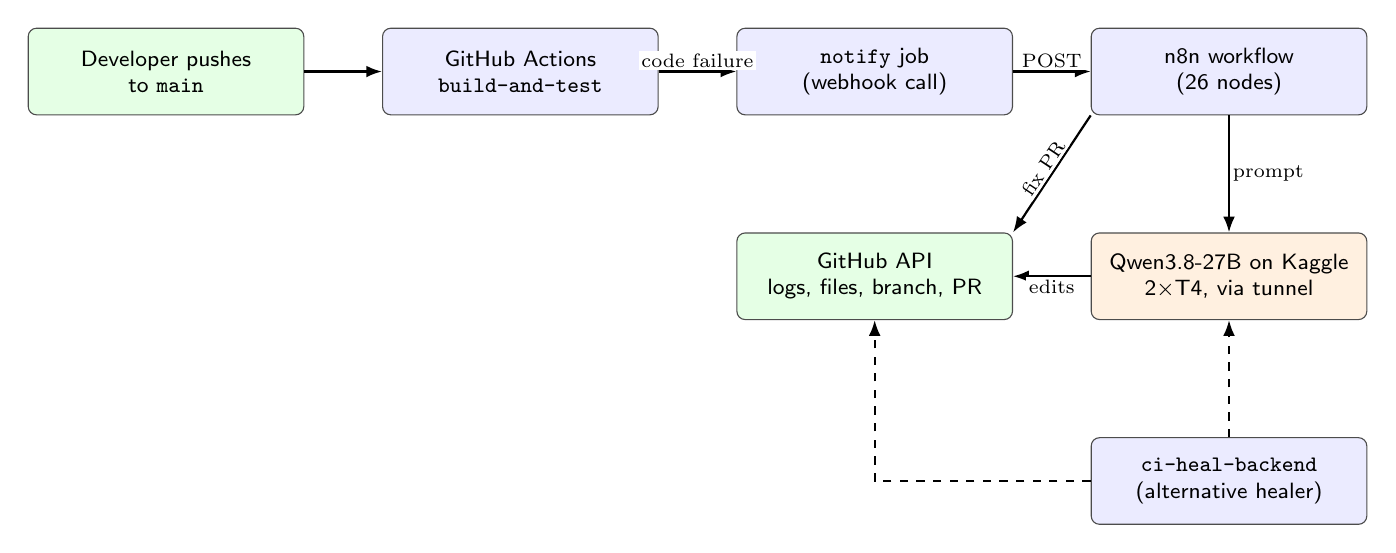
\begin{tikzpicture}[every node/.style={font=\sffamily\footnotesize},
    box/.style={rectangle, rounded corners=3pt, draw=black!70, fill=blue!8, minimum width=3.5cm, minimum height=1.1cm, align=center},
    gbox/.style={box, fill=green!10}, rbox/.style={box, fill=orange!12}]
  \node[gbox] (push) at (0,0)     {Developer pushes\\to \texttt{main}};
  \node[box]  (ci)   at (4.5,0)   {GitHub Actions\\\texttt{build-and-test}};
  \node[box]  (note) at (9.0,0)   {\texttt{notify} job\\(webhook call)};
  \node[box]  (n8n)  at (13.5,0)  {n8n workflow\\(26 nodes)};
  \node[gbox] (api)  at (9.0,-2.6) {GitHub API\\logs, files, branch, PR};
  \node[rbox] (model) at (13.5,-2.6) {Qwen3.8-27B on Kaggle\\2$\times$T4, via tunnel};
  \node[box]  (back) at (13.5,-5.2) {\texttt{ci-heal-backend}\\(alternative healer)};
  \draw[flow] (push) -- (ci);
  \draw[flow] (ci) -- node[lbl, above]{code failure} (note);
  \draw[flow] (note) -- node[lbl, above]{POST} (n8n);
  \draw[flow] (n8n.south) -- node[lbl, right]{prompt} (model.north);
  \draw[flow] (model.west) -- node[lbl, below]{edits} (api.east);
  \draw[flow] (n8n.south west) -- node[lbl, above, sloped]{fix PR} (api.north east);
  \draw[flow, dashed] (back.north) -- (model.south);
  \draw[flow, dashed] (back.west) -| (api.south);
\end{tikzpicture}
\caption{Components of the system and the path of one heal. The dashed arrows show the second healer, which uses the same model endpoint and the same GitHub API.}
\label{fig:architecture}
\end{figure}


The system has six parts. Two of them (the CI workflow and the n8n workflow) take part in every heal, one (the model endpoint) is shared by everything, and the rest are an alternative healer and support tools.

\begingroup\small
\begin{longtable}{>{\raggedright\arraybackslash}p{0.223\dimexpr\linewidth-6\tabcolsep\relax}>{\raggedright\arraybackslash}p{0.345\dimexpr\linewidth-6\tabcolsep\relax}>{\raggedright\arraybackslash}p{0.432\dimexpr\linewidth-6\tabcolsep\relax}}
\toprule
\textbf{Component} & \textbf{What it owns} & \textbf{Where it lives} \\
\midrule
\endhead
\bottomrule
\endfoot
\endlastfoot
GitHub Actions workflow & Runs the tests, decides whether a failure is a code bug, counts heal attempts, calls the healer & \texttt{.\allowbreak{}github/\allowbreak{}workflows/\allowbreak{}demo-\allowbreak{}ci.\allowbreak{}yml} \\
n8n workflow & Collects the evidence, asks the model, applies the edits, opens or updates the fix pull request, reports failures & \texttt{n8n/\allowbreak{}self\_\allowbreak{}healing\_\allowbreak{}pipeline.\allowbreak{}json} (26 nodes, generated by \texttt{tools/\allowbreak{}gen\_\allowbreak{}n8n.\allowbreak{}py}) \\
Kaggle endpoint & Serves Qwen3.8-27B over an OpenAI-style chat API on two T4 GPUs, behind a Cloudflare quick tunnel & \texttt{kaggle/\allowbreak{}endpoint/\allowbreak{}deploy\_\allowbreak{}src.\allowbreak{}py} \\
ci-heal-backend & The alternative healer: a FastAPI service that classifies a failed run, then retries it, opens a fix PR or opens an issue & \texttt{ci-\allowbreak{}heal-\allowbreak{}backend/\allowbreak{}} \\
Launcher scripts & Double-click start and stop scripts for the model, n8n and the backend & \texttt{launcher/\allowbreak{}} \\
Evaluation harness & Bug cases, scorers, unit tests and a real-n8n rig that produced the measurements used in this report & \texttt{eval/\allowbreak{}}, \texttt{tools/\allowbreak{}tests/\allowbreak{}}, \texttt{tools/\allowbreak{}n8n\_\allowbreak{}rig/\allowbreak{}}, \texttt{run\_\allowbreak{}tests.\allowbreak{}py} \\
\bottomrule
\caption{Components}\label{tab:04-1}\\
\end{longtable}
\endgroup

(source: README.md, "Repository layout"; docs/\allowbreak{}architecture/\allowbreak{}n8n-workflow.md; docs/\allowbreak{}architecture/\allowbreak{}kaggle-endpoint.md)

The JSON of the n8n workflow is never edited by hand. \texttt{tools/\allowbreak{}gen\_\allowbreak{}n8n.\allowbreak{}py} writes it, and the bodies of its Code nodes are plain files in \texttt{tools/\allowbreak{}nodes/\allowbreak{}}. Running \texttt{python tools/\allowbreak{}gen\_\allowbreak{}n8n.\allowbreak{}py -\allowbreak{}-\allowbreak{}check} regenerates the file in memory and compares it byte for byte with the shipped copy (source: docs/\allowbreak{}architecture/\allowbreak{}n8n-workflow.md, checked against the node list in n8n/\allowbreak{}self\_\allowbreak{}healing\_\allowbreak{}pipeline.json).

The Kaggle endpoint runs as a script kernel. At boot it unpacks a prebuilt \texttt{llama-\allowbreak{}server}, downloads the GGUF model file, tries context sizes from 131072 downward until one boots, starts a Cloudflare quick tunnel and prints the public address (source: docs/\allowbreak{}architecture/\allowbreak{}kaggle-endpoint.md, describing kaggle/\allowbreak{}endpoint/\allowbreak{}deploy\_\allowbreak{}src.py). The script keeps serving for a 1.5 hour window and then ends by itself.

The launcher is a convenience layer. \texttt{1\_\allowbreak{}start\_\allowbreak{}model\_\allowbreak{}on\_\allowbreak{}kaggle.\allowbreak{}bat} checks the kernel status, builds and pushes the kernel, watches the boot log until the tunnel address appears, and then posts that address to the n8n workflow (source: launcher/\allowbreak{}README.md).

The evaluation harness matters for the architecture because the Code nodes can run outside n8n. \texttt{run\_\allowbreak{}tests.\allowbreak{}py} runs the node suites in \texttt{tools/\allowbreak{}tests/\allowbreak{}}, the eval scorer self-test and the generator check, with no GPU and no writes to GitHub. With \texttt{-\allowbreak{}-\allowbreak{}rig} it also runs a real n8n 1.x engine against mock GitHub hosts (source: run\_\allowbreak{}tests.py, docstring).

\section{Data flow of one heal}

\begin{figure}[!htbp]
\centering
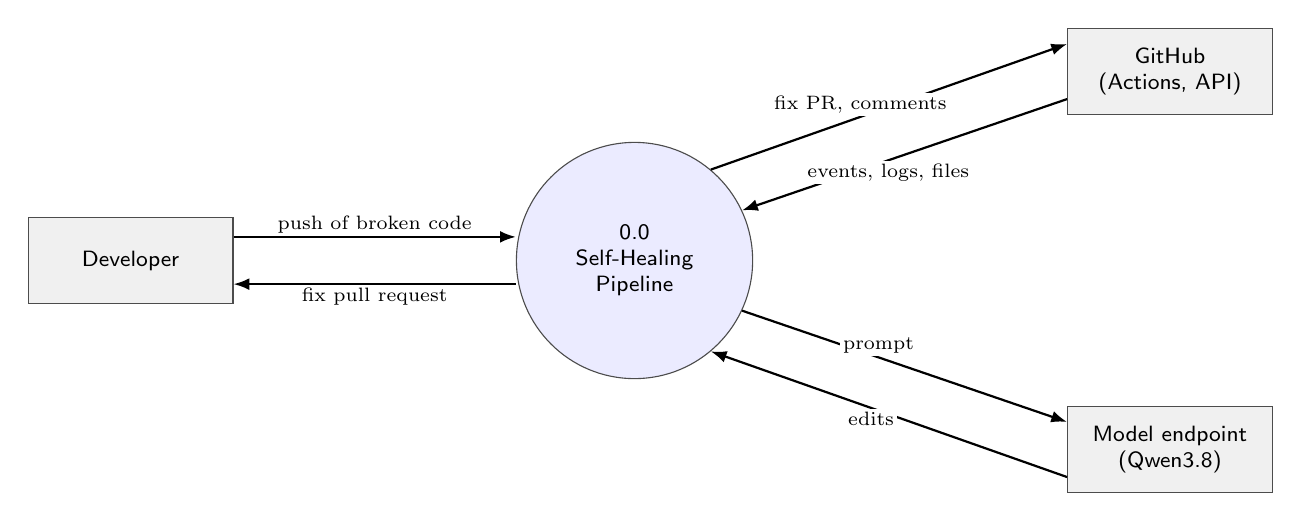
\begin{tikzpicture}[every node/.style={font=\sffamily\footnotesize}]
  \node[ext] (dev) at (0,0) {Developer};
  \node[dfdproc, minimum size=3cm] (core) at (6.4,0) {0.0\\Self-Healing\\Pipeline};
  \node[ext] (gh) at (13.2,2.4) {GitHub\\(Actions, API)};
  \node[ext] (llm) at (13.2,-2.4) {Model endpoint\\(Qwen3.8)};
  \draw[flow] ([yshift=0.3cm]dev.east) -- node[lbl, above]{push of broken code} ([yshift=0.3cm]dev.east -| core.west);
  \draw[flow] ([yshift=-0.3cm]dev.east -| core.west) -- node[lbl, below]{fix pull request} ([yshift=-0.3cm]dev.east);
  \draw[flow] (core.50) -- node[lbl, above, pos=0.42]{fix PR, comments} ([yshift=0.35cm]gh.west);
  \draw[flow] ([yshift=-0.35cm]gh.west) -- node[lbl, below, pos=0.55]{events, logs, files} (core.25);
  \draw[flow] (core.-25) -- node[lbl, above, pos=0.42]{prompt} ([yshift=0.35cm]llm.west);
  \draw[flow] ([yshift=-0.35cm]llm.west) -- node[lbl, below, pos=0.55]{edits} (core.-50);
\end{tikzpicture}
\caption{Level 0 data flow diagram: the whole pipeline as one process with its three external actors.}
\label{fig:dfd0}
\end{figure}

\begin{figure}[!htbp]
\centering
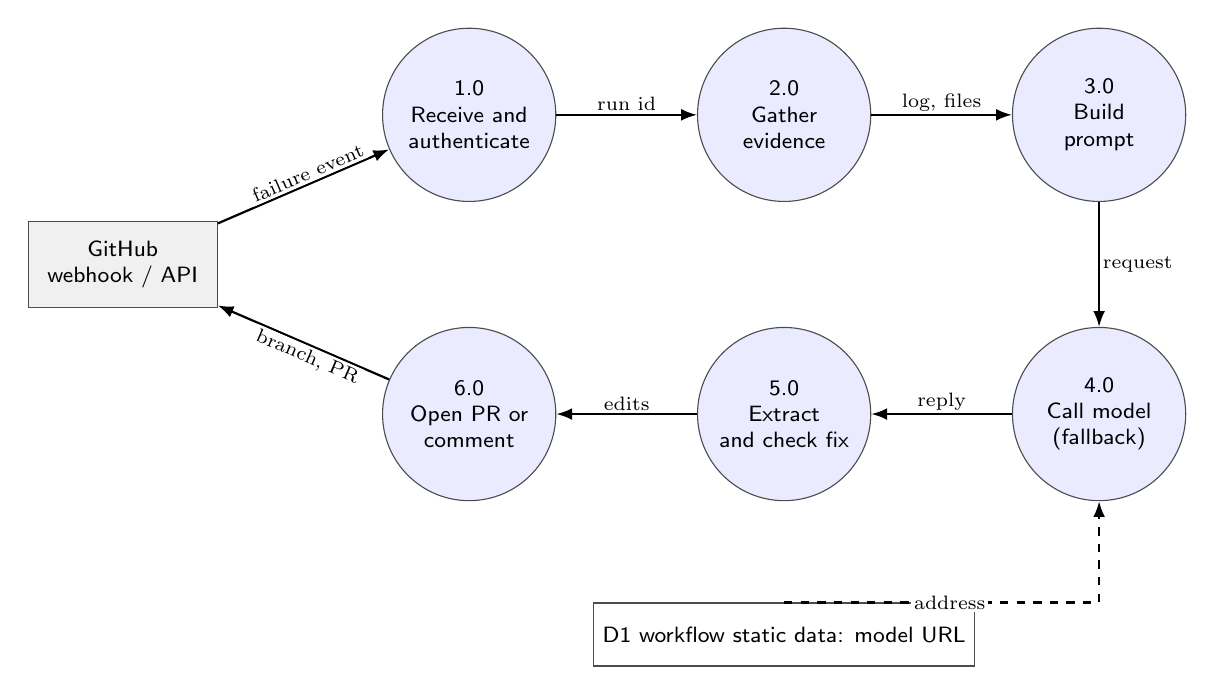
\begin{tikzpicture}[every node/.style={font=\sffamily\scriptsize}]
  \node[ext, minimum width=2.4cm] (gh) at (-0.4,0.3) {GitHub\\webhook / API};
  \node[dfdproc, minimum size=2.2cm] (p1) at (4.0,2.2)  {1.0\\Receive and\\authenticate};
  \node[dfdproc, minimum size=2.2cm] (p2) at (8.0,2.2)  {2.0\\Gather\\evidence};
  \node[dfdproc, minimum size=2.2cm] (p3) at (12.0,2.2) {3.0\\Build\\prompt};
  \node[dfdproc, minimum size=2.2cm] (p4) at (12.0,-1.6) {4.0\\Call model\\(fallback)};
  \node[dfdproc, minimum size=2.2cm] (p5) at (8.0,-1.6) {5.0\\Extract\\and check fix};
  \node[dfdproc, minimum size=2.2cm] (p6) at (4.0,-1.6) {6.0\\Open PR or\\comment};
  \node[store] (d1) at (8.0,-4.4) {D1  workflow static data: model URL};
  \draw[flow] (gh) -- node[lbl, above, sloped, pos=0.55]{failure event} (p1);
  \draw[flow] (p1) -- node[lbl, above]{run id} (p2);
  \draw[flow] (p2) -- node[lbl, above]{log, files} (p3);
  \draw[flow] (p3) -- node[lbl, right]{request} (p4);
  \draw[flow] (p4) -- node[lbl, above]{reply} (p5);
  \draw[flow] (p5) -- node[lbl, above]{edits} (p6);
  \draw[flow] (p6) -- node[lbl, below, sloped, pos=0.45]{branch, PR} (gh);
  \draw[flow, dashed] (d1.north) -| node[lbl, pos=0.2, right]{address} (p4.south);
\end{tikzpicture}
\caption{Level 1 data flow diagram: the six sub-processes of the n8n healer and the one data store.}
\label{fig:dfd1}
\end{figure}


The steps below follow a first-time heal from the push to the open pull request.

\begin{enumerate}[leftmargin=*, itemsep=2pt]
\item A developer pushes a commit that changes \texttt{demo-\allowbreak{}app/\allowbreak{}} to \texttt{main}, and the workflow starts (source: .github/\allowbreak{}workflows/\allowbreak{}demo-ci.yml, \texttt{on.\allowbreak{}push}).
\item The \texttt{build-\allowbreak{}and-\allowbreak{}test} job runs \texttt{npm test} and turns the exit code into \texttt{failure\_\allowbreak{}kind}: \texttt{none} for 0, \texttt{infra} for 75 and \texttt{code} for anything else (source: .github/\allowbreak{}workflows/\allowbreak{}demo-ci.yml, step "Run tests").
\item The \texttt{notify-\allowbreak{}n8n-\allowbreak{}on-\allowbreak{}failure} job runs only when \texttt{failure\_\allowbreak{}kind} is \texttt{code} and the event is a push or the branch starts with \texttt{ai-\allowbreak{}fix-\allowbreak{}}. On a push it sets \texttt{attempt=0} and \texttt{action=heal}.
\item The notify job POSTs a JSON body to the n8n webhook. The fields are in the table below.
\item n8n answers GitHub at once (response mode \texttt{onReceived}) and keeps working (source: n8n/\allowbreak{}self\_\allowbreak{}healing\_\allowbreak{}pipeline.json, node "GitHub Failure Webhook").
\item n8n lists the run's jobs, finds the failed one, downloads its log, lists the commit's changed files and picks up to 3 candidate files (source: tools/\allowbreak{}nodes/\allowbreak{}pick\_\allowbreak{}candidate\_\allowbreak{}files.js, \texttt{MAX = 3}, as described in docs/\allowbreak{}architecture/\allowbreak{}n8n-workflow.md).
\item n8n builds one prompt from the failure details, the trimmed log and the source of each candidate file. For a first heal it sets \texttt{enable\_\allowbreak{}thinking} to false.
\item n8n sends the request to the model address it has stored. The reply comes back as a stream of server-sent events.
\item n8n rebuilds the reply, reads the JSON object, applies the SEARCH/\allowbreak{}REPLACE blocks to the file the model named and checks that the result parses.
\item n8n creates the \texttt{ai-\allowbreak{}fix-\allowbreak{}.\allowbreak{}.\allowbreak{}.\allowbreak{}} branch from the failing commit, pushes the patched file with a commit message that ends in \texttt{Heal-\allowbreak{}Attempt:\allowbreak{} 1}, and opens a pull request into the branch that failed (source: tools/\allowbreak{}nodes/\allowbreak{}extract\_\allowbreak{}ai\_\allowbreak{}response.js; n8n/\allowbreak{}self\_\allowbreak{}healing\_\allowbreak{}pipeline.json, node "Open Pull Request").
\item The workflow also triggers on pull requests into \texttt{main}, so the fix PR gets its own CI run. If that run fails with a code failure, the notify job runs again with \texttt{attempt=1} and the loop continues (Chapters 5 and 6).
\end{enumerate}

The webhook body has these fields (source: .github/\allowbreak{}workflows/\allowbreak{}demo-ci.yml, step "Trigger n8n webhook").

\begingroup\small
\begin{longtable}{>{\raggedright\arraybackslash}p{0.207\dimexpr\linewidth-6\tabcolsep\relax}>{\raggedright\arraybackslash}p{0.397\dimexpr\linewidth-6\tabcolsep\relax}>{\raggedright\arraybackslash}p{0.397\dimexpr\linewidth-6\tabcolsep\relax}}
\toprule
\textbf{Field} & \textbf{Value} & \textbf{Used for} \\
\midrule
\endhead
\bottomrule
\endfoot
\endlastfoot
\texttt{run\_\allowbreak{}id} & \texttt{github.\allowbreak{}run\_\allowbreak{}id} & Listing the jobs of the failed run \\
\texttt{repo} & \texttt{owner/\allowbreak{}name} & Every GitHub API URL \\
\texttt{branch} & The pushed branch, or the head branch of the fix PR & Base of the new PR; retry detection by the \texttt{ai-\allowbreak{}fix-\allowbreak{}} prefix \\
\texttt{commit} & The pushed commit on a push, the PR head commit on a pull request & Source of file contents; base of the new branch \\
\texttt{actor} & \texttt{github.\allowbreak{}actor} & Shown in the prompt \\
\texttt{failure\_\allowbreak{}kind} & \texttt{code} in practice & A second check inside n8n \\
\texttt{attempt} & \texttt{0} on a push, the \texttt{Heal-\allowbreak{}Attempt} number on a fix PR & Turns thinking on; numbers the next commit \\
\texttt{pr\_\allowbreak{}number} & The PR number on a pull request event & Where a failure comment is posted \\
\bottomrule
\caption{Data flow of one heal}\label{tab:04-2}\\
\end{longtable}
\endgroup

All values are sent as strings inside the JSON. On a push event the expression for \texttt{pr\_\allowbreak{}number} has nothing to read, so it should arrive empty. That is my inference from the expression, not something we observed. \texttt{tools/\allowbreak{}nodes/\allowbreak{}explain\_\allowbreak{}failure.\allowbreak{}js} treats anything that is not all digits as "no PR".

\section{Trust boundaries and secrets}

Four boundaries are crossed during one heal, and each has its own protection.

\begingroup\small
\begin{longtable}{>{\raggedright\arraybackslash}p{0.295\dimexpr\linewidth-4\tabcolsep\relax}>{\raggedright\arraybackslash}p{0.705\dimexpr\linewidth-4\tabcolsep\relax}}
\toprule
\textbf{Boundary} & \textbf{What protects it} \\
\midrule
\endhead
\bottomrule
\endfoot
\endlastfoot
GitHub runner to n8n webhook & A shared secret in the header \texttt{X-\allowbreak{}Webhook-\allowbreak{}Secret}, checked by n8n's header authentication. A wrong or missing secret is rejected before the workflow starts (source: docs/\allowbreak{}architecture/\allowbreak{}n8n-workflow.md) \\
n8n to the GitHub API & A bearer token held in the n8n credential "GitHub PAT", used by nine request nodes (source: docs/\allowbreak{}guides/\allowbreak{}cloud-n8n.md) \\
n8n to the model & A bearer key held in the n8n credential "Qwen3.8 Endpoint Key", checked by \texttt{llama-\allowbreak{}server} through \texttt{-\allowbreak{}-\allowbreak{}api-\allowbreak{}key} \\
n8n to the log storage host & No credential at all, on purpose (see the design decision on redirects) \\
\bottomrule
\caption{Trust boundaries and secrets}\label{tab:04-3}\\
\end{longtable}
\endgroup

The secrets live in these places. No value is printed here.

\begingroup\small
\begin{longtable}{>{\raggedright\arraybackslash}p{0.218\dimexpr\linewidth-4\tabcolsep\relax}>{\raggedright\arraybackslash}p{0.782\dimexpr\linewidth-4\tabcolsep\relax}}
\toprule
\textbf{Secret} & \textbf{Where it lives} \\
\midrule
\endhead
\bottomrule
\endfoot
\endlastfoot
Webhook shared secret & GitHub repository secret \texttt{N8N\_\allowbreak{}WEBHOOK\_\allowbreak{}SECRET}; the n8n credential "N8N Webhook Secret"; the field \texttt{webhook\_\allowbreak{}secret} in \texttt{\%LOCALAPPDATA\%\textbackslash{}selfheal-\allowbreak{}n8n\textbackslash{}secrets.\allowbreak{}json} (source: docs/\allowbreak{}guides/\allowbreak{}cloud-n8n.md) \\
Webhook address & GitHub repository secret \texttt{N8N\_\allowbreak{}WEBHOOK\_\allowbreak{}URL} (source: .github/\allowbreak{}workflows/\allowbreak{}demo-ci.yml) \\
GitHub PAT & The n8n credential "GitHub PAT". For a local n8n, \texttt{tools/\allowbreak{}golive/\allowbreak{}n8n\_\allowbreak{}import.\allowbreak{}py} takes the token from \texttt{gh auth token}, writes it into n8n's credential store and deletes the plaintext import file. On n8n Cloud it is created by hand in the browser (source: docs/\allowbreak{}guides/\allowbreak{}cloud-n8n.md) \\
n8n encryption key & The field \texttt{encryption\_\allowbreak{}key} in \texttt{secrets.\allowbreak{}json}, used by the local n8n (source: tools/\allowbreak{}golive/\allowbreak{}n8n\_\allowbreak{}import.py) \\
Endpoint API key & A constant \texttt{API\_\allowbreak{}KEY} in \texttt{kaggle/\allowbreak{}endpoint/\allowbreak{}deploy\_\allowbreak{}src.\allowbreak{}py}, and the n8n credential "Qwen3.8 Endpoint Key" (source: docs/\allowbreak{}architecture/\allowbreak{}kaggle-endpoint.md, "API key") \\
Current model address & \texttt{\%LOCALAPPDATA\%\textbackslash{}selfheal-\allowbreak{}n8n\textbackslash{}qwen\_\allowbreak{}url.\allowbreak{}txt} on the PC, and the workflow's static data in n8n (source: tools/\allowbreak{}nodes/\allowbreak{}store\_\allowbreak{}model\_\allowbreak{}url.js) \\
Backend secrets & \texttt{ci-\allowbreak{}heal-\allowbreak{}backend/\allowbreak{}.\allowbreak{}env} (\texttt{GITHUB\_\allowbreak{}TOKEN}, \texttt{GITHUB\_\allowbreak{}WEBHOOK\_\allowbreak{}SECRET}, \texttt{N8N\_\allowbreak{}SHARED\_\allowbreak{}TOKEN} and others). \texttt{.\allowbreak{}gitignore} lists \texttt{*.\allowbreak{}env} and \texttt{secrets.\allowbreak{}json} \\
\bottomrule
\caption{Trust boundaries and secrets}\label{tab:04-4}\\
\end{longtable}
\endgroup

The folder \texttt{\%LOCALAPPDATA\%\textbackslash{}selfheal-\allowbreak{}n8n} is outside the repository on purpose. It also holds the local n8n install and database, the tunnel logs and the process ids (source: tools/\allowbreak{}golive/\allowbreak{}up.py, docstring; tools/\allowbreak{}golive/\allowbreak{}exec\_\allowbreak{}stats.py).

Two weak points should be stated plainly. The endpoint key is a fixed string inside a file that is committed to the repository, so anyone with repository access can read it (source: docs/\allowbreak{}architecture/\allowbreak{}kaggle-endpoint.md). And the quick tunnel makes the model server reachable from the internet, so that key is the only thing between a stranger and the GPU.

The JSON of the workflow holds no secrets. \texttt{tools/\allowbreak{}tests/\allowbreak{}test\_\allowbreak{}workflow\_\allowbreak{}structure.\allowbreak{}py} searches it for token prefixes, and the OpenAI node ships with no credential bound (source: docs/\allowbreak{}architecture/\allowbreak{}n8n-workflow.md, "Credentials and variables").

\section{One healer per repository}

The n8n workflow and ci-heal-backend are two separate healers, and a repository should use only one of them. GitHub tells both about the same failed run: n8n through the notify job, the backend through a \texttt{workflow\_\allowbreak{}run} webhook. With both active, each would open its own fix PR for the same bug and the two would compete (source: README.md, "How the parts connect"; launcher/\allowbreak{}README.md).

They also decide differently. The n8n workflow acts only on failures the CI job marked as \texttt{code}, and then always tries a fix. The backend classifies the failure first and then reruns a flaky job, opens a fix PR or opens an issue, depending on its confidence (source: ci-heal-backend/\allowbreak{}README.md). Their attempt counters are separate too: n8n uses the \texttt{Heal-\allowbreak{}Attempt} trailer, while the backend counts fix decisions in its own database (source: ci-heal-backend/\allowbreak{}README.md, Architecture). Neither counter knows about the other.

The backend has an endpoint \texttt{POST /\allowbreak{}webhooks/\allowbreak{}n8n} for failures forwarded from n8n (source: ci-heal-backend/\allowbreak{}README.md). We found no node in the shipped workflow that calls it, so that route is not part of the n8n healer described in this report.

\section{Design decisions}

\subsection{SEARCH/\allowbreak{}REPLACE edits instead of whole files}

The model answers with a JSON object whose \texttt{edits} field holds SEARCH/\allowbreak{}REPLACE blocks. The first version asked for the whole fixed file, which made the model copy nearly all of its input back out. Output tokens cost time on this hardware (the baseline run measured 12.29 tok/\allowbreak{}s), so three formats were measured on 45 calls (source: docs/\allowbreak{}results/\allowbreak{}DIFF\_\allowbreak{}FORMAT\_\allowbreak{}EVAL.md).

\begingroup\small
\begin{longtable}{>{\raggedright\arraybackslash}p{0.358\dimexpr\linewidth-8\tabcolsep\relax}>{\raggedright\arraybackslash}p{0.296\dimexpr\linewidth-8\tabcolsep\relax}>{\raggedright\arraybackslash}p{0.123\dimexpr\linewidth-8\tabcolsep\relax}>{\raggedright\arraybackslash}p{0.222\dimexpr\linewidth-8\tabcolsep\relax}}
\toprule
\textbf{Format} & \textbf{Median completion tokens} & \textbf{Wall time} & \textbf{Applied and parsed} \\
\midrule
\endhead
\bottomrule
\endfoot
\endlastfoot
Whole file & 655 & 56.4 s & 15/\allowbreak{}15 \\
Unified diff & 233 & 23.3 s & 12/\allowbreak{}15 \\
SEARCH/\allowbreak{}REPLACE & 171 & 17.0 s & 15/\allowbreak{}15 \\
\bottomrule
\caption{SEARCH/\allowbreak{}REPLACE edits instead of whole files}\label{tab:04-5}\\
\end{longtable}
\endgroup

(source: docs/\allowbreak{}results/\allowbreak{}DIFF\_\allowbreak{}FORMAT\_\allowbreak{}EVAL.md, "Results")

The unified diff lost on correctness as well as speed. In one scenario the model wrote a patch whose header claimed an added line while the only added line was empty, and a tolerant \texttt{-\allowbreak{}-\allowbreak{}recount} retry applied it as a no-op that still did not parse (source: same file). SEARCH/\allowbreak{}REPLACE avoids this because every block must match the current file exactly once, or the whole fix is rejected. The rule is enforced in \texttt{tools/\allowbreak{}nodes/\allowbreak{}extract\_\allowbreak{}ai\_\allowbreak{}response.\allowbreak{}js}. In the first live round the median model phase fell from about 57 s to 11.4 s (source: docs/\allowbreak{}results/\allowbreak{}GOLIVE\_\allowbreak{}RESULTS.md).

\subsection{Streamed model calls}

The model sits behind a Cloudflare quick tunnel, which cuts a request when the origin stays silent for 120 seconds. A thinking retry once died that way, with HTTP 524 at 125.9 s. A proof run sent the same long request through the same tunnel twice: without streaming it failed with 524 at 125.9 s, and with streaming it finished with HTTP 200 after 166.5 s (source: docs/\allowbreak{}results/\allowbreak{}GOLIVE\_\allowbreak{}RESULTS.md, Round 5). So the request sets \texttt{stream:\allowbreak{} true}, and a Code node called "Assemble Model Reply" rebuilds the ordinary completion from the event stream. A stream that ends with neither \texttt{[DONE]} nor a finish reason counts as cut off and as a failed call (source: tools/\allowbreak{}nodes/\allowbreak{}assemble\_\allowbreak{}model\_\allowbreak{}reply.js, as described in docs/\allowbreak{}architecture/\allowbreak{}n8n-workflow.md).

\subsection{Thinking off first, on for retries}

With thinking off, the first pass healed 15/\allowbreak{}15 control cases and 12/\allowbreak{}18 hard cases, with a median wall time of 9.1 s. With thinking on and a 1024-token budget it healed 18/\allowbreak{}18 hard cases, including two that no earlier configuration had fixed, but the median rose to 36.8 s (source: docs/\allowbreak{}results/\allowbreak{}SHIPPED\_\allowbreak{}QUALITY\_\allowbreak{}EVAL.md, arms B and C). Always thinking would add about 28 s to every heal, so the workflow turns it on only after CI has rejected the fast fix. \texttt{Build AI Prompt} sets \texttt{enable\_\allowbreak{}thinking} to the value of \texttt{isRetry} (source: tools/\allowbreak{}nodes/\allowbreak{}build\_\allowbreak{}ai\_\allowbreak{}prompt.js). The server itself defaults to thinking off, because the backend can only switch it on per request (source: docs/\allowbreak{}architecture/\allowbreak{}kaggle-endpoint.md, "Why thinking is off by default").

The price is that a hard bug needs one more CI cycle. In the live retry rounds, \texttt{multi\_\allowbreak{}hunk} turned green on attempt 2 in 143 to 161 s, and \texttt{callback\_\allowbreak{}arity}, which failed in earlier rounds, turned green on attempt 3 in 249 s (source: docs/\allowbreak{}results/\allowbreak{}GOLIVE\_\allowbreak{}RESULTS.md, Rounds 3 and 5).

\subsection{The failure\_\allowbreak{}kind gate}

An infrastructure problem, such as a port that is already in use, has nothing to fix in the source. If the model were asked anyway, it would invent a patch. The demo tests therefore exit with 75 for environment problems and with 1 for code failures, and the workflow maps these to \texttt{infra} and \texttt{code} (source: demo-app/\allowbreak{}test.js, header comment). We checked on this machine that \texttt{npm test} exits with 75 when port 5000 is already taken. The gate exists twice: the notify job runs only for \texttt{code}, and \texttt{Build AI Prompt} throws \texttt{Refusing to run} for any other non-empty \texttt{failure\_\allowbreak{}kind}, because the webhook is a public address that anyone could post to (source: tools/\allowbreak{}nodes/\allowbreak{}build\_\allowbreak{}ai\_\allowbreak{}prompt.js).

\subsection{Log redirect handling}

GitHub answers a job-log request with a 302 redirect to a signed address on another host. The first design let one HTTP node follow the redirect, assuming the client drops the \texttt{Authorization} header when the host changes. The real-n8n rig showed that its mock storage host received the bearer token. The fix uses two nodes. "Fetch Failed Job Log" does not follow redirects and returns the \texttt{Location}, and "Download Job Log" fetches that address with no credential. The rig now asserts that the token reached the API host and did not reach the storage host (source: docs/\allowbreak{}results/\allowbreak{}GOLIVE\_\allowbreak{}RESULTS.md, Round 2, "Two defects the verification caught"; n8n/\allowbreak{}self\_\allowbreak{}healing\_\allowbreak{}pipeline.json).

\subsection{Model address stored through a webhook}

The quick tunnel gets a new address on every Kaggle boot, so the address has to be delivered again each time. Earlier the update went through the n8n API (source: git commit 4833c44, whose message says it switched from the API to a webhook). On an n8n Cloud trial the REST API is switched off (source: docs/\allowbreak{}guides/\allowbreak{}cloud-n8n.md, "Trial limits"), so the workflow got a second webhook, "Set Model URL", protected by the same shared secret, and the launcher posts the new address to it. The node "Store Model URL" accepts only an address of the form \texttt{https:\allowbreak{}/\allowbreak{}/\allowbreak{}\textless{}name\textgreater{}.\allowbreak{}trycloudflare.\allowbreak{}com} and saves it in the workflow's static data, so a mistyped or hostile value is refused (source: tools/\allowbreak{}nodes/\allowbreak{}store\_\allowbreak{}model\_\allowbreak{}url.js). "Get Model URL" reads the stored address before each model call and falls back to the variable \texttt{QWEN\_\allowbreak{}BASE\_\allowbreak{}URL} (source: tools/\allowbreak{}nodes/\allowbreak{}get\_\allowbreak{}model\_\allowbreak{}url.js).

\subsection{The attempt counter lives in the commit}

The cap on retries has to survive a re-run of the workflow and a restart of n8n. For that reason the count is a \texttt{Heal-\allowbreak{}Attempt:\allowbreak{} N} line in the message of every commit the healer pushes, and the notify job reads it from the head commit of the fix PR (source: .github/\allowbreak{}workflows/\allowbreak{}demo-ci.yml, comment on \texttt{MAX\_\allowbreak{}ATTEMPTS}). The cap is enforced in the notify job only. The n8n workflow does not check it (source: docs/\allowbreak{}architecture/\allowbreak{}n8n-workflow.md, "The retry loop").

% GENERATED by build_chapters.py; edit docs/report/chapters, not this file

\chapter{GitHub Actions and the Notify Job}

Everything on the GitHub side is one workflow file, \texttt{.\allowbreak{}github/\allowbreak{}workflows/\allowbreak{}demo-\allowbreak{}ci.\allowbreak{}yml}, named "Demo CI", plus the small Node application it tests in \texttt{demo-\allowbreak{}app/\allowbreak{}}. The workflow does two jobs: it tests the code, and when the tests fail because of a code bug it wakes the healer. This chapter goes through the file from top to bottom.

\section{Triggers}

\begin{lstlisting}
on:
  push:
    branches:
      - main
    paths: ["demo-app/**"]
  pull_request:
    branches:
      - main
    paths: ["demo-app/**"]
\end{lstlisting}

(source: .github/\allowbreak{}workflows/\allowbreak{}demo-ci.yml)

The workflow starts in two cases. A push to \texttt{main} starts it, and so does a pull request that targets \texttt{main}. In both cases the changed files must include something under \texttt{demo-\allowbreak{}app/\allowbreak{}}. The path filter keeps documentation commits, report files and the rest of the repository from running the tests.

The path filter has a side effect. A change that touches only files outside \texttt{demo-\allowbreak{}app/\allowbreak{}} does not start CI at all, so a failing test could not be reported for it. That does not matter for the demo, whose bugs live in the app, but it would matter for a real repository, where the filter would have to cover every folder that can break the build.

The \texttt{pull\_\allowbreak{}request} trigger was added so that the fix pull requests opened by the healer are tested too. The reason is in the last section of this chapter.

\section{Jobs}

There are two jobs, \texttt{build-\allowbreak{}and-\allowbreak{}test} and \texttt{notify-\allowbreak{}n8n-\allowbreak{}on-\allowbreak{}failure}. The second one names the first in \texttt{needs}, so it waits for it and can read its outputs. Both run on \texttt{ubuntu-\allowbreak{}latest}.

\section{The build-and-test job}

The job's default working directory is \texttt{demo-\allowbreak{}app}. Its steps are as follows (source: .github/\allowbreak{}workflows/\allowbreak{}demo-ci.yml).

\begin{enumerate}[leftmargin=*, itemsep=2pt]
\item Check out the code with \texttt{actions/\allowbreak{}checkout@v4}.
\item Install Node.js 20 with \texttt{actions/\allowbreak{}setup-\allowbreak{}node@v4}.
\item Run \texttt{npm install}.
\item Run the tests (step id \texttt{tests}) and classify the result.
\item Run \texttt{npm run build -\allowbreak{}-\allowbreak{}if-\allowbreak{}present}.
\end{enumerate}

The fourth step is the one that matters for healing. It runs \texttt{npm test} with \texttt{set +e}, so the script survives a failure and can inspect the exit code:

\begin{lstlisting}
- name: Run tests
  id: tests
  run: |
    set +e
    npm test
    code=$?
    set -e
    if [ "$code" -eq 0 ]; then
      kind=none
    elif [ "$code" -eq 75 ]; then
      kind=infra
    else
      kind=code
    fi
    echo "failure_kind=$kind" >> "$GITHUB_OUTPUT"
    exit "$code"
\end{lstlisting}

(shortened; source: .github/\allowbreak{}workflows/\allowbreak{}demo-ci.yml, step "Run tests")

The result is published as a job output, \texttt{failure\_\allowbreak{}kind}, which the second job reads. The step then exits with the original code, so the job still turns red when the tests fail. The exit code 75 is \texttt{EX\_\allowbreak{}TEMPFAIL}, the conventional "try again later" code (source: demo-app/\allowbreak{}test.js, header comment).

Two situations leave \texttt{failure\_\allowbreak{}kind} without the value \texttt{code}, and both are consequences of how the step is written, not of anything the workflow says. If \texttt{npm install} fails, the tests step never runs, so the output is empty. If the tests pass and only the build step fails, the output is \texttt{none}. Either way the notify job's condition is false and the healer is not called. The first case is intended, since a failed install is an environment matter. The second is a gap: a build failure after passing tests is not healed. In this demo the build script only runs \texttt{node index.\allowbreak{}js}, which prints one line (source: demo-app/\allowbreak{}package.json, demo-app/\allowbreak{}index.js).

\section{The notify job}

\subsection{When it runs}

\begin{lstlisting}
if: >-
  failure() && needs.build-and-test.outputs.failure_kind == 'code' &&
  (github.event_name == 'push' || startsWith(github.head_ref, 'ai-fix-'))
permissions:
  contents: read
  pull-requests: write
  issues: write
env:
  MAX_ATTEMPTS: 3
\end{lstlisting}

(source: .github/\allowbreak{}workflows/\allowbreak{}demo-ci.yml)

The condition has three parts. \texttt{failure()} makes the job run only when an earlier job failed. The \texttt{failure\_\allowbreak{}kind} check stops it for infrastructure problems: the file's own comment says that \texttt{failure()} alone would also fire for a bound port, DNS or a full runner disk, and that the model would then invent a patch for a problem that is not in the source. The third part limits the event. A push to \texttt{main} always qualifies. A pull request qualifies only when its head branch starts with \texttt{ai-\allowbreak{}fix-\allowbreak{}}, which is the prefix the healer uses. A human's pull request therefore never wakes the healer.

The job asks for \texttt{pull-\allowbreak{}requests:\allowbreak{} write} and \texttt{issues:\allowbreak{} write}. The file does not say why, but its last step comments on a pull request, which is the likely reason.

\texttt{MAX\_\allowbreak{}ATTEMPTS} is 3. That is the total number of model attempts per heal PR: the first heal plus two retries (source: comment in .github/\allowbreak{}workflows/\allowbreak{}demo-ci.yml).

\subsection{Step 1: decide}

The step with id \texttt{decide} produces four outputs: \texttt{branch}, \texttt{commit}, \texttt{attempt} and \texttt{action}.

On a push the answer is fixed: the branch is \texttt{GITHUB\_\allowbreak{}REF\_\allowbreak{}NAME}, the commit is \texttt{GITHUB\_\allowbreak{}SHA}, \texttt{attempt} is 0 and \texttt{action} is \texttt{heal}.

On a pull request the step looks at the head commit of the PR, not at \texttt{github.\allowbreak{}sha}. For a pull request event, \texttt{github.\allowbreak{}sha} points at a merge commit that GitHub makes, and that commit does not carry the healer's message. The step fetches the head commit's message through the API and reads the trailer:

\begin{lstlisting}
attempt=$(printf '%s\n' "$msg" | sed -n 's/^Heal-Attempt: *\([0-9][0-9]*\) *$/\1/p' | tail -n 1)
\end{lstlisting}

(source: .github/\allowbreak{}workflows/\allowbreak{}demo-ci.yml, step "Decide")

The \texttt{Heal-\allowbreak{}Attempt:\allowbreak{} N} line is added by the healer to every commit it pushes, and the first heal is numbered 1 (source: tools/\allowbreak{}nodes/\allowbreak{}extract\_\allowbreak{}ai\_\allowbreak{}response.js). The step then picks one of three actions:

\begingroup\small
\begin{longtable}{>{\raggedright\arraybackslash}p{0.311\dimexpr\linewidth-6\tabcolsep\relax}>{\raggedright\arraybackslash}p{0.156\dimexpr\linewidth-6\tabcolsep\relax}>{\raggedright\arraybackslash}p{0.533\dimexpr\linewidth-6\tabcolsep\relax}}
\toprule
\textbf{Trailer found} & \textbf{Action} & \textbf{Meaning} \\
\midrule
\endhead
\bottomrule
\endfoot
\endlastfoot
None & \texttt{none} & A human pushed to the heal branch and owns it now. The step prints a notice and nothing else happens \\
N is at least \texttt{MAX\_\allowbreak{}ATTEMPTS} & \texttt{giveup} & The cap is reached \\
Otherwise & \texttt{heal} & Call the healer again with \texttt{attempt=N} \\
\bottomrule
\caption{Step 1: decide}\label{tab:05-1}\\
\end{longtable}
\endgroup

With the cap at 3, the commit numbering works out as follows. The first heal commit carries \texttt{Heal-\allowbreak{}Attempt:\allowbreak{} 1}. When CI fails on it, the notify job reads 1, which is below 3, and calls the healer, which pushes a commit marked 2. A second failure reads 2 and produces a commit marked 3. A third failure reads 3 and gives up. That is three model attempts in total.

The counter sits in the commit message, so re-running the workflow cannot reset it (source: comment in .github/\allowbreak{}workflows/\allowbreak{}demo-ci.yml).

\subsection{Step 2: trigger the webhook}

This step runs when \texttt{action} is \texttt{heal}. It posts to the address in the repository secret \texttt{N8N\_\allowbreak{}WEBHOOK\_\allowbreak{}URL}, with the shared secret in the header \texttt{X-\allowbreak{}Webhook-\allowbreak{}Secret}:

\begin{lstlisting}
curl -sS --fail --max-time 20 -X POST "${{ secrets.N8N_WEBHOOK_URL }}" \
  -H "Content-Type: application/json" \
  -H "X-Webhook-Secret: ${{ secrets.N8N_WEBHOOK_SECRET }}" \
  -d '{ "run_id": "...", "repo": "...", "branch": "...", "commit": "...",
        "actor": "...", "failure_kind": "...", "attempt": "...",
        "pr_number": "..." }' \
  || echo "::warning::n8n webhook unreachable - heal not triggered"
\end{lstlisting}

(shortened; each value is a \texttt{\$\{\{ \}\}} expression in the real file; source: .github/\allowbreak{}workflows/\allowbreak{}demo-ci.yml)

The fields and what n8n does with them are listed in Chapter 4. Three details stand out. The request has a 20 second limit (\texttt{-\allowbreak{}-\allowbreak{}max-\allowbreak{}time 20}). \texttt{-\allowbreak{}-\allowbreak{}fail} makes curl report an HTTP error as a failure. And the trailing \texttt{\textbar{}\textbar{} echo ":\allowbreak{}:\allowbreak{}warning:\allowbreak{}:\allowbreak{}.\allowbreak{}.\allowbreak{}.\allowbreak{}"} turns any failure of the call into a warning annotation, so the step itself still succeeds.

The warning exists because the webhook address is a tunnel that is only up while the healer is deployed. Without the fallback, a stopped healer would turn every broken commit red a second time, for a reason unrelated to the commit. The go-live notes record a test with the healer down: the build job failed and the notify job ended as success, with the warning shown in the annotations (source: docs/\allowbreak{}results/\allowbreak{}GOLIVE\_\allowbreak{}RESULTS.md, Round 2).

\subsection{Step 3: give up at the cap}

When \texttt{action} is \texttt{giveup}, the last step posts a comment on the pull request with \texttt{gh pr comment}. The text says how many attempts were made, that the pipeline has stopped and that the case needs a human (source: .github/\allowbreak{}workflows/\allowbreak{}demo-ci.yml). This is the only place where the cap is enforced. The n8n workflow does not check it (source: docs/\allowbreak{}architecture/\allowbreak{}n8n-workflow.md).

\section{The demo application}

The application is small on purpose. It stands in for a real project, and the pipeline would work the same way on one (source: demo-app/\allowbreak{}index.js, comment).

\begingroup\small
\begin{longtable}{>{\raggedright\arraybackslash}p{0.510\dimexpr\linewidth-4\tabcolsep\relax}>{\raggedright\arraybackslash}p{0.490\dimexpr\linewidth-4\tabcolsep\relax}}
\toprule
\textbf{File} & \textbf{Role} \\
\midrule
\endhead
\bottomrule
\endfoot
\endlastfoot
\texttt{demo-\allowbreak{}app/\allowbreak{}index.\allowbreak{}js} & Entry point. It prints one line and nothing else \\
\texttt{demo-\allowbreak{}app/\allowbreak{}src/\allowbreak{}app.\allowbreak{}js} & An Express app with three routes: \texttt{GET /\allowbreak{}health}, \texttt{GET /\allowbreak{}greet/\allowbreak{}:\allowbreak{}name} and \texttt{GET /\allowbreak{}sum?a=\&b=} \\
\texttt{demo-\allowbreak{}app/\allowbreak{}src/\allowbreak{}format.\allowbreak{}js} & Two helpers, \texttt{formatGreeting} and \texttt{formatSum}, used by the routes \\
\texttt{demo-\allowbreak{}app/\allowbreak{}test.\allowbreak{}js} & The smoke test: starts its own Express server on \texttt{PORT} (default 5000), requests \texttt{/\allowbreak{}} and expects status 200 \\
\texttt{demo-\allowbreak{}app/\allowbreak{}test/\allowbreak{}api.\allowbreak{}test.\allowbreak{}js} & The API test: loads \texttt{src/\allowbreak{}app.\allowbreak{}js}, listens on \texttt{API\_\allowbreak{}PORT} (default 5055) and checks four requests \\
\texttt{demo-\allowbreak{}app/\allowbreak{}package.\allowbreak{}json} & The one dependency is \texttt{express} \texttt{\textasciicircum{}4.\allowbreak{}19.\allowbreak{}2}. The \texttt{test} script is \texttt{node test.\allowbreak{}js \&\& node test/\allowbreak{}api.\allowbreak{}test.\allowbreak{}js} \\
\bottomrule
\caption{The demo application}\label{tab:05-2}\\
\end{longtable}
\endgroup

(source: the files listed)

The four API checks are \texttt{/\allowbreak{}health} returning \texttt{\{"status":\allowbreak{}"ok"\}}, \texttt{/\allowbreak{}greet/\allowbreak{}Ada} returning \texttt{Hello, Ada!}, \texttt{/\allowbreak{}sum?a=2\&b=3} returning a sum of 5, and \texttt{/\allowbreak{}sum?a=x\&b=3} returning status 400 with an error message (source: demo-app/\allowbreak{}test/\allowbreak{}api.test.js).

Both tests follow the same exit-code contract. A wrong status or body prints a line starting with \texttt{CODE\_\allowbreak{}FAILURE} and exits with 1. If the server cannot start, the \texttt{error} event on the server prints a line starting with \texttt{INFRA\_\allowbreak{}FAILURE} and exits with 75. For the smoke test, a failed \texttt{listen} such as \texttt{EADDRINUSE} goes to the infrastructure path, while a server that listens but does not answer itself counts as a code failure (source: demo-app/\allowbreak{}test.js, comments). We ran \texttt{npm test} with port 5000 already occupied and got exit code 75, which is the value the workflow turns into \texttt{infra}.

Because the script joins the two tests with \texttt{\&\&}, a failing smoke test stops the run and the API test never starts. The exit code of the whole \texttt{npm test} is the one from the failing command.

The log lines matter beyond the exit code. When the healer later downloads the job log, the first \texttt{\#\#[error]} line and the text above it are what the model reads, so a message that starts with \texttt{CODE\_\allowbreak{}FAILURE:\allowbreak{}} and names the route or the stack trace gives it something concrete (source: tools/\allowbreak{}nodes/\allowbreak{}build\_\allowbreak{}ai\_\allowbreak{}prompt.js, \texttt{trimCiLog}).

\section{Why the heal PR gets its own CI run}

In the first live round the workflow ran only on pushes to \texttt{main}. The fix pull requests were not tested at all, and the team checked them by running the file by hand (source: docs/\allowbreak{}results/\allowbreak{}GOLIVE\_\allowbreak{}RESULTS.md, "Still not true"). That left two holes. A fix that parsed but was wrong would sit in an open PR with no red mark. And there was no signal that could start a retry.

Adding the \texttt{pull\_\allowbreak{}request} trigger closed both holes. After the change, 5 of 5 heal PRs ran CI and all 5 were green (source: docs/\allowbreak{}results/\allowbreak{}GOLIVE\_\allowbreak{}RESULTS.md, Round 2). A red result on a heal PR is now the event that wakes the healer again, and the notify job's condition and the \texttt{Heal-\allowbreak{}Attempt} trailer keep that loop under control.

The \texttt{ai-\allowbreak{}fix-\allowbreak{}} prefix test has a second purpose, which is to stop the healer from feeding on its own mistakes without limit. A scratch pull request with a broken \texttt{test.\allowbreak{}js} was used to test this gate: the build job failed and the notify job was skipped, because the branch did not start with \texttt{ai-\allowbreak{}fix-\allowbreak{}} (source: docs/\allowbreak{}results/\allowbreak{}GOLIVE\_\allowbreak{}RESULTS.md, Round 2, run 35802293458). Separate scratch runs with trailers 3, 1 and none produced the give-up comment, a webhook call and nothing, in that order (source: docs/\allowbreak{}results/\allowbreak{}GOLIVE\_\allowbreak{}RESULTS.md, Round 3, "Gate tests without GPU").

% GENERATED by build_chapters.py; edit docs/report/chapters, not this file

\chapter{The n8n Healing Workflow}

The workflow "Self-Healing CI/\allowbreak{}CD Pipeline (Qwen3.8)" has 26 nodes (source: n8n/\allowbreak{}self\_\allowbreak{}healing\_\allowbreak{}pipeline.json). Most of the time it is a straight line of nodes with two forks. This chapter follows one run through seven stages and then explains the retry and re-run behaviour. It does not repeat every node setting. The node-by-node reference, with each node's type, endpoint, error setting and tests, is in \texttt{docs/\allowbreak{}architecture/\allowbreak{}n8n-\allowbreak{}workflow.\allowbreak{}md}. We checked the points below against the workflow JSON, \texttt{tools/\allowbreak{}gen\_\allowbreak{}n8n.\allowbreak{}py} and \texttt{tools/\allowbreak{}nodes/\allowbreak{}*.\allowbreak{}js}.

Two facts help when reading the stages. The JSON is generated by \texttt{tools/\allowbreak{}gen\_\allowbreak{}n8n.\allowbreak{}py} from node specifications, and the Code node bodies are separate files in \texttt{tools/\allowbreak{}nodes/\allowbreak{}}. And a node marked \texttt{onError:\allowbreak{} continueRegularOutput} does not stop the run when it fails. It passes an item with an \texttt{error} key to the next node, which is how failures are routed to the reporting stage.

\section{Stage 1: receive}

The entry point is a POST webhook on the path \texttt{github-\allowbreak{}failure}. It uses header authentication with the credential "N8N Webhook Secret", and its response mode is \texttt{onReceived}, so GitHub gets its answer at once and n8n keeps working in the background (source: n8n/\allowbreak{}self\_\allowbreak{}healing\_\allowbreak{}pipeline.json). The body is the JSON the notify job sends: \texttt{run\_\allowbreak{}id}, \texttt{repo}, \texttt{branch}, \texttt{commit}, \texttt{actor}, \texttt{failure\_\allowbreak{}kind}, \texttt{attempt} and \texttt{pr\_\allowbreak{}number} (Chapter 4 lists them).

There is a second, separate webhook on the path \texttt{set-\allowbreak{}qwen-\allowbreak{}url}. It handles the model address and takes no part in a heal. Stage 4 covers it.

\section{Stage 2: gather evidence}

Six nodes collect what the model will be shown.

\begin{enumerate}[leftmargin=*, itemsep=2pt]
\item \textbf{Fetch Job Logs} lists the jobs of the failed run and their steps. It has no error setting, so if GitHub refuses it the run stops here.
\item \textbf{Fetch Failed Job Log} asks for the log of the first job whose conclusion is \texttt{failure}. It is set not to follow redirects, because GitHub answers with a 302 to a signed address on another host.
\item \textbf{Download Job Log} fetches that signed address with no credential, so the GitHub token is never sent to the storage host (Chapter 4 explains why this was split in two). If the log is missing or expired, the run goes on and the prompt says \texttt{(log unavailable)} (source: tools/\allowbreak{}nodes/\allowbreak{}build\_\allowbreak{}ai\_\allowbreak{}prompt.js).
\item \textbf{Fetch Changed Files} reads the commit's file list.
\item \textbf{Pick Candidate Files} and \textbf{Fetch File Content} choose and download the source.
\end{enumerate}

The choice of files is a small piece of logic in \texttt{tools/\allowbreak{}nodes/\allowbreak{}pick\_\allowbreak{}candidate\_\allowbreak{}files.\allowbreak{}js}. It looks for file paths under the runner's checkout folder in the log, keeps only code files outside \texttt{node\_\allowbreak{}modules}, and adds the code files the commit changed. The order is the first two files from the stack trace, then the changed files, then any other traced files, with duplicates removed and a limit of 3 files (source: tools/\allowbreak{}nodes/\allowbreak{}pick\_\allowbreak{}candidate\_\allowbreak{}files.js, \texttt{MAX = 3}). Using the trace matters because the file that crashes is not always the file that was edited. If nothing qualifies, the node emits one placeholder item so that the run still reaches the failure report, since n8n ends a run quietly when a node outputs nothing.

File contents are fetched at the \texttt{commit} from the webhook. On a retry that is the head commit of the fix PR, so the model sees the file with its own earlier fix already applied.

\section{Stage 3: build the prompt}

\texttt{Build AI Prompt} (tools/\allowbreak{}nodes/\allowbreak{}build\_\allowbreak{}ai\_\allowbreak{}prompt.js) assembles the whole model request in one Code node, so n8n never has to splice a multi-line string into a JSON body.

First it applies the failure gate: if \texttt{failure\_\allowbreak{}kind} is set and is not \texttt{code}, it throws and the run ends with no model call. Then it works out whether this is a retry, which is true only when \texttt{attempt} is above 0 and the branch starts with \texttt{ai-\allowbreak{}fix-\allowbreak{}}.

The CI log is trimmed before it goes in. The node strips timestamps and colour codes, finds the first \texttt{\#\#[error]} line, starts after the closest \texttt{\#\#[endgroup]} above it, and keeps the last 40 lines and at most the last 3000 characters (source: tools/\allowbreak{}nodes/\allowbreak{}build\_\allowbreak{}ai\_\allowbreak{}prompt.js, \texttt{LOG\_\allowbreak{}MAX\_\allowbreak{}LINES} and \texttt{LOG\_\allowbreak{}MAX\_\allowbreak{}CHARS}). Presumably this keeps the prompt short, since the model only needs the part of the log that explains the failure.

The system prompt asks for one raw JSON object with \texttt{branch\_\allowbreak{}name}, \texttt{file\_\allowbreak{}path}, \texttt{edits}, \texttt{pr\_\allowbreak{}title} and \texttt{pr\_\allowbreak{}body}, where \texttt{edits} holds SEARCH/\allowbreak{}REPLACE blocks. The request body uses the model name \texttt{local}, temperature 0.1, \texttt{max\_\allowbreak{}tokens} 4096, \texttt{stream:\allowbreak{} true}, and \texttt{enable\_\allowbreak{}thinking} set to the retry flag. On a retry the prompt also states that the file already contains the previous automated fix and that CI still fails.

\section{Stage 4: call the model, with a fallback}

\textbf{Get Model URL} builds the request address from the value stored in the workflow's static data, and falls back to the variable \texttt{QWEN\_\allowbreak{}BASE\_\allowbreak{}URL} (source: tools/\allowbreak{}nodes/\allowbreak{}get\_\allowbreak{}model\_\allowbreak{}url.js). The stored value comes from the second webhook. After each Kaggle boot the launcher posts the new tunnel address to \texttt{set-\allowbreak{}qwen-\allowbreak{}url}, and \textbf{Store Model URL} saves it only if it matches \texttt{https:\allowbreak{}/\allowbreak{}/\allowbreak{}\textless{}name\textgreater{}.\allowbreak{}trycloudflare.\allowbreak{}com}.

\textbf{Qwen3.8 Analyze} posts to \texttt{/\allowbreak{}v1/\allowbreak{}chat/\allowbreak{}completions} with the endpoint key and a timeout of 240 seconds (source: n8n/\allowbreak{}self\_\allowbreak{}healing\_\allowbreak{}pipeline.json). It reads the response as text, so the stream arrives as one string. The 240 s limit is there so that a stuck endpoint reaches the fallback while the run is still useful (source: comment in tools/\allowbreak{}gen\_\allowbreak{}n8n.py, as reported in docs/\allowbreak{}architecture/\allowbreak{}n8n-workflow.md).

The node \textbf{Model OK?} checks the result. The answer counts as good when there is no error and the text contains \texttt{[DONE]} or a \texttt{finish\_\allowbreak{}reason}. Anything else, such as a refused connection, a timeout or a stream cut short, goes to \textbf{OpenAI Fallback}, which sends the same two messages to \texttt{gpt-\allowbreak{}4.\allowbreak{}1}. \textbf{Normalize OpenAI Reply} converts that answer to the shape the next node expects, or throws one message that names both failures.

Both paths meet at \textbf{Assemble Model Reply}, which rebuilds a streamed answer into the usual completion object. It rejects a stream that ended early, an empty one, and one with an error event.

The fallback has a documented weakness. In the one test on n8n Cloud, using the free OpenAI credits that come with the trial, it answered \texttt{Forbidden} for runs started by the webhook (source: docs/\allowbreak{}guides/\allowbreak{}cloud-n8n.md). So we treat it as untested until a real OpenAI key is attached.

\section{Stage 5: extract the fix}

\texttt{Extract AI Response} (tools/\allowbreak{}nodes/\allowbreak{}extract\_\allowbreak{}ai\_\allowbreak{}response.js) turns the reply into a patched file. It is deliberately strict, because a quiet mistake here becomes a pull request.

\begin{enumerate}[leftmargin=*, itemsep=2pt]
\item It removes any \texttt{\textless{}think\textgreater{}} block and stray code fences, then parses the JSON.
\item It selects the file named in \texttt{file\_\allowbreak{}path}, and only accepts a file that was among those shown to the model.
\item It applies each SEARCH/\allowbreak{}REPLACE block in order. Every SEARCH text must be non-empty and must occur exactly once in the file as patched so far. A block that is not found, matches twice or is malformed rejects the whole answer.
\item It rejects the answer if the result equals the original file.
\item It parses the patched text with \texttt{new Function(.\allowbreak{}.\allowbreak{}.\allowbreak{})}, which checks the syntax without running the code. If the parse fails, no pull request is opened.
\end{enumerate}

The parse check has a known limit, which its comment states plainly: a fix that parses but is wrong still goes through, and the pull request's own CI is what catches it. We could not confirm how the check behaves for a non-JavaScript file, since it uses a JavaScript parser; the demo app is Node, so this never came up.

The node then chooses the branch name. If the model gave none, or \texttt{main} or \texttt{master}, the node uses \texttt{ai-\allowbreak{}fix-\allowbreak{}} plus a timestamp. It appends the first 7 characters of the commit. On a retry it replaces the name with the branch from the webhook. The commit message is the PR title, a blank line and \texttt{Heal-\allowbreak{}Attempt:\allowbreak{} \textless{}attempt + 1\textgreater{}}.

\textbf{Fix Ready?} is the fork. If there is no error and the file content exists, the run continues to the pull request. Otherwise it goes to the failure report (Stage 7).

\section{Stage 6: write the pull request}

Six nodes act on GitHub in this order.

\begin{enumerate}[leftmargin=*, itemsep=2pt]
\item \textbf{Create Branch} posts a new ref from the failing commit. A 422 "Reference already exists" is allowed to pass as data.
\item \textbf{Branch Ready} accepts that case and stops on any other error, such as a bad token or a rate limit, instead of reporting a success it did not reach.
\item \textbf{Get File SHA} reads the file on the heal branch, because updating an existing file needs its blob SHA.
\item \textbf{Push Fix File} writes the patched file with the commit message above.
\item \textbf{Open Pull Request} opens a PR from the heal branch into the branch that failed.
\item \textbf{Heal Outcome} reads the answer and reports \texttt{pr\_\allowbreak{}opened}, \texttt{retry\_\allowbreak{}pushed} or \texttt{pr\_\allowbreak{}already\_\allowbreak{}open}. Anything else throws, so a real failure is not recorded as a success.
\end{enumerate}

The four HTTP nodes among them use the "GitHub PAT" credential. Create Branch and Open Pull Request continue on error. Get File SHA and Push Fix File stop the run when they fail.

\section{Stage 7: report failures}

When no fix is produced, \textbf{Explain Failure} builds a comment and \textbf{Post Failure Comment} posts it. The comment goes on the heal PR if \texttt{pr\_\allowbreak{}number} is all digits, and on the failing commit otherwise. It starts with "Self-healing pipeline: no fix produced" and quotes the reason, cut to 600 characters (source: tools/\allowbreak{}nodes/\allowbreak{}explain\_\allowbreak{}failure.js).

This stage exists because of a failure found in testing. Before it, a retry that died at the tunnel's time limit left a red pull request with no explanation (source: docs/\allowbreak{}results/\allowbreak{}GOLIVE\_\allowbreak{}RESULTS.md, Round 3, "Known limits"). In the later round, the stage was proved with the model endpoint switched off: a comment appeared on the failing commit, and a comment appeared on the PR for a retry (source: docs/\allowbreak{}results/\allowbreak{}GOLIVE\_\allowbreak{}RESULTS.md, Round 5, Fix 2).

The stage has gaps. Several nodes have no error setting (Fetch Job Logs, Fetch Changed Files, Build AI Prompt, Get Model URL, Get File SHA, Push Fix File and Post Failure Comment). If one of them fails, n8n records an execution error but nothing is written to GitHub (source: docs/\allowbreak{}architecture/\allowbreak{}n8n-workflow.md, "Known limits"). The Round 5 notes also say that a failure after the fix is pushed, between Create Branch and Open Pull Request, is not covered by a comment. We did not re-check that sentence against later changes.

\section{Retry behaviour}

\begin{figure}[!htbp]
\centering
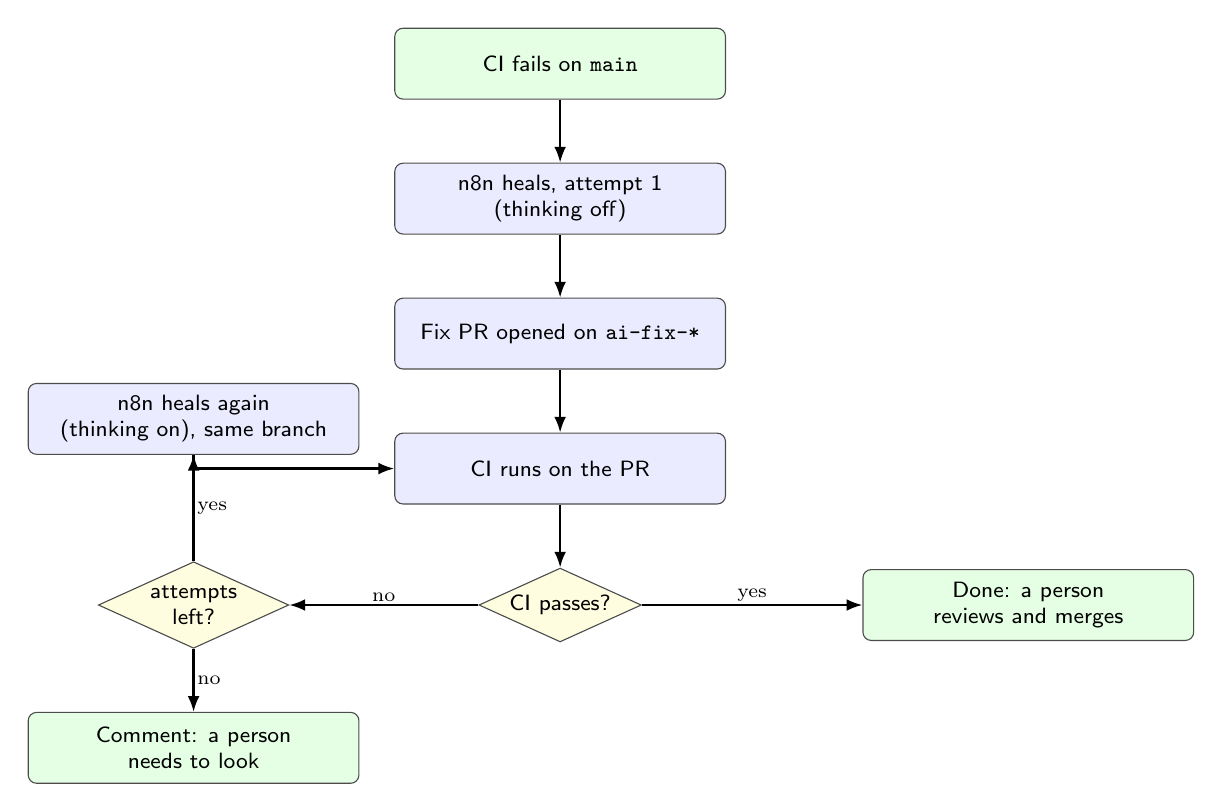
\begin{tikzpicture}[node distance=0.8cm and 1.2cm, every node/.style={font=\sffamily\footnotesize}]
  \node[start] (a) {CI fails on \texttt{main}};
  \node[proc, below=of a] (b) {n8n heals, attempt 1\\(thinking off)};
  \node[proc, below=of b] (c) {Fix PR opened on \texttt{ai-fix-*}};
  \node[proc, below=of c] (d) {CI runs on the PR};
  \node[decision, below=of d] (e) {CI passes?};
  \node[start, right=2.8cm of e] (f) {Done: a person\\reviews and merges};
  \node[decision, left=2.4cm of e] (g) {attempts\\left?};
  \node[proc, above=1.35cm of g] (h) {n8n heals again\\(thinking on), same branch};
  \node[start, below=of g] (i) {Comment: a person\\needs to look};
  \draw[flow] (a) -- (b); \draw[flow] (b) -- (c); \draw[flow] (c) -- (d); \draw[flow] (d) -- (e);
  \draw[flow] (e) -- node[lbl, above]{yes} (f);
  \draw[flow] (e) -- node[lbl, above]{no} (g);
  \draw[flow] (g) -- node[lbl, right]{yes} (h);
  \draw[flow] (h) |- (d);
  \draw[flow] (g) -- node[lbl, right]{no} (i);
\end{tikzpicture}
\caption{The capped retry loop: a failing heal pull request wakes the workflow again, and the attempt number is carried in the commit trailer.}
\label{fig:retry}
\end{figure}


The retry loop is driven by GitHub Actions, not by anything inside n8n. When CI fails on a heal PR, the notify job sends the PR's head branch, its head commit and the trailer number as \texttt{attempt}. In n8n this has four effects. The prompt carries the "Heal attempt N+1" line. Thinking is switched on. The file is fetched at the PR head, so it holds the previous fix. And the new commit goes onto the same branch with the next trailer number. The cap is checked only in the notify job. With \texttt{MAX\_\allowbreak{}ATTEMPTS} set to 3, the first heal and two retries make three attempts, and then the notify job comments that a human is needed.

One detail of the retry shows up at the last step. The new commit is on the PR's own branch, which is also the base that Open Pull Request is given, so GitHub answers 422 "No commits between X and X". Heal Outcome treats this as normal for attempt 2 or later and reports \texttt{retry\_\allowbreak{}pushed}. The need for this was found live: all three retries of one round had pushed correctly and were still marked as failed (source: tools/\allowbreak{}nodes/\allowbreak{}heal\_\allowbreak{}outcome.js, comment; docs/\allowbreak{}results/\allowbreak{}GOLIVE\_\allowbreak{}RESULTS.md, Round 3).

\section{Idempotent re-runs}

The same failed commit can reach the workflow twice, for example when someone re-runs the CI job. The workflow is built so that the second run updates the first one's work instead of breaking. The branch name ends in the first 7 characters of the commit, so the same commit gives the same name when the model repeats its choice. A repeat of the same commit lands on the same branch (a measured case, according to a comment in tools/\allowbreak{}nodes/\allowbreak{}extract\_\allowbreak{}ai\_\allowbreak{}response.js). Create Branch tolerates the 422, Get File SHA reads the file's current blob on that branch, Push Fix File updates it, and if the PR already exists, Heal Outcome reports \texttt{pr\_\allowbreak{}already\_\allowbreak{}open} and leaves it alone.

This holds only when the model proposes the same branch name. Because the name comes from the model, a different name for the same commit would open a second branch and a second PR. We did not test that case.

% GENERATED by build_chapters.py; edit docs/report/chapters, not this file

\chapter{The Model Endpoint}

\section{Role of the service}

The healer needs a language model that n8n and the backend can call over HTTPS. We could not pay for a hosted API, so the model runs on a free Kaggle notebook. A Python script starts a \texttt{llama-\allowbreak{}server} process from the llama.cpp project, loads Qwen3.8-27B into it, and puts a Cloudflare tunnel in front of port 8000. The result is an OpenAI-style chat API (\texttt{/\allowbreak{}v1/\allowbreak{}chat/\allowbreak{}completions}) at a temporary web address.

Everything that runs on Kaggle is one file, \texttt{kaggle/\allowbreak{}endpoint/\allowbreak{}deploy\_\allowbreak{}src.\allowbreak{}py}. A small build script pastes the chosen model entry from \texttt{kaggle/\allowbreak{}endpoint/\allowbreak{}models.\allowbreak{}json} into it and writes the file that is uploaded (\texttt{kaggle/\allowbreak{}tools/\allowbreak{}build\_\allowbreak{}endpoint.\allowbreak{}py}). Boot logs from each session are kept under \texttt{kaggle/\allowbreak{}logs/\allowbreak{}endpoint/\allowbreak{}qwen3-\allowbreak{}8-\allowbreak{}27b-\allowbreak{}live-\allowbreak{}endpoint/\allowbreak{}\textless{}run\textgreater{}/\allowbreak{}}. In this chapter "boot log v16" means the \texttt{boot.\allowbreak{}log} in the run folder whose name ends in \texttt{v16}.

This chapter was checked against the code and the saved logs.

\section{Hardware}

The kernel is private, has the GPU and internet switched on, and sets \texttt{machine\_\allowbreak{}shape} to \texttt{NvidiaTeslaT4} (source: \texttt{kaggle/\allowbreak{}endpoint/\allowbreak{}push/\allowbreak{}kernel-\allowbreak{}metadata.\allowbreak{}json}). That setting matters: with only \texttt{enable\_\allowbreak{}gpu} Kaggle hands out a single P100 instead of two T4 cards, and the notebook's accelerator menu is overwritten by a command-line push (source: \texttt{docs/\allowbreak{}research/\allowbreak{}KAGGLE\_\allowbreak{}ENV\_\allowbreak{}MEASURED.\allowbreak{}md}). The same note measured 4 CPU cores and 31 GB of RAM on the machine.

The boot logs show two Tesla T4 cards with 15360 MiB each, 30720 MiB in total (source: boot log v16). The script adds up the memory that \texttt{nvidia-\allowbreak{}smi} reports. If the sum is below 24000 MiB it prints \texttt{ABORT:\allowbreak{} need 2xT4} and stops before it downloads 17 GB for nothing (source: \texttt{deploy\_\allowbreak{}src.\allowbreak{}py}).

\section{The server binary}

Compiling llama.cpp with CUDA on the four slow cores of a Kaggle machine took about 40 minutes (source: module docstring of \texttt{deploy\_\allowbreak{}src.\allowbreak{}py}). The project therefore builds the server once, in a separate kernel called \texttt{linsxav/\allowbreak{}llama-\allowbreak{}server-\allowbreak{}builder}, and attaches that kernel as a source (\texttt{kernel\_\allowbreak{}sources} in the metadata). At boot the script finds \texttt{llama-\allowbreak{}server-\allowbreak{}cuda.\allowbreak{}zip} under \texttt{/\allowbreak{}kaggle/\allowbreak{}input}, unpacks it into \texttt{/\allowbreak{}kaggle/\allowbreak{}working/\allowbreak{}bin}, sets \texttt{LD\_\allowbreak{}LIBRARY\_\allowbreak{}PATH} and asserts that \texttt{llama-\allowbreak{}server -\allowbreak{}-\allowbreak{}help} runs. Unpacking took 3.5 to 7.0 seconds in the kernel logs we kept (source: \texttt{kernel.\allowbreak{}log} of v11 and v14). If the zip is missing, the script lists the input folder and stops. It has no fallback to compiling.

The build in production is a stock llama.cpp build, which \texttt{docs/\allowbreak{}results/\allowbreak{}GOLIVE\_\allowbreak{}RESULTS.\allowbreak{}md} calls b9690. The quality study in Chapter 9 used a newer fork, b10709, which measured about 4 percent faster on the same settings (source: \texttt{docs/\allowbreak{}results/\allowbreak{}SPEED\_\allowbreak{}QUALITY\_\allowbreak{}EVAL.\allowbreak{}md}).

\section{Model file and quantization}

The model is \texttt{Qwen3.\allowbreak{}8-\allowbreak{}27B-\allowbreak{}UD-\allowbreak{}Q4\_\allowbreak{}K\_\allowbreak{}XL.\allowbreak{}gguf} from the Hugging Face repository \texttt{unsloth/\allowbreak{}Qwen3.\allowbreak{}8-\allowbreak{}27B-\allowbreak{}GGUF}, 17.6 GB (source: \texttt{kaggle/\allowbreak{}endpoint/\allowbreak{}models.\allowbreak{}json}). GGUF is the single-file format llama.cpp reads: it holds the weights, the tokenizer and the chat template together. A name like Q4\_\allowbreak{}K\_\allowbreak{}XL says how the weights were compressed: roughly 4-bit blocks of the "K" kind, with the "XL" mix keeping some tensors at higher precision, and the "UD" prefix marks Unsloth's dynamic variant (this reading of the name is general knowledge about the format, not something the project measured). For scale, 17.6 GB over about 27 billion weights is around 5 bits per weight on average (our arithmetic from those two figures).

\texttt{fetch()} in the script lists the \texttt{.\allowbreak{}gguf} files in the repository, skips anything with \texttt{mmproj} in its name, and downloads the first file that matches the registry pattern. If that fails it tries \texttt{UD-\allowbreak{}Q4\_\allowbreak{}K\_\allowbreak{}M} and then \texttt{UD-\allowbreak{}Q6\_\allowbreak{}K} from the same repository. Downloads took 65 s (v8), 363 s (v9), 92 s (v10), 84 s (v11), 91 s (v12), 89 s and 76 s (the two attempts logged under v14), and 82 s (v16) (source: boot logs of those runs). Only v9 was slow, and the logs do not say why.

The default stayed because of the four-model bake-off: it tied the others on first-try heals (14 of 24), healed 21 of 24 with thinking on against 15 to 17 for the others, and was the fastest (source: \texttt{docs/\allowbreak{}results/\allowbreak{}MODEL\_\allowbreak{}BAKEOFF.\allowbreak{}md}; Chapter 9).

\section{Server flags}

\texttt{launch()} kills any old server, waits 4 seconds and starts a new one in the background. The flags are these (source: \texttt{deploy\_\allowbreak{}src.\allowbreak{}py}, \texttt{launch()}).

\begingroup\small
\begin{longtable}{>{\raggedright\arraybackslash}p{0.439\dimexpr\linewidth-4\tabcolsep\relax}>{\raggedright\arraybackslash}p{0.561\dimexpr\linewidth-4\tabcolsep\relax}}
\toprule
\rowcolor{gray!14}\textbf{Flag} & \textbf{Effect} \\
\midrule
\endhead
\bottomrule
\endfoot
\endlastfoot
\texttt{-\allowbreak{}m \textless{}file\textgreater{}} & The downloaded GGUF file. \\
\texttt{-\allowbreak{}-\allowbreak{}n-\allowbreak{}gpu-\allowbreak{}layers 999} & Put every layer on the GPUs. \\
\texttt{-\allowbreak{}-\allowbreak{}ctx-\allowbreak{}size \textless{}n\textgreater{}} & Context length, taken from the ladder below. \\
\texttt{-\allowbreak{}-\allowbreak{}flash-\allowbreak{}attn on} & Flash attention. It was already on before the speed work, and tensor split needs it (source: \texttt{docs/\allowbreak{}results/\allowbreak{}SPEED\_\allowbreak{}LEVERS\_\allowbreak{}EVAL.\allowbreak{}md}). \\
\texttt{-\allowbreak{}sm tensor} & Split every tensor across both cards so both read weights at the same time. The default splits by layer, and the cards then work one after the other. \\
\texttt{-\allowbreak{}-\allowbreak{}cache-\allowbreak{}type-\allowbreak{}k f16 -\allowbreak{}-\allowbreak{}cache-\allowbreak{}type-\allowbreak{}v f16} & Unquantized attention cache. Tensor mode forbids a quantized cache, so these flags and \texttt{-\allowbreak{}sm tensor} change together (source: \texttt{docs/\allowbreak{}results/\allowbreak{}SPEED\_\allowbreak{}LEVERS\_\allowbreak{}EVAL.\allowbreak{}md}). \\
\texttt{-\allowbreak{}-\allowbreak{}spec-\allowbreak{}type draft-\allowbreak{}mtp -\allowbreak{}-\allowbreak{}spec-\allowbreak{}draft-\allowbreak{}n-\allowbreak{}max 2} & Speculative decoding with the model's own multi-token-prediction head: it drafts up to 2 tokens and the full model checks them in one pass. \\
\texttt{-\allowbreak{}-\allowbreak{}parallel 1} and \texttt{-\allowbreak{}np 1} & One request slot. These are the same option written twice. Heal requests arrive one at a time. \\
\texttt{-\allowbreak{}b 2048 -\allowbreak{}ub 512} & Batch and micro-batch size for reading the prompt. \\
\texttt{-\allowbreak{}t 4 -\allowbreak{}tb 4} & Four CPU threads for generation and four for prompt batches. \\
\texttt{-\allowbreak{}-\allowbreak{}reasoning-\allowbreak{}budget 1024} & Cap on thinking tokens when thinking is on. The code has no comment on it. \\
\texttt{-\allowbreak{}-\allowbreak{}host 0.\allowbreak{}0.\allowbreak{}0.\allowbreak{}0 -\allowbreak{}-\allowbreak{}port 8000} & Listen on port 8000 on all interfaces. \\
\texttt{-\allowbreak{}-\allowbreak{}jinja} & Use the chat template stored in the model file. \\
\texttt{-\allowbreak{}-\allowbreak{}api-\allowbreak{}key selfheal-\allowbreak{}e2e-\allowbreak{}key} & Require \texttt{Authorization:\allowbreak{} Bearer \textless{}key\textgreater{}}. \\
\texttt{-\allowbreak{}-\allowbreak{}chat-\allowbreak{}template-\allowbreak{}kwargs '\{"enable\_\allowbreak{}thinking":\allowbreak{}false\}'} & Default thinking to off. It is added only if the binary's help text lists this option. \\
\bottomrule
\caption{Server flags}\label{tab:07-1}\\
\end{longtable}
\endgroup

The speed work behind \texttt{-\allowbreak{}sm tensor} and MTP is in the last section of this chapter and in Chapter 9. Before it, the production flags used a quantized \texttt{q8\_\allowbreak{}0} cache and layer split (source: \texttt{docs/\allowbreak{}results/\allowbreak{}SPEED\_\allowbreak{}LEVERS\_\allowbreak{}EVAL.\allowbreak{}md}, "What shipping looks like").

\section{Context ladder}

\begin{figure}[!htbp]
\centering
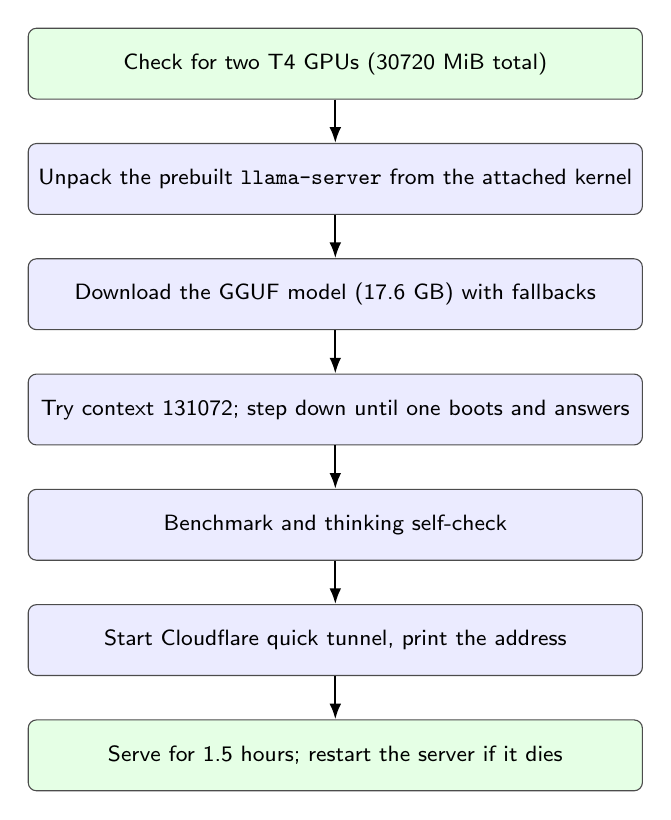
\begin{tikzpicture}[node distance=0.55cm, every node/.style={font=\sffamily\footnotesize}]
  \node[start, minimum width=7.8cm] (a) {Check for two T4 GPUs (30720 MiB total)};
  \node[proc, minimum width=7.8cm, below=of a] (b) {Unpack the prebuilt \texttt{llama-server} from the attached kernel};
  \node[proc, minimum width=7.8cm, below=of b] (c) {Download the GGUF model (17.6 GB) with fallbacks};
  \node[proc, minimum width=7.8cm, below=of c] (d) {Try context 131072; step down until one boots and answers};
  \node[proc, minimum width=7.8cm, below=of d] (e) {Benchmark and thinking self-check};
  \node[proc, minimum width=7.8cm, below=of e] (f) {Start Cloudflare quick tunnel, print the address};
  \node[start, minimum width=7.8cm, below=of f] (g) {Serve for 1.5 hours; restart the server if it dies};
  \foreach \x/\y in {a/b,b/c,c/d,d/e,e/f,f/g} \draw[flow] (\x) -- (\y);
\end{tikzpicture}
\caption{Boot sequence of the endpoint kernel on Kaggle.}
\label{fig:boot}
\end{figure}


The script tries context sizes of 131072, 98304, 65536, 32768, 16384 and 8192 tokens, largest first. Each try gets 300 seconds for \texttt{/\allowbreak{}health} to answer 200, and the wait ends early if the server process has died. A rung that boots must also answer three benchmark requests. The first rung that does is kept, and the script asserts if none does (source: \texttt{deploy\_\allowbreak{}src.\allowbreak{}py}, \texttt{LADDER}).

The ladder used to start higher. In the first live round, sizes of 262144 and 196608 each hung for the full 15-minute health timeout, about 30 minutes of GPU time, before 131072 booted in under a minute. With tensor split, llama.cpp cannot fit the context to memory by itself, so a rung that is too large does not fail quickly (source: \texttt{docs/\allowbreak{}results/\allowbreak{}GOLIVE\_\allowbreak{}RESULTS.\allowbreak{}md}, "Three defects found only by going live"; the server log of v11 has the warning \texttt{llama\_\allowbreak{}params\_\allowbreak{}fit is not implemented for SPLIT\_\allowbreak{}MODE\_\allowbreak{}TENSOR}). The model was trained for 262144 tokens, and the log of v11 says the 131072 setting leaves part of that unused.

Every boot log we kept shows the first rung, 131072, booting (source: boot logs v8 to v16). Memory in use afterwards was 26566 MiB of 30720 MiB in v8 to v12 and 26662 MiB in v15 and v16 (source: the same logs). The research notes explain why this fits: only 16 of the model's 64 layers keep a cache that grows with the context (source: \texttt{docs/\allowbreak{}research/\allowbreak{}QWEN38\_\allowbreak{}HARDWARE\_\allowbreak{}FACTS.\allowbreak{}md}, a secondary source, not measured by us).

\section{Thinking default}

Qwen3.8's chat template makes the model think before it answers unless a request says otherwise. The v11 server log reads \texttt{chat template, thinking = 1} (source: \texttt{server.\allowbreak{}log} of v11). The n8n workflow always sends \texttt{enable\_\allowbreak{}thinking} with each request: false on the first heal and true on a retry (source: \texttt{tools/\allowbreak{}nodes/\allowbreak{}build\_\allowbreak{}ai\_\allowbreak{}prompt.\allowbreak{}js}, line 155). The backend sends it only to turn thinking on, so before the change every backend call would have thought first. The classifier asks for at most 512 tokens, and thinking tokens count against that limit, so a long thought could leave no room for the JSON answer (source: \texttt{docs/\allowbreak{}results/\allowbreak{}BACKEND\_\allowbreak{}ON\_\allowbreak{}KAGGLE.\allowbreak{}md}).

The kernel therefore starts the server with thinking off, and a request that sets \texttt{enable\_\allowbreak{}thinking:\allowbreak{} true} still turns it on. Thinking is expensive: in the shipped-quality study the median call took 36.8 s with it and 9.1 s without (source: \texttt{docs/\allowbreak{}results/\allowbreak{}SHIPPED\_\allowbreak{}QUALITY\_\allowbreak{}EVAL.\allowbreak{}md}). The policy that follows is thinking off for the first attempt and on for a retry, which the n8n chapter describes.

\section{Boot-time self-check}

After a rung boots, the script does not trust its own flags. \texttt{bench()} sends three requests of up to 256 tokens at temperature 0.7 and reads the server's own \texttt{timings} field, not the log text. From that it works out three facts:

\begin{itemize}[leftmargin=*, itemsep=2pt]
\item \textbf{Tensor split engaged.} True when the two cards report memory use within 64 MiB of each other. Layer split leaves them uneven, tensor split makes them equal.
\item \textbf{MTP engaged.} True when at least one request reported draft tokens.
\item \textbf{Accept rate.} Accepted draft tokens divided by drafted tokens.
\end{itemize}

If either lever is missing the script prints a warning that the endpoint will be slower than measured, and serves anyway. This design came from two earlier mistakes in which a log-wording check reported a working lever as missing (source: \texttt{docs/\allowbreak{}results/\allowbreak{}SPEED\_\allowbreak{}LEVERS\_\allowbreak{}EVAL.\allowbreak{}md} and \texttt{docs/\allowbreak{}results/\allowbreak{}SPEED\_\allowbreak{}QUALITY\_\allowbreak{}EVAL.\allowbreak{}md}).

\texttt{thinking\_\allowbreak{}check()} then asks "What is 17 * 23?" twice, once plain and once with thinking requested. A reply counts as thinking if it has \texttt{reasoning\_\allowbreak{}content} or a \texttt{\textless{}think\textgreater{}} block. The expected result is false then true. Boot logs v14, v15 and v16 all show \texttt{thinking by default :\allowbreak{} False} and \texttt{thinking when asked :\allowbreak{} True} with the answer 391 both times (source: \texttt{stream.\allowbreak{}log} of v14 and v15, \texttt{boot.\allowbreak{}log} of v16). The older runs v8 to v12 predate this check.

In the saved files v12 has no thinking-check lines and v14, v15 and v16 do.

The boot benchmark of each session that reached the end was this (source: the \texttt{SELECTED} lines of the boot logs).

\begingroup\small
\begin{longtable}{>{\raggedright\arraybackslash}p{0.198\dimexpr\linewidth-10\tabcolsep\relax}>{\raggedright\arraybackslash}p{0.272\dimexpr\linewidth-10\tabcolsep\relax}>{\raggedright\arraybackslash}p{0.198\dimexpr\linewidth-10\tabcolsep\relax}>{\raggedright\arraybackslash}p{0.148\dimexpr\linewidth-10\tabcolsep\relax}>{\raggedright\arraybackslash}p{0.185\dimexpr\linewidth-10\tabcolsep\relax}}
\toprule
\rowcolor{gray!14}\textbf{Session} & \textbf{Date} & \textbf{Average tok/\allowbreak{}s} & \textbf{Best tok/\allowbreak{}s} & \textbf{MTP accept rate} \\
\midrule
\endhead
\bottomrule
\endfoot
\endlastfoot
v8 & 2026-09-23 & 26.4 & 26.6 & 0.671 \\
v9 & 2026-09-23 & 26.6 & 27.5 & 0.633 \\
v10 & 2026-09-28 & 24.0 & 25.0 & 0.64 \\
v11 & 2026-09-28 & 23.9 & 24.4 & 0.613 \\
v12 & 2026-10-30 & 23.8 & 24.4 & 0.64 \\
v15 & 2026-11-15 & 26.8 & 27.4 & 0.664 \\
v16 & 2026-11-15 & 22.4 & 23.7 & 0.719 \\
\bottomrule
\caption{Boot-time self-check}\label{tab:07-2}\\
\end{longtable}
\endgroup

All seven had the tensor split engaged, with equal memory on both cards (source: the same logs). Version 14 and version 15 look like two sessions in the log folders, but the v14 kernel log shows a \texttt{TypeError} in \texttt{launch()} at the first rung, so v14 never served. Its \texttt{stream.\allowbreak{}log} continues with the output of v15, which was pushed about 3 minutes later (source: \texttt{kernel.\allowbreak{}log} of v14 and \texttt{history.\allowbreak{}jsonl}), and the two runs report the same tunnel address. This chapter counts them as one session.

The accept rates here are far below the 0.95 to 0.96 measured on real code fixes (source: \texttt{docs/\allowbreak{}results/\allowbreak{}SPEED\_\allowbreak{}LEVERS\_\allowbreak{}EVAL.\allowbreak{}md}). The boot benchmark asks for a general explanation at temperature 0.7, and that text is harder to guess than a code edit. Speed also varied between sessions from 22.4 to 26.8 tok/\allowbreak{}s with the same flags. The documents give no reason.

\section{Tunnel and changing address}

When the benchmark is done, the script downloads \texttt{cloudflared} and starts \texttt{cloudflared tunnel -\allowbreak{}-\allowbreak{}url http:\allowbreak{}/\allowbreak{}/\allowbreak{}localhost:\allowbreak{}8000}. It reads \texttt{tunnel.\allowbreak{}log} every 4 seconds, up to 45 times, until a \texttt{https:\allowbreak{}/\allowbreak{}/\allowbreak{}\textless{}words\textgreater{}.\allowbreak{}trycloudflare.\allowbreak{}com} address appears. This is a quick tunnel: it needs no Cloudflare account, and every start gets a new random name. The saved boot logs show seven different addresses for the seven sessions, for example \texttt{pilot-\allowbreak{}fixed-\allowbreak{}cooler-\allowbreak{}hello} in v8 and \texttt{hats-\allowbreak{}conducted-\allowbreak{}committees-\allowbreak{}hollywood} in v16.

A quick tunnel also cuts a request that stays silent for 120 seconds. An unstreamed request through it failed with HTTP 524 at 125.9 s, while the same request streamed succeeded after 166.5 s with 3600 tokens (source: \texttt{eval/\allowbreak{}runs/\allowbreak{}golive5/\allowbreak{}golive5\_\allowbreak{}stream\_\allowbreak{}proof.\allowbreak{}json}). Both the n8n workflow and the backend therefore ask for streamed replies. Only port 8000 is exposed, and the server still checks the API key. The key is a constant in the repository, so anyone who can read the repository can read it.

\section{Session window}

After the tunnel step the script writes \texttt{endpoint.\allowbreak{}json} and sets a deadline of \texttt{HOURS = 1.\allowbreak{}5} from that moment. The comment gives the reason: the Kaggle command line cannot reliably cancel a running kernel, so the script ends itself. Once a minute the loop checks for a \texttt{llama-\allowbreak{}server} process and restarts it at the chosen context if none is found, and the tunnel stays up, so the address does not change. Every ten minutes it prints the full "ENDPOINT LIVE" block again and on other minutes a one-line status.

The log of v11 matches this. It reached the URL line at 223 s (3.5 s unpacking, 84 s download, about 90 s to boot, 34 s benchmark, 8 s tunnel) and its script output ends at about 94 minutes, which is 223 s plus 90 minutes (source: \texttt{kernel.\allowbreak{}log} of v11). The first live round used a window of 1.0 hours and the third round moved it to 1.5 (source: \texttt{docs/\allowbreak{}results/\allowbreak{}GOLIVE\_\allowbreak{}RESULTS.\allowbreak{}md}). The launcher script quotes about 4 minutes from push to a usable address (source: \texttt{launcher/\allowbreak{}README.\allowbreak{}md}).

\section{How the address reaches n8n and the backend}

\texttt{kaggle/\allowbreak{}tools/\allowbreak{}watch\_\allowbreak{}deploy.\allowbreak{}py} follows the kernel log, and when it sees the \texttt{URL :\allowbreak{}} line it writes the address to \texttt{\%LOCALAPPDATA\%\textbackslash{}selfheal-\allowbreak{}n8n\textbackslash{}qwen\_\allowbreak{}url.\allowbreak{}txt}, outside the repository. Two scripts read that file.

\begin{itemize}[leftmargin=*, itemsep=2pt]
\item \textbf{n8n.} \texttt{tools/\allowbreak{}golive/\allowbreak{}set\_\allowbreak{}cloud\_\allowbreak{}qwen\_\allowbreak{}url.\allowbreak{}py} posts the address to the cloud workflow's \texttt{set-\allowbreak{}qwen-\allowbreak{}url} webhook, with a secret header. The node \texttt{Store Model URL} accepts only addresses that match \texttt{https:\allowbreak{}/\allowbreak{}/\allowbreak{}*.\allowbreak{}trycloudflare.\allowbreak{}com} and saves the address in the workflow's static data. The node \texttt{Get Model URL} reads it before each model call and falls back to the n8n variable \texttt{QWEN\_\allowbreak{}BASE\_\allowbreak{}URL} (source: \texttt{tools/\allowbreak{}nodes/\allowbreak{}store\_\allowbreak{}model\_\allowbreak{}url.\allowbreak{}js}, \texttt{tools/\allowbreak{}nodes/\allowbreak{}get\_\allowbreak{}model\_\allowbreak{}url.\allowbreak{}js}). A webhook is used because the n8n API is switched off on cloud trials.
\item \textbf{Backend.} \texttt{kaggle/\allowbreak{}tools/\allowbreak{}backend\_\allowbreak{}env.\allowbreak{}py} rewrites the \texttt{CLASSIFIER\_\allowbreak{}} and \texttt{FIXER\_\allowbreak{}} lines for provider, base URL, key and model name in \texttt{ci-\allowbreak{}heal-\allowbreak{}backend/\allowbreak{}.\allowbreak{}env}, and with \texttt{-\allowbreak{}-\allowbreak{}check} calls \texttt{GET /\allowbreak{}v1/\allowbreak{}models} through the tunnel (source: \texttt{kaggle/\allowbreak{}tools/\allowbreak{}backend\_\allowbreak{}env.\allowbreak{}py}). It has to run again after every boot.
\end{itemize}

The one-click start file \texttt{launcher/\allowbreak{}start/\allowbreak{}1\_\allowbreak{}start\_\allowbreak{}model\_\allowbreak{}on\_\allowbreak{}kaggle.\allowbreak{}bat} runs the status check, build, push, watch and webhook steps in order. A failed webhook step only prints a message, so the model can be running while n8n still holds the old address. In that case the Qwen call fails and the workflow goes to its OpenAI fallback and then to a failure comment.

\section{Quota and stopping}

A Kaggle quota dialog read on 2026-09-07 showed 30 hours of GPU per week (source: \texttt{docs/\allowbreak{}research/\allowbreak{}KAGGLE\_\allowbreak{}ENV\_\allowbreak{}MEASURED.\allowbreak{}md}). The figure is from one dialog on one day, and Kaggle may change it. At 1.5 hours per window and ignoring boot time, 30 hours is at most 20 windows a week (our arithmetic).

A push does not replace a running kernel. Kaggle starts a second session, which would use quota twice, so \texttt{push.\allowbreak{}py} refuses to push while any of the four project kernels is \texttt{RUNNING} or \texttt{QUEUED} unless \texttt{-\allowbreak{}-\allowbreak{}force} is given. The Kaggle README adds that GPU kernels can wait in the queue for hours (source: \texttt{kaggle/\allowbreak{}README.\allowbreak{}md}).

The command line cannot stop a session. The helper \texttt{launcher/\allowbreak{}end/\allowbreak{}stop\_\allowbreak{}model\_\allowbreak{}on\_\allowbreak{}kaggle.\allowbreak{}bat} opens the kernel page and prints the steps: View Active Events, the session menu, Stop Session. \texttt{history.\allowbreak{}jsonl} records two manual stops through the website, for v12 and v15, and v12 ended with status \texttt{CANCEL\_\allowbreak{}ACKNOWLEDGED} (source: \texttt{history.\allowbreak{}jsonl}). A session nobody stops runs out its 1.5 hours and uses quota the whole time. This is a real limit of the setup, because it depends on a person remembering to stop it, and the endpoint is a development service, not a durable host (source: \texttt{kaggle/\allowbreak{}README.\allowbreak{}md}).

\section{Measured speed}

Speed was measured in four settings, and the figures do not belong in one column, so the table names the setting of each.

\begingroup\small
\begin{longtable}{>{\raggedright\arraybackslash}p{0.348\dimexpr\linewidth-6\tabcolsep\relax}>{\raggedright\arraybackslash}p{0.167\dimexpr\linewidth-6\tabcolsep\relax}>{\raggedright\arraybackslash}p{0.486\dimexpr\linewidth-6\tabcolsep\relax}}
\toprule
\rowcolor{gray!14}\textbf{Setting} & \textbf{Median tok/\allowbreak{}s} & \textbf{Source} \\
\midrule
\endhead
\bottomrule
\endfoot
\endlastfoot
First 9-config sweep, layer split, no MTP & 8.8 for the chosen file & \texttt{docs/\allowbreak{}old/\allowbreak{}QWEN38\_\allowbreak{}SWEEP\_\allowbreak{}RESULTS.\allowbreak{}md} \\
First live round trip, old flags (\texttt{q8\_\allowbreak{}0} cache, layer split) & 12.11 mean & \texttt{docs/\allowbreak{}old/\allowbreak{}SELFHEAL\_\allowbreak{}E2E\_\allowbreak{}RESULTS.\allowbreak{}md} \\
Speed rig A, same old flags, ctx 8192 & 12.35 & \texttt{docs/\allowbreak{}results/\allowbreak{}SPEED\_\allowbreak{}LEVERS\_\allowbreak{}EVAL.\allowbreak{}md} \\
Rig B, \texttt{-\allowbreak{}sm tensor} with f16 cache & 15.49 (+25\%) & \texttt{docs/\allowbreak{}results/\allowbreak{}SPEED\_\allowbreak{}LEVERS\_\allowbreak{}EVAL.\allowbreak{}md} \\
Rig C, MTP only & 19.99 (+62\%) & \texttt{docs/\allowbreak{}results/\allowbreak{}SPEED\_\allowbreak{}LEVERS\_\allowbreak{}EVAL.\allowbreak{}md} \\
Rig D, both levers & 26.83 (+117\%) & \texttt{docs/\allowbreak{}results/\allowbreak{}SPEED\_\allowbreak{}LEVERS\_\allowbreak{}EVAL.\allowbreak{}md} \\
Fork build b10709, both levers & 28.02 & \texttt{docs/\allowbreak{}results/\allowbreak{}SPEED\_\allowbreak{}QUALITY\_\allowbreak{}EVAL.\allowbreak{}md} \\
Boot benchmark, seven sessions, ctx 131072 & 22.4 to 26.8 average & boot logs v8 to v16 \\
Live decode, round 1 & 23.10 & \texttt{docs/\allowbreak{}results/\allowbreak{}GOLIVE\_\allowbreak{}RESULTS.\allowbreak{}md} \\
Live decode, round 2 & 27.73 & \texttt{docs/\allowbreak{}results/\allowbreak{}GOLIVE\_\allowbreak{}RESULTS.\allowbreak{}md} \\
Bake-off baseline, ctx 131072 & 23.4 & \texttt{docs/\allowbreak{}results/\allowbreak{}MODEL\_\allowbreak{}BAKEOFF.\allowbreak{}md} \\
\bottomrule
\caption{Measured speed}\label{tab:07-3}\\
\end{longtable}
\endgroup

We recomputed rigs A to D from \texttt{eval/\allowbreak{}runs/\allowbreak{}kout\_\allowbreak{}speed/\allowbreak{}results.\allowbreak{}json}: 60 calls, no errors, and the same medians. In rig D the MTP head accepted drafts at a median rate of 0.96, and the per-card memory was 9051 MiB on each card, against uneven pairs such as 7761 and 9371 MiB in rig A (source: the same file). The tensor-split gain is smaller than the +47 to +68 percent reported for Ampere machines. The study traces this to PCIe: the two T4 cards have no NVLink, and it estimates the cost of combining results at about 24 ms per token (source: \texttt{docs/\allowbreak{}results/\allowbreak{}SPEED\_\allowbreak{}LEVERS\_\allowbreak{}EVAL.\allowbreak{}md}).

The live figures are lower than the rig because the inputs differ. Round 1 had an MTP accept rate of about 0.89 against 0.965 in the rig, since a search-and-replace answer is less predictable than a whole file that mostly copies the input (source: \texttt{docs/\allowbreak{}results/\allowbreak{}GOLIVE\_\allowbreak{}RESULTS.\allowbreak{}md}). The same document ran with a context of 131072 against 8192 in the rig. Round 2 decoded faster at the same settings, and the document says the reason is not proven.

Prompt reading ran at 274 to 323 tok/\allowbreak{}s in round 1, which is about 2.2 s for a prompt of roughly 700 tokens. A model call through the tunnel carried 5 to 6 s of fixed overhead on top of generation (source: \texttt{docs/\allowbreak{}results/\allowbreak{}GOLIVE\_\allowbreak{}RESULTS.\allowbreak{}md}). The study that set \texttt{-\allowbreak{}-\allowbreak{}spec-\allowbreak{}draft-\allowbreak{}n-\allowbreak{}max} named values 3 and 4 as the next thing to test, and we found no result for them in the documents, so 2 is the value in use but not a tuned one.

% GENERATED by build_chapters.py; edit docs/report/chapters, not this file

\chapter{The ci-heal-backend Service}

\section{Purpose and difference from the n8n healer}

\texttt{ci-\allowbreak{}heal-\allowbreak{}backend} is a FastAPI service that acts as the second healer in this project. It watches for failed GitHub Actions runs, asks a language model what kind of failure it was, and then does one of three things: ask GitHub to re-run the failed jobs, open a pull request with a small fix, or open an issue for a person to read. It starts in a safe mode. \texttt{DRY\_\allowbreak{}RUN} is true by default, so nothing is written to GitHub until the operator sets \texttt{DRY\_\allowbreak{}RUN=false} (source: app/\allowbreak{}config.py).

The first healer is the n8n workflow described in an earlier chapter. It is a chain of workflow nodes that prompts the model and acts on the answer. The backend does the same job as ordinary code with a database behind it. Three differences matter in practice.

\begin{itemize}[leftmargin=*, itemsep=2pt]
\item The decision is made by a pure function, \texttt{decide} in \texttt{app/\allowbreak{}core/\allowbreak{}decision\_\allowbreak{}engine.\allowbreak{}py}, with named thresholds. The model only supplies a category and a confidence. It never chooses the action.
\item Every failure, classification, fix candidate and decision is stored in a database, so attempt budgets, outcomes and calibration statistics can be read back later.
\item A fix is generated several times and the candidates are compared with each other. The pull request is only opened when they agree closely enough.
\end{itemize}

The log trimming rules are a direct port of the \texttt{trimCiLog} function from the n8n "Build AI Prompt" node, so both healers show the model the same kind of log excerpt (source: app/\allowbreak{}core/\allowbreak{}log\_\allowbreak{}trim.py). The two model roles, classifier and fixer, each have their own URL, key and model name, and both can point at the self-hosted Qwen3.8-27B endpoint (source: app/\allowbreak{}config.py).

\section{Request flow}

\begin{figure}[!htbp]
\centering
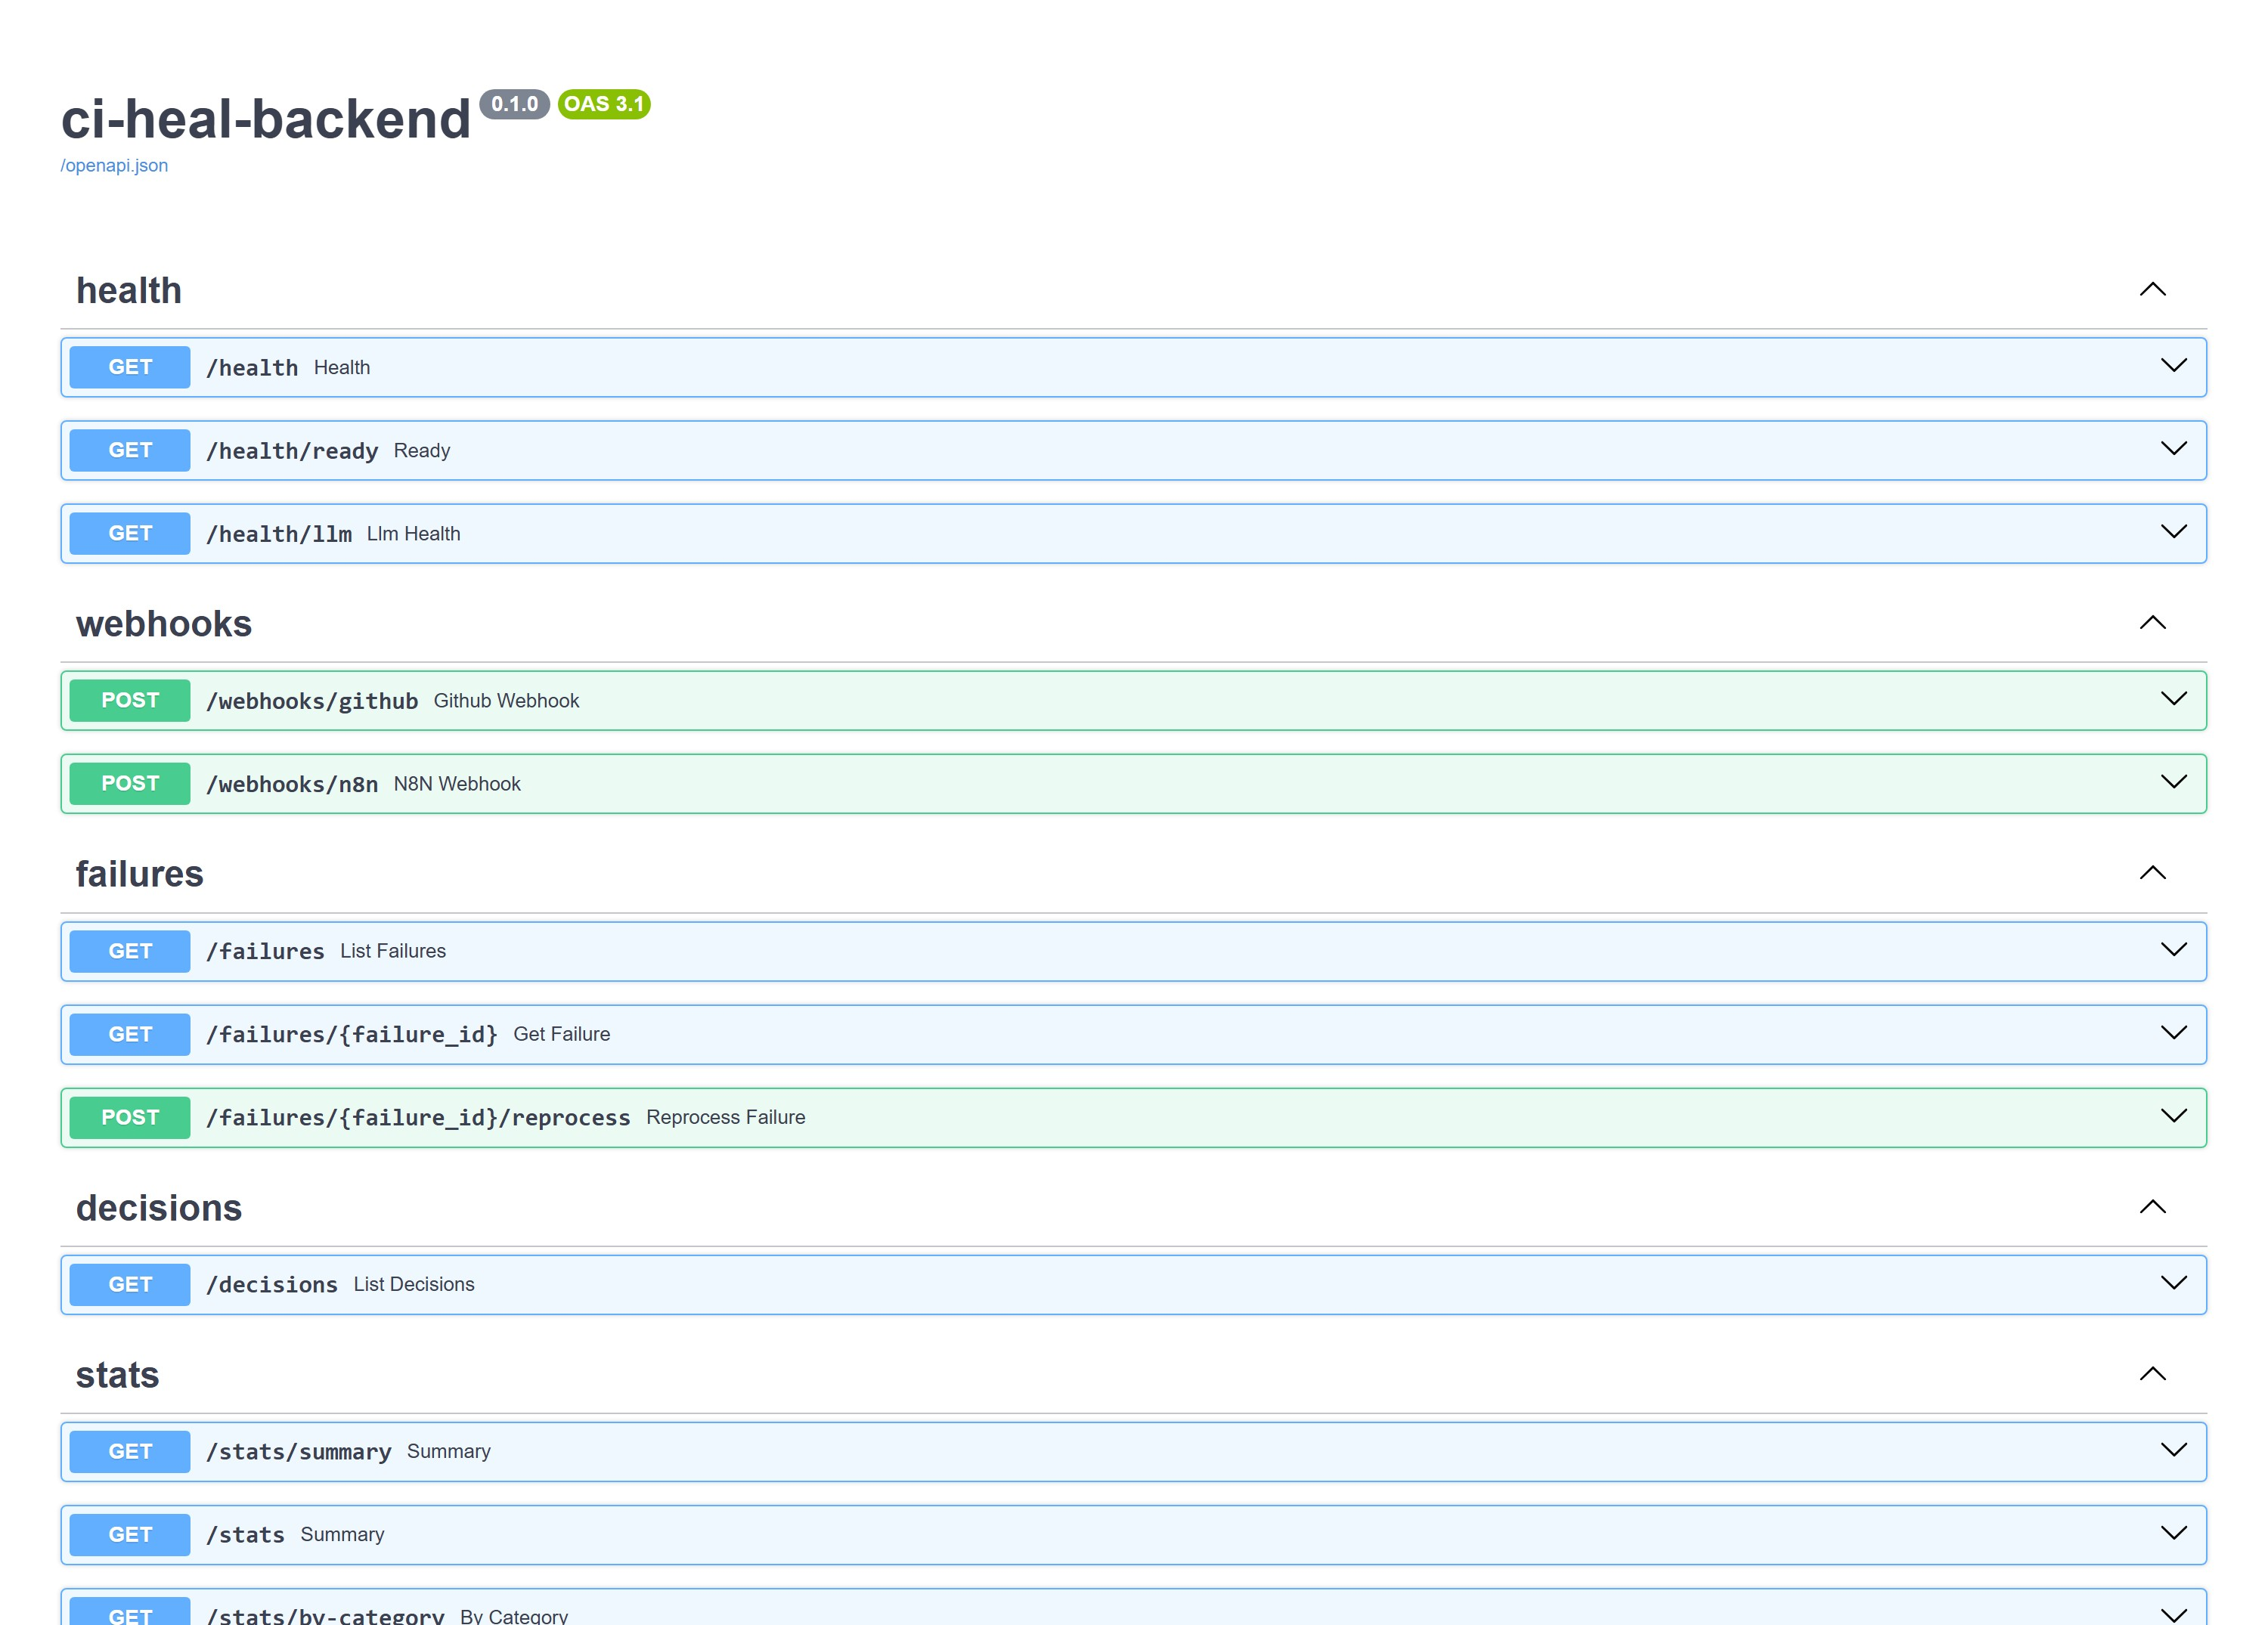
\includegraphics[width=0.88\linewidth]{figures/shots/hq_swagger.jpg}
\caption{The interactive API page of \texttt{ci-heal-backend} (\texttt{/docs}): the health, webhook, failure, decision and statistics endpoints.}
\label{fig:shot-swagger}
\end{figure}


A failure travels through the service in the order below. The numbers refer to the code in \texttt{app/\allowbreak{}api/\allowbreak{}webhooks.\allowbreak{}py} and \texttt{app/\allowbreak{}services/\allowbreak{}orchestrator.\allowbreak{}py}.

\begin{enumerate}[leftmargin=*, itemsep=2pt]
\item \textbf{Webhook.} GitHub posts a \texttt{workflow\_\allowbreak{}run} event to \texttt{POST /\allowbreak{}webhooks/\allowbreak{}github}. n8n can instead post a small JSON body (run id, repo, branch, commit) to \texttt{POST /\allowbreak{}webhooks/\allowbreak{}n8n}, and the backend then loads the real run from the GitHub API. Both routes reduce the delivery to one internal \texttt{IncomingRun} object.
\item \textbf{Authentication.} The GitHub route checks the \texttt{X-\allowbreak{}Hub-\allowbreak{}Signature-\allowbreak{}256} HMAC over the raw body. The n8n route compares the \texttt{X-\allowbreak{}N8N-\allowbreak{}Token} header with \texttt{N8N\_\allowbreak{}SHARED\_\allowbreak{}TOKEN}. A wrong value is a 401. A \texttt{ping} event returns 200.
\item \textbf{Intake rules.} Only a completed run with conclusion \texttt{failure} or \texttt{success} is acted on, and everything else gets 202 with status \texttt{ignored}. The repository must be in \texttt{ALLOWED\_\allowbreak{}REPOS}, and an empty list allows nothing, otherwise the answer is 403. A run on a branch that starts with \texttt{ai-\allowbreak{}fix-\allowbreak{}} is never treated as new work. It is only used to verify an earlier fix. A run whose actor is the token owner (\texttt{GITHUB\_\allowbreak{}BOT\_\allowbreak{}LOGIN}) is ignored, so the bot cannot trigger itself. The body is limited to \texttt{WEBHOOK\_\allowbreak{}MAX\_\allowbreak{}BYTES}, 1,000,000 by default (source: app/\allowbreak{}api/\allowbreak{}webhooks.py, app/\allowbreak{}config.py).
\item \textbf{Claim.} The failure row is unique on repo, run id and run attempt, so a repeated delivery returns \texttt{duplicate}. The row is saved as \texttt{queued}, the request returns 202, and a background task takes over. The worker moves the row to \texttt{processing} with one UPDATE that only matches a row still in \texttt{queued}, so two workers cannot take the same failure (source: app/\allowbreak{}db/\allowbreak{}repositories.py).
\item \textbf{Fetch evidence.} The worker downloads the run log zip, compares the commit with its parent to get a diff, and loads up to eight files that the diff touches. The log token is not forwarded to the redirect host that serves the zip (source: app/\allowbreak{}services/\allowbreak{}github\_\allowbreak{}client.py, app/\allowbreak{}services/\allowbreak{}orchestrator.py).
\item \textbf{Redact and trim.} Secrets in the log, diff and files are replaced with \texttt{[REDACTED:\allowbreak{}\textless{}KIND\textgreater{}]} placeholders first. Only then is the log cut to the failure region: from the last \texttt{\#\#[endgroup]} before the first \texttt{\#\#[error]} line, at most 40 lines and 3000 characters. Redacting first matters because a secret outside the kept region would otherwise escape the count (source: app/\allowbreak{}services/\allowbreak{}secret\_\allowbreak{}redactor.py, app/\allowbreak{}core/\allowbreak{}log\_\allowbreak{}trim.py).
\item \textbf{Classify.} The classifier role returns one of four categories with a confidence. The result is stored as a classification row.
\item \textbf{Decision stage 1.} The engine sees the category, the confidence, the retry count and the attempt count. It answers retry, escalate, or candidate fix.
\item \textbf{Fixer.} For a candidate fix, the fixer role is asked for \texttt{FIX\_\allowbreak{}CANDIDATES} patches (3 by default), one after another, at temperature 0.7. Each reply must be a JSON object with a file path and SEARCH/\allowbreak{}REPLACE edits. Each patch is applied to the original file text in memory and checked by the guards described below. A call that fails or a patch that does not apply becomes an invalid candidate and does not stop the others (source: app/\allowbreak{}services/\allowbreak{}fix\_\allowbreak{}generator.py).
\item \textbf{Agreement and stage 2.} Candidates are scored against each other. The engine runs again with the agreement score and answers fix or escalate.
\item \textbf{Act.} A fix opens a pull request. An escalation opens an issue. A retry asks GitHub to re-run the failed jobs. In dry-run each of these is only logged and a placeholder URL is stored.
\item \textbf{Verify later.} When a later \texttt{workflow\_\allowbreak{}run} arrives, the backend closes the open decision. A re-run of a retried run closes the retry as \texttt{retry\_\allowbreak{}success} or \texttt{retry\_\allowbreak{}failure}. A run on the \texttt{ai-\allowbreak{}fix-\allowbreak{}*} branch closes the fix as \texttt{verified\_\allowbreak{}success} or \texttt{verified\_\allowbreak{}failure}. The whole pipeline for one failure is cut off after \texttt{PIPELINE\_\allowbreak{}TIMEOUT\_\allowbreak{}SECONDS}, 180 by default. If it fails, the row is marked \texttt{error} and the service tries to open an escalation issue (source: app/\allowbreak{}services/\allowbreak{}orchestrator.py).
\end{enumerate}

The agreement score is the mean pairwise similarity of the candidate diffs. For each pair the score is the average of a token Jaccard value and the \texttt{difflib} ratio on the diff with headers removed. An invalid candidate has similarity 0 with every other one and still counts in the mean, so a bad sample pulls the score down. Two valid candidates that edit different files also score 0. If fewer than two candidates applied, there is no score and the decision is escalate. The patch that is published is the medoid, meaning the candidate with the highest mean similarity to the others (source: app/\allowbreak{}core/\allowbreak{}agreement.py).

\section{Failure categories}

The classifier must answer with exactly one of four labels. A fifth label, \texttt{unknown}, exists only for the case where the reply could not be parsed or the samples tied. It always escalates (source: app/\allowbreak{}core/\allowbreak{}enums.py, app/\allowbreak{}core/\allowbreak{}decision\_\allowbreak{}engine.py).

\begingroup\small
\begin{longtable}{>{\raggedright\arraybackslash}p{0.506\dimexpr\linewidth-4\tabcolsep\relax}>{\raggedright\arraybackslash}p{0.494\dimexpr\linewidth-4\tabcolsep\relax}}
\toprule
\rowcolor{gray!14}\textbf{Category} & \textbf{Action when confident} \\
\midrule
\endhead
\bottomrule
\endfoot
\endlastfoot
\texttt{dependency\_\allowbreak{}error} & generate patches, then fix or escalate \\
\texttt{configuration\_\allowbreak{}error} & generate patches, then fix or escalate \\
\texttt{test\_\allowbreak{}failure} & generate patches, then fix or escalate \\
\texttt{flaky\_\allowbreak{}or\_\allowbreak{}network} & re-run the failed jobs, no code change \\
\bottomrule
\caption{Failure categories}\label{tab:08-1}\\
\end{longtable}
\endgroup

\section{Thresholds and attempt budgets}

The defaults below are read from \texttt{app/\allowbreak{}config.\allowbreak{}py}. Each one can be changed with an environment variable of the same name in capitals.

\begingroup\small
\begin{longtable}{>{\raggedright\arraybackslash}p{0.429\dimexpr\linewidth-6\tabcolsep\relax}>{\raggedright\arraybackslash}p{0.143\dimexpr\linewidth-6\tabcolsep\relax}>{\raggedright\arraybackslash}p{0.429\dimexpr\linewidth-6\tabcolsep\relax}}
\toprule
\rowcolor{gray!14}\textbf{Setting} & \textbf{Default} & \textbf{What it controls} \\
\midrule
\endhead
\bottomrule
\endfoot
\endlastfoot
\texttt{CLASSIFY\_\allowbreak{}THRESHOLD} & 0.75 & minimum confidence to go on to a fix \\
\texttt{AGREEMENT\_\allowbreak{}THRESHOLD} & 0.6 & minimum agreement to open a pull request \\
\texttt{FLAKY\_\allowbreak{}THRESHOLD} & 0.75 & minimum confidence to re-run a flaky failure \\
\texttt{MAX\_\allowbreak{}RETRIES} & 1 & re-runs allowed for one run id \\
\texttt{MAX\_\allowbreak{}HEAL\_\allowbreak{}ATTEMPTS} & 3 & fix decisions allowed on one branch before escalating \\
\texttt{CATEGORY\_\allowbreak{}THRESHOLDS} & \texttt{\{\}} & per-category confidence gates that replace the first and third rows \\
\texttt{CLASSIFIER\_\allowbreak{}SAMPLES} & 1 & classifier votes \\
\texttt{FIX\_\allowbreak{}CANDIDATES} & 3 & patches requested \\
\texttt{MAX\_\allowbreak{}RECOVERIES} & 3 & startup requeues per failure \\
\texttt{PROCESSING\_\allowbreak{}STALE\_\allowbreak{}SECONDS} & 900 & age after which a \texttt{processing} row counts as abandoned at startup \\
\bottomrule
\caption{Thresholds and attempt budgets}\label{tab:08-2}\\
\end{longtable}
\endgroup

All comparisons are inclusive. The comment in the config explains why 0.75 was picked: with three classifier samples a two-to-one vote gives about 0.667, which falls under the gate and escalates. With one sample, the model's own confidence is used. With several samples, the stored confidence is the smaller of the mean self-reported confidence and the share of samples that voted for the winning category (source: app/\allowbreak{}config.py, app/\allowbreak{}services/\allowbreak{}classifier.py).

The decision engine checks its rules in a fixed order. Invalid input and \texttt{unknown} escalate first. Then, if the attempt count has reached \texttt{MAX\_\allowbreak{}HEAL\_\allowbreak{}ATTEMPTS}, it escalates. Then the flaky rule applies, and then the fixable rule. The two counters come from the database. \texttt{retries\_\allowbreak{}done} is the number of RETRY decisions stored for the same repository and run id. \texttt{attempt} is the number of FIX decisions on the same repository and failing branch since the last \texttt{verified\_\allowbreak{}success} on that branch (source: app/\allowbreak{}db/\allowbreak{}repositories.py).

\section{Safety rules}

\begin{itemize}[leftmargin=*, itemsep=2pt]
\item \textbf{Branch names.} The backend never uses the name the model proposes. It builds \texttt{ai-\allowbreak{}fix-\allowbreak{}\textless{}category\textgreater{}-\allowbreak{}\textless{}sha7\textgreater{}} itself and creates it from the failing commit. The GitHub client refuses any ref write whose branch does not start with \texttt{ai-\allowbreak{}fix-\allowbreak{}}, or is \texttt{main}, \texttt{master} or the configured default branch, or contains a slash, \texttt{.\allowbreak{}.\allowbreak{}} or whitespace. The refusal is an exception, not an assert, so it survives \texttt{python -\allowbreak{}O}. A failure that is already on an \texttt{ai-\allowbreak{}fix-\allowbreak{}*} branch is refused with \texttt{fix\_\allowbreak{}loop}.
\item \textbf{Protected paths.} A patch may only touch a file that was in the context shown to the model. Absolute paths, \texttt{.\allowbreak{}.\allowbreak{}}, \texttt{.\allowbreak{}git/\allowbreak{}}, \texttt{.\allowbreak{}env*} and \texttt{.\allowbreak{}github/\allowbreak{}workflows/\allowbreak{}} are rejected. The workflow ban can be lifted with \texttt{FIX\_\allowbreak{}ALLOW\_\allowbreak{}WORKFLOWS}, the others cannot.
\item \textbf{Size limits.} At most \texttt{FIX\_\allowbreak{}MAX\_\allowbreak{}EDITS} blocks (5) and \texttt{FIX\_\allowbreak{}MAX\_\allowbreak{}CHANGED\_\allowbreak{}LINES} changed lines (50). Each SEARCH text must match the file exactly once.
\item \textbf{Syntax check.} For a \texttt{.\allowbreak{}py} file the patched text must parse with \texttt{ast.\allowbreak{}parse}. The code is not run.
\item \textbf{Weakened tests.} A patch is rejected if it adds a skip or xfail marker, removes a test function, or removes more assert lines than it adds. Changing an assert in place is allowed.
\item \textbf{Redaction.} Text is redacted before it is stored, before it is sent to a model, and again before the pull request or issue text goes to GitHub. A replacement that contains a secret is rejected. The prompt builder refuses content that is not of the \texttt{RedactedText} type.
\item \textbf{Prompt injection.} Logs, diffs and files are placed between \texttt{\textless{}\textless{}\textless{}UNTRUSTED\_\allowbreak{}.\allowbreak{}.\allowbreak{}.\allowbreak{}\textgreater{}\textgreater{}\textgreater{}} markers, and the system prompt tells the model to treat them as evidence only. The reply schema rejects extra keys (source: app/\allowbreak{}llm/\allowbreak{}prompts.py, app/\allowbreak{}schemas/\allowbreak{}fix.py).
\item \textbf{DRY\_\allowbreak{}RUN.} Every write method of the GitHub client returns before touching the network when dry-run is on. Reads still run. A dry-run decision is flagged in the database and never receives a real CI outcome (source: app/\allowbreak{}services/\allowbreak{}github\_\allowbreak{}client.py, .env.example).
\end{itemize}

(source for this list: app/\allowbreak{}core/\allowbreak{}patch\_\allowbreak{}apply.py, app/\allowbreak{}services/\allowbreak{}github\_\allowbreak{}client.py, app/\allowbreak{}services/\allowbreak{}secret\_\allowbreak{}redactor.py)

\section{The LLM contract and the HTTP client}

\texttt{ci-\allowbreak{}heal-\allowbreak{}backend/\allowbreak{}docs/\allowbreak{}LLM\_\allowbreak{}CONTRACT.\allowbreak{}md} describes what any server must offer. The client in \texttt{app/\allowbreak{}llm/\allowbreak{}http\_\allowbreak{}client.\allowbreak{}py} posts to \texttt{\{root\}/\allowbreak{}v1/\allowbreak{}chat/\allowbreak{}completions} with a bearer token. A base URL that already ends in \texttt{/\allowbreak{}v1} is accepted. Readiness is \texttt{GET /\allowbreak{}v1/\allowbreak{}models}, and any status below 400 counts as up.

The classifier must reply with one JSON object holding \texttt{category}, \texttt{confidence} (0 to 1) and \texttt{reasoning}, with no other keys. The fixer must reply with \texttt{branch\_\allowbreak{}name}, \texttt{file\_\allowbreak{}path}, \texttt{edits}, \texttt{pr\_\allowbreak{}title} and \texttt{pr\_\allowbreak{}body}. A reply may be wrapped in a code fence or a think block, and the client strips both. If the classifier reply does not fit the schema it is asked again, up to \texttt{CLASSIFIER\_\allowbreak{}MAX\_\allowbreak{}RETRIES} (2). After that the verdict is \texttt{unknown} with confidence 0.

Streaming is on by default. The Cloudflare tunnel in front of Kaggle closes a request that stays quiet for about two minutes, so a long completion has to stream. Calls on one client are serialised with a lock, because the Kaggle server runs with \texttt{-\allowbreak{}-\allowbreak{}parallel 1}. Only HTTP 5xx (including 524) and timeouts are retried, within a total deadline per call: \texttt{CLASSIFIER\_\allowbreak{}LLM\_\allowbreak{}DEADLINE} 180 s and \texttt{FIXER\_\allowbreak{}LLM\_\allowbreak{}DEADLINE} 360 s, with per-attempt timeouts of 60 s and 120 s. A 4xx answer is final.

The contract says the client may send \texttt{chat\_\allowbreak{}template\_\allowbreak{}kwargs:\allowbreak{} \{"enable\_\allowbreak{}thinking":\allowbreak{} true\}} on a classifier re-ask. The client does send that field when asked, but reading \texttt{\_\allowbreak{}one\_\allowbreak{}sample} in \texttt{app/\allowbreak{}services/\allowbreak{}classifier.\allowbreak{}py} shows that nothing passes the flag today, so no call turns thinking on. The teammate notes in \texttt{docs/\allowbreak{}backend/\allowbreak{}06-\allowbreak{}status-\allowbreak{}and-\allowbreak{}running.\allowbreak{}md} say the same.

\section{Database tables}

The backend uses SQLAlchemy and creates four tables at startup. SQLite is the default (\texttt{sqlite:\allowbreak{}/\allowbreak{}/\allowbreak{}/\allowbreak{}.\allowbreak{}/\allowbreak{}ci\_\allowbreak{}heal.\allowbreak{}db}) with foreign keys, WAL mode and a 5 second busy timeout. A hosted PostgreSQL URL also works (source: app/\allowbreak{}db/\allowbreak{}models.py, app/\allowbreak{}db/\allowbreak{}session.py).

\begingroup\small
\begin{longtable}{>{\raggedright\arraybackslash}p{0.392\dimexpr\linewidth-4\tabcolsep\relax}>{\raggedright\arraybackslash}p{0.608\dimexpr\linewidth-4\tabcolsep\relax}}
\toprule
\rowcolor{gray!14}\textbf{Table} & \textbf{Holds} \\
\midrule
\endhead
\bottomrule
\endfoot
\endlastfoot
\texttt{failures} & one row per run attempt: repo, run id, attempt, branch, commit, actor, status (\texttt{queued}, \texttt{processing}, \texttt{done}, \texttt{error}), redacted log excerpt, redaction count, recovery count \\
\texttt{classifications} & category, confidence, reasoning, model name, raw output, every sample, parse attempts, latency \\
\texttt{fix\_\allowbreak{}candidates} & candidate index, file path, edits, whether it applied, error code, diff \\
\texttt{decisions} & action, category, confidence, agreement, reason code, a snapshot of the thresholds, \texttt{dry\_\allowbreak{}run}, expected run attempt, fix branch, PR and issue URLs, outcome \\
\bottomrule
\caption{Database tables}\label{tab:08-3}\\
\end{longtable}
\endgroup

The thresholds snapshot is stored with each decision, so a later change of configuration does not rewrite the reasons for an old decision. The read API (\texttt{/\allowbreak{}failures}, \texttt{/\allowbreak{}decisions}, \texttt{/\allowbreak{}stats/\allowbreak{}.\allowbreak{}.\allowbreak{}.\allowbreak{}}) needs \texttt{API\_\allowbreak{}TOKEN} outside dev.

\section{Wiring to the Kaggle endpoint}

\texttt{kaggle/\allowbreak{}tools/\allowbreak{}backend\_\allowbreak{}env.\allowbreak{}py} points both roles at the live endpoint. It reads the tunnel URL from the file \texttt{\%LOCALAPPDATA\%\textbackslash{}selfheal-\allowbreak{}n8n\textbackslash{}qwen\_\allowbreak{}url.\allowbreak{}txt} and the key from \texttt{kaggle/\allowbreak{}endpoint/\allowbreak{}deploy\_\allowbreak{}src.\allowbreak{}py}, then rewrites only the \texttt{PROVIDER}, \texttt{BASE\_\allowbreak{}URL}, \texttt{API\_\allowbreak{}KEY} and \texttt{MODEL} lines of both roles in \texttt{ci-\allowbreak{}heal-\allowbreak{}backend/\allowbreak{}.\allowbreak{}env}. Every other line is kept. With \texttt{-\allowbreak{}-\allowbreak{}check} it also calls \texttt{GET /\allowbreak{}v1/\allowbreak{}models}. The key is never printed, and \texttt{.\allowbreak{}env} is ignored by git.

Qwen3.8's chat template thinks unless told not to. The backend only ever sends \texttt{enable\_\allowbreak{}thinking} to switch thinking on, so before the change every call would have thought first, and thinking tokens count against the 512 token classifier limit. The endpoint now starts llama-server with thinking off by default, and a boot check asks the same question twice to confirm that the default is off and that \texttt{enable\_\allowbreak{}thinking:\allowbreak{} true} still turns it on (source: docs/\allowbreak{}results/\allowbreak{}BACKEND\_\allowbreak{}ON\_\allowbreak{}KAGGLE.md).

\section{Measured replay on the endpoint}

On 2026-11-15 the six fixtures in \texttt{ci-\allowbreak{}heal-\allowbreak{}backend/\allowbreak{}fixtures/\allowbreak{}} were replayed through the real pipeline with \texttt{scripts/\allowbreak{}replay\_\allowbreak{}failure.\allowbreak{}py -\allowbreak{}-\allowbreak{}llm http}. GitHub was mocked and \texttt{DRY\_\allowbreak{}RUN} was on. The endpoint was the unsloth UD-Q4\_\allowbreak{}K\_\allowbreak{}XL build on two T4 GPUs at 26.8 tokens per second (source: docs/\allowbreak{}results/\allowbreak{}BACKEND\_\allowbreak{}ON\_\allowbreak{}KAGGLE.md).

\begingroup\small
\begin{longtable}{>{\raggedright\arraybackslash}p{0.239\dimexpr\linewidth-10\tabcolsep\relax}>{\raggedright\arraybackslash}p{0.312\dimexpr\linewidth-10\tabcolsep\relax}>{\raggedright\arraybackslash}p{0.217\dimexpr\linewidth-10\tabcolsep\relax}>{\raggedright\arraybackslash}p{0.159\dimexpr\linewidth-10\tabcolsep\relax}>{\raggedright\arraybackslash}p{0.072\dimexpr\linewidth-10\tabcolsep\relax}}
\toprule
\rowcolor{gray!14}\textbf{Fixture} & \textbf{Classified (confidence)} & \textbf{Decision} & \textbf{Candidates applied} & \textbf{Time} \\
\midrule
\endhead
\bottomrule
\endfoot
\endlastfoot
configuration & configuration\_\allowbreak{}error (0.95) & fix & 3 of 3 & 28 s \\
dependency & dependency\_\allowbreak{}error (0.98) & escalate, candidates disagreed & 3 of 3 & 30 s \\
flaky & flaky\_\allowbreak{}or\_\allowbreak{}network (0.95) & re-run the job & not asked for & 8 s \\
prompt\_\allowbreak{}injection & test\_\allowbreak{}failure (0.98) & fix, agreement 1.0 & 3 of 3 & 26 s \\
secrets & dependency\_\allowbreak{}error (0.98), 2 secrets redacted & escalate, candidates disagreed & 3 of 3 & 40 s \\
test\_\allowbreak{}failure & test\_\allowbreak{}failure (0.98) & fix & 3 of 3 & 29 s \\
\bottomrule
\caption{Measured replay on the endpoint}\label{tab:08-4}\\
\end{longtable}
\endgroup

All six were classified correctly on the first sample and all 15 candidates that were asked for applied to the file. Two cases escalated because the three dependency patches differed and agreement fell below 0.6. That is the gate doing its job, but the replay cannot say which patch would have fixed the build. The limits are plain: one run per fixture, six fixtures written for the backend's own tests, no pull request opened, and no CI run on a fix. The replay output also does not show whether any candidate followed the injected text in the prompt-injection fixture.

\section{Tests}

The tests run offline with a mock model and a mocked GitHub client. At the last commit, \texttt{python -\allowbreak{}m pytest -\allowbreak{}q} in \texttt{ci-\allowbreak{}heal-\allowbreak{}backend} collected and passed 157 tests in 16 test modules (run on an export of that commit, in about 17 seconds). The modules cover the decision engine, agreement scoring, patch application, secret redaction, log trimming, the classifier and fix generator, the HTTP LLM client, the GitHub client, the repositories and statistics, the webhooks, health endpoints, settings, and a test that \texttt{.\allowbreak{}env.\allowbreak{}example} keeps the same keys as \texttt{Settings}. The working tree contains a new \texttt{tests/\allowbreak{}test\_\allowbreak{}security.\allowbreak{}py} and edits to \texttt{tests/\allowbreak{}test\_\allowbreak{}webhooks.\allowbreak{}py} for the audit fixes below, so a count taken now differs from 157.

\section{Known limitations from an audit}

A read-only security review of the code produced 21 findings. Each one below was checked again against the code for this chapter, and all 21 were confirmed by reading it. None was reproduced by running a failing request. The wording of each row says what the code does, not what was observed live.

\begingroup\small
\begin{longtable}{>{\raggedright\arraybackslash}p{0.069\dimexpr\linewidth-6\tabcolsep\relax}>{\raggedright\arraybackslash}p{0.414\dimexpr\linewidth-6\tabcolsep\relax}>{\raggedright\arraybackslash}p{0.517\dimexpr\linewidth-6\tabcolsep\relax}}
\toprule
\rowcolor{gray!14}\textbf{No.} & \textbf{Finding, as read from the code} & \textbf{Where} \\
\midrule
\endhead
\bottomrule
\endfoot
\endlastfoot
1 & The run's origin is not checked. Neither \texttt{\_\allowbreak{}from\_\allowbreak{}github} nor \texttt{\_\allowbreak{}from\_\allowbreak{}api} reads the head repository or the triggering event, so a workflow run from a fork pull request can reach the bot. & app/\allowbreak{}api/\allowbreak{}webhooks.py \\
2 & The worker flushes a write on the shared SQLite file and then awaits model and GitHub calls before it commits. Webhook intake is an \texttt{async def} that makes synchronous database calls on the event loop. A second delivery can wait on the lock in the loop thread, blocking the worker that holds it, until the 5 second busy timeout gives "database is locked". & app/\allowbreak{}services/\allowbreak{}orchestrator.py, app/\allowbreak{}api/\allowbreak{}webhooks.py, app/\allowbreak{}db/\allowbreak{}session.py \\
3 & A failure can stay in \texttt{processing} after a restart. Startup recovery skips a \texttt{processing} row that started less than 900 seconds earlier, and it runs only at startup. A cancelled worker task is not caught by \texttt{except Exception} in \texttt{Orchestrator.\allowbreak{}run}, so the row is never moved on. & app/\allowbreak{}db/\allowbreak{}repositories.py, app/\allowbreak{}main.py \\
4 & The worker commits once at the end. If the run times out or raises after a pull request was opened on GitHub, \texttt{\_\allowbreak{}fail} rolls back and the decision row holding the PR URL is lost. & app/\allowbreak{}services/\allowbreak{}orchestrator.py \\
5 & A fix is closed by the first finished run found on its branch. \texttt{find\_\allowbreak{}open\_\allowbreak{}fix} matches on repo and branch only, and neither the commit nor the workflow is compared. & app/\allowbreak{}api/\allowbreak{}webhooks.py, app/\allowbreak{}db/\allowbreak{}repositories.py \\
6 & Attempt budgets count rows, not outcomes. \texttt{count\_\allowbreak{}fix\_\allowbreak{}attempts} and \texttt{count\_\allowbreak{}retries} count every FIX or RETRY row, including dry-run rows and rows whose GitHub action failed. & app/\allowbreak{}db/\allowbreak{}repositories.py \\
7 & \texttt{find\_\allowbreak{}open\_\allowbreak{}retry} has no \texttt{dry\_\allowbreak{}run} filter, so a dry-run retry row can be closed by a real run. & app/\allowbreak{}db/\allowbreak{}repositories.py \\
8 & Defaults fail open outside Docker. \texttt{APP\_\allowbreak{}ENV} defaults to \texttt{dev}, where an empty webhook secret accepts unsigned deliveries and an empty \texttt{API\_\allowbreak{}TOKEN} leaves the read API open. Nothing rejects placeholder secrets, and a test loads \texttt{.\allowbreak{}env.\allowbreak{}example} values such as \texttt{replace-\allowbreak{}me} into \texttt{Settings}. The Dockerfile sets \texttt{APP\_\allowbreak{}ENV=prod}, which closes both. & app/\allowbreak{}config.py, app/\allowbreak{}api/\allowbreak{}webhooks.py, app/\allowbreak{}deps.py, tests/\allowbreak{}test\_\allowbreak{}env\_\allowbreak{}example.py \\
9 & A null conclusion is treated as failure on the n8n route. \texttt{\_\allowbreak{}from\_\allowbreak{}api} replaces a non-string conclusion with \texttt{failure}. The GitHub route ignores it. & app/\allowbreak{}api/\allowbreak{}webhooks.py \\
10 & A non-ASCII header makes \texttt{compare\_\allowbreak{}digest} raise. The length check passes for an equal-length value, then \texttt{hmac.\allowbreak{}compare\_\allowbreak{}digest} raises \texttt{TypeError} on a non-ASCII string, giving a 500 instead of a 401. & app/\allowbreak{}security.py \\
11 & The request body is read in full by \texttt{request.\allowbreak{}body()} before the \texttt{WEBHOOK\_\allowbreak{}MAX\_\allowbreak{}BYTES} check. & app/\allowbreak{}api/\allowbreak{}webhooks.py \\
12 & Only \texttt{httpx.\allowbreak{}TimeoutException} is caught, in both the GitHub client and the LLM client. Other transport errors, such as a refused connection, escape the retry loop. & app/\allowbreak{}services/\allowbreak{}github\_\allowbreak{}client.py, app/\allowbreak{}llm/\allowbreak{}http\_\allowbreak{}client.py \\
13 & Rate-limit waits are unbounded. The delay comes from \texttt{Retry-\allowbreak{}After} or \texttt{X-\allowbreak{}RateLimit-\allowbreak{}Reset} with no upper cap. & app/\allowbreak{}services/\allowbreak{}github\_\allowbreak{}client.py \\
14 & Non-idempotent POSTs are retried. The same loop retries 5xx and timeouts for every method, including creating a ref, a pull request, an issue and labels. & app/\allowbreak{}services/\allowbreak{}github\_\allowbreak{}client.py \\
15 & The default timeouts do not add up. The pipeline limit is 180 s, while the classifier deadline alone is 180 s and the fixer deadline is 360 s, before any GitHub reads. & app/\allowbreak{}config.py \\
16 & Zip size caps are applied after decompression. \texttt{\_\allowbreak{}unzip} calls \texttt{archive.\allowbreak{}read} on a whole member before it compares with the cap. & app/\allowbreak{}services/\allowbreak{}github\_\allowbreak{}client.py \\
17 & The issue dedup marker is \texttt{ci-\allowbreak{}heal-\allowbreak{}failure-\allowbreak{}\textless{}id\textgreater{}}, a database row id, searched without an open-only filter. After a database reset, a new failure can match an old issue. & app/\allowbreak{}services/\allowbreak{}github\_\allowbreak{}text.py, app/\allowbreak{}services/\allowbreak{}github\_\allowbreak{}client.py \\
18 & The published file path is the raw model string. Patch checking normalises the path, but the pull request service commits \texttt{chosen.\allowbreak{}file\_\allowbreak{}path} as the model wrote it. & app/\allowbreak{}services/\allowbreak{}orchestrator.py, app/\allowbreak{}services/\allowbreak{}fix\_\allowbreak{}generator.py \\
19 & Non-UTF-8 files are corrupted on commit. \texttt{get\_\allowbreak{}file} decodes with \texttt{errors="replace"}, and the patched text is written back as UTF-8. & app/\allowbreak{}services/\allowbreak{}github\_\allowbreak{}client.py \\
20 & Logs lack tracebacks and delivery ids. Failures are logged as the exception class name only, there is no \texttt{exc\_\allowbreak{}info}, and the \texttt{X-\allowbreak{}GitHub-\allowbreak{}Delivery} header is never read. & app/\allowbreak{}services/\allowbreak{}orchestrator.py, app/\allowbreak{}api/\allowbreak{}webhooks.py \\
21 & \texttt{GET /\allowbreak{}health/\allowbreak{}llm} has no authentication dependency. It only reports \texttt{ok} or \texttt{error} for each role. & app/\allowbreak{}api/\allowbreak{}health.py \\
\bottomrule
\caption{Known limitations from an audit}\label{tab:08-5}\\
\end{longtable}
\endgroup

Items 1, 8, 9 and 10 are being fixed with tests in this same change. A status table in \texttt{docs/\allowbreak{}results/\allowbreak{}BACKEND\_\allowbreak{}AUDIT.\allowbreak{}md} records the outcome. The other 17 items are open.

% GENERATED by build_chapters.py; edit docs/report/chapters, not this file

\chapter{Evaluation and Results}

\section{How to read this chapter}

The project ran nine studies, each on the Kaggle machine or against the live pipeline. This chapter gives them in the order they answer questions about the healer: first which model file to load, then how to make it fast, then what output format to ask for, then how often the fix is right, and last how the whole pipeline behaves live. Each section states the question, the method, the decision rule when the results document names one, the headline numbers and the conclusion.

Every number comes from a results document in \texttt{docs/\allowbreak{}results/\allowbreak{}} or \texttt{docs/\allowbreak{}old/\allowbreak{}}, with the file named after it in brackets. Where saved data exists under \texttt{eval/\allowbreak{}runs/\allowbreak{}}, we recomputed the headline numbers from it. A section says so when the data confirmed the document, and says so when it did not or when the data was not kept. Disagreements between documents are named where they occur and collected in the last table.

\section{The evaluation harness}

The \texttt{eval/\allowbreak{}} folder holds the test cases, the scorers, the scripts that build Kaggle kernels from them, and the saved results in \texttt{eval/\allowbreak{}runs/\allowbreak{}}.

\textbf{Cases.} There are 5 control cases (\texttt{eval/\allowbreak{}cases/\allowbreak{}eval\_\allowbreak{}cases.\allowbreak{}json}), 6 hard single-file cases (\texttt{eval/\allowbreak{}cases/\allowbreak{}hard\_\allowbreak{}cases.\allowbreak{}json}) and 6 multi-file cases (\texttt{eval/\allowbreak{}cases/\allowbreak{}multifile\_\allowbreak{}cases.\allowbreak{}json}). The control cases are the five breakages the live runner pushes to the demo repository: a missing \texttt{app} line, a misspelled method, a missing \texttt{require}, a missing closing brace and a wrong status check. The hard cases come from the same file, but the CI log no longer points at the bug. The multi-file cases use the demo app's \texttt{src/\allowbreak{}app.\allowbreak{}js}, \texttt{src/\allowbreak{}format.\allowbreak{}js} and \texttt{test/\allowbreak{}api.\allowbreak{}test.\allowbreak{}js} (source: \texttt{docs/\allowbreak{}results/\allowbreak{}SHIPPED\_\allowbreak{}QUALITY\_\allowbreak{}EVAL.\allowbreak{}md}, \texttt{docs/\allowbreak{}results/\allowbreak{}MULTIFILE\_\allowbreak{}EVAL.\allowbreak{}md}). We counted the cases in the three JSON files.

\textbf{Same code as production.} The later studies do not paraphrase the pipeline. They run the real node code from \texttt{tools/\allowbreak{}nodes/\allowbreak{}} (\texttt{build\_\allowbreak{}ai\_\allowbreak{}prompt.\allowbreak{}js}, \texttt{extract\_\allowbreak{}ai\_\allowbreak{}response.\allowbreak{}js}, and for multi-file cases \texttt{Pick Candidate Files}) under \texttt{node}, send the request body unchanged to the model, and apply the reply with the real extraction node, so its exactly-once and syntax gates count (source: \texttt{docs/\allowbreak{}results/\allowbreak{}SHIPPED\_\allowbreak{}QUALITY\_\allowbreak{}EVAL.\allowbreak{}md}, \texttt{docs/\allowbreak{}results/\allowbreak{}MODEL\_\allowbreak{}BAKEOFF.\allowbreak{}md}).

\textbf{What "healed" means.} Live, a case counts as healed when three things hold: the file on the pull request branch parses, it is byte-identical to the known-good file, and the real smoke test passes (source: \texttt{docs/\allowbreak{}results/\allowbreak{}GOLIVE\_\allowbreak{}RESULTS.\allowbreak{}md}). In the offline studies the test result comes first. The patched file is run as the real smoke test (\texttt{node test.\allowbreak{}js} with express), and exit code 0 means healed; for multi-file cases the full \texttt{npm test} must pass. Byte equality with the golden file is kept as a second, stricter column, and a \texttt{mustnot} pattern flags answers that cheat (source: \texttt{eval/\allowbreak{}shipped\_\allowbreak{}quality\_\allowbreak{}eval.\allowbreak{}py}, function \texttt{score}). Before any GPU time, a preflight proves that the golden file passes and that every broken file fails with exit code 1.

\textbf{Why test first, byte-exact second.} The alternative-quant study found a case, \texttt{route\_\allowbreak{}wrong\_\allowbreak{}status}, that scored 0 of 12 byte-exact and 12 of 12 functionally correct, because the models wrote \texttt{res.\allowbreak{}status(200).\allowbreak{}send("ok")} where the golden file has \texttt{res.\allowbreak{}send("ok")} (source: \texttt{docs/\allowbreak{}results/\allowbreak{}SPEED\_\allowbreak{}QUALITY\_\allowbreak{}EVAL.\allowbreak{}md}). A byte comparison alone would have marked a valid fix as a failure. The earliest studies scored with fix patterns and \texttt{node -\allowbreak{}-\allowbreak{}check}, the alternative-quant study used byte equality as its main score, and the later ones run the test.

\textbf{Scorer self-tests.} Each scorer is tested locally before it is trusted. \texttt{eval/\allowbreak{}test\_\allowbreak{}shipped\_\allowbreak{}eval.\allowbreak{}py}, \texttt{eval/\allowbreak{}test\_\allowbreak{}bakeoff\_\allowbreak{}eval.\allowbreak{}py}, \texttt{eval/\allowbreak{}test\_\allowbreak{}multifile\_\allowbreak{}eval.\allowbreak{}py} and \texttt{eval/\allowbreak{}check\_\allowbreak{}multifile\_\allowbreak{}cases.\allowbreak{}py} feed known-good and known-bad outputs through it, and the saved outputs in \texttt{eval/\allowbreak{}runs/\allowbreak{}testall/\allowbreak{}} report \texttt{FAILURES:\allowbreak{} 0} for each. The shipped-quality test includes 15 real captured model replies, all of which score as functional heals. The self-test of the speed-levers study is a warning: it passed every assertion while the check it protected gave a false answer, because its fixture came from a dump of the binary and not from a real log (source: \texttt{docs/\allowbreak{}results/\allowbreak{}SPEED\_\allowbreak{}LEVERS\_\allowbreak{}EVAL.\allowbreak{}md}). After that the engagement tests ran against the four captured server logs.

\textbf{Re-scoring.} Every result file stores the raw model reply and a flag that says whether it was cut short. \texttt{eval/\allowbreak{}rescore\_\allowbreak{}shipped.\allowbreak{}py}, \texttt{eval/\allowbreak{}rescore\_\allowbreak{}multifile.\allowbreak{}py} and \texttt{eval/\allowbreak{}rescore\_\allowbreak{}bakeoff.\allowbreak{}py} recompute every verdict from the raw text alone, with the same node code and a local express. We ran all three. The shipped-quality file re-scored 84 of 84 calls with no disagreement, the multi-file file 57 of 57, and the bake-off file 232 of 232, and the bake-off run also reproduced its decision (source: output of the three scripts, run for this chapter; the same counts are in \texttt{docs/\allowbreak{}results/\allowbreak{}SHIPPED\_\allowbreak{}QUALITY\_\allowbreak{}EVAL.\allowbreak{}md}, \texttt{MULTIFILE\_\allowbreak{}EVAL.\allowbreak{}md} and \texttt{MODEL\_\allowbreak{}BAKEOFF.\allowbreak{}md}). The speed-levers run did not save raw output, so its correctness column cannot be re-scored.

\textbf{Rig corrections.} Two studies each found that a check on log wording gave a false negative, and one found a recount option that hid a bad patch. The project's rule since then is to judge a feature by its measured effect, such as the accept rate or equal memory on both cards, and not by a log string (source: \texttt{docs/\allowbreak{}results/\allowbreak{}SPEED\_\allowbreak{}LEVERS\_\allowbreak{}EVAL.\allowbreak{}md}, \texttt{docs/\allowbreak{}results/\allowbreak{}SPEED\_\allowbreak{}QUALITY\_\allowbreak{}EVAL.\allowbreak{}md}, \texttt{docs/\allowbreak{}results/\allowbreak{}DIFF\_\allowbreak{}FORMAT\_\allowbreak{}EVAL.\allowbreak{}md}).

\section{Model choice sweep}

\textbf{Question.} Which quantized Qwen3.8-27B file gives a good fix on two T4 cards?

\textbf{Method.} One kernel ran 9 configurations in a batch of 252 minutes on two T4 cards. Quality was a 5-case CI-failure set scored 3 points per case (valid JSON, \texttt{node -\allowbreak{}-\allowbreak{}check}, correct fix). Speed came from the server's own \texttt{timings} field (source: \texttt{docs/\allowbreak{}old/\allowbreak{}QWEN38\_\allowbreak{}SWEEP\_\allowbreak{}RESULTS.\allowbreak{}md}). The document names no decision rule in advance. A second note covers three sweeps, 24 configurations in all (source: \texttt{docs/\allowbreak{}old/\allowbreak{}QWEN38\_\allowbreak{}SPEED\_\allowbreak{}CEILING.\allowbreak{}md}).

\textbf{Numbers.} The raw \texttt{results.\allowbreak{}json} of these sweeps was not kept in the repository, so we could not recompute them and the figures below rest on the documents alone.

\begingroup\small
\begin{longtable}{>{\raggedright\arraybackslash}p{0.448\dimexpr\linewidth-8\tabcolsep\relax}>{\raggedright\arraybackslash}p{0.115\dimexpr\linewidth-8\tabcolsep\relax}>{\raggedright\arraybackslash}p{0.184\dimexpr\linewidth-8\tabcolsep\relax}>{\raggedright\arraybackslash}p{0.253\dimexpr\linewidth-8\tabcolsep\relax}}
\toprule
\rowcolor{gray!14}\textbf{Config} & \textbf{Size (GB)} & \textbf{Quality} & \textbf{Generation tok/\allowbreak{}s} \\
\midrule
\endhead
\bottomrule
\endfoot
\endlastfoot
UD-Q4\_\allowbreak{}K\_\allowbreak{}XL (unsloth) & 17.6 & 15/\allowbreak{}15 & 8.8 \\
IQ2\_\allowbreak{}S (ISTA-DASLab) & 9.6 & 14/\allowbreak{}15 & 8.4 \\
Q8\_\allowbreak{}0 (barozp) & 29.0 & 14/\allowbreak{}15 & 5.9 \\
Q4\_\allowbreak{}K\_\allowbreak{}M with feed-forward tensors on CPU & 16.8 & 14/\allowbreak{}15 & 1.1 \\
\bottomrule
\caption{Model choice sweep}\label{tab:09-1}\\
\end{longtable}
\endgroup

(source: \texttt{docs/\allowbreak{}old/\allowbreak{}QWEN38\_\allowbreak{}SWEEP\_\allowbreak{}RESULTS.\allowbreak{}md})

\textbf{Conclusion.} Four of the five cases scored 3 of 3 for all nine configurations, so the set could not rank them. The one case any file missed needed semantic reading of the test. Speed was the only usable axis, and UD-Q4\_\allowbreak{}K\_\allowbreak{}XL was fastest at 8.8 tok/\allowbreak{}s with a perfect score, so it was chosen. Q8\_\allowbreak{}0 did load in 30.7 GB of split memory but was the slowest file that ran on the GPUs, and moving feed-forward tensors to CPU memory cut one file from 7.2 to 1.1 tok/\allowbreak{}s.

Two later results weaken parts of this study. The 8.8 tok/\allowbreak{}s figure turned out to be low: the first live run with different batch flags measured 12.1 tok/\allowbreak{}s on the same file (source: \texttt{docs/\allowbreak{}old/\allowbreak{}SELFHEAL\_\allowbreak{}E2E\_\allowbreak{}RESULTS.\allowbreak{}md}), and the speed study below reached 26.83. The case that every config failed offline, \texttt{wrong\_\allowbreak{}status\_\allowbreak{}check}, was healed first try live with the real log and full file, so the sweep's synthetic snippet hid information the case needed (same source). The sweep's quality ranking therefore carries little weight, and the file choice was confirmed later by the bake-off.

\section{Speed levers}

\textbf{Question.} The first sweeps said 30 tok/\allowbreak{}s was out of reach. Is that true if the server splits each tensor across both cards (\texttt{-\allowbreak{}sm tensor}) and uses the model's own multi-token-prediction head (MTP) for speculative decoding?

\textbf{Method.} Four configurations (A baseline, B tensor split, C MTP, D both) on 5 scenarios with 3 repetitions each, 60 calls, temperature 0.1, context 8192, with the same production file (source: \texttt{docs/\allowbreak{}results/\allowbreak{}SPEED\_\allowbreak{}LEVERS\_\allowbreak{}EVAL.\allowbreak{}md}). The document names no decision rule in advance, and states the verdict afterwards: ship both.

\textbf{Numbers.} we recomputed the medians from the 60 saved calls, which had no errors (checked in \texttt{eval/\allowbreak{}runs/\allowbreak{}kout\_\allowbreak{}speed/\allowbreak{}results.\allowbreak{}json}).

\begingroup\small
\begin{longtable}{>{\raggedright\arraybackslash}p{0.279\dimexpr\linewidth-12\tabcolsep\relax}>{\raggedright\arraybackslash}p{0.135\dimexpr\linewidth-12\tabcolsep\relax}>{\raggedright\arraybackslash}p{0.115\dimexpr\linewidth-12\tabcolsep\relax}>{\raggedright\arraybackslash}p{0.154\dimexpr\linewidth-12\tabcolsep\relax}>{\raggedright\arraybackslash}p{0.154\dimexpr\linewidth-12\tabcolsep\relax}>{\raggedright\arraybackslash}p{0.163\dimexpr\linewidth-12\tabcolsep\relax}}
\toprule
\rowcolor{gray!14}\textbf{Config} & \textbf{Median tok/\allowbreak{}s} & \textbf{Gain over A} & \textbf{Median wall time} & \textbf{Correct fixes} & \textbf{Draft accept rate} \\
\midrule
\endhead
\bottomrule
\endfoot
\endlastfoot
A baseline & 12.35 & none & 56.7 s & 15/\allowbreak{}15 & none \\
B tensor split with f16 cache & 15.49 & +25\% & 45.3 s & 15/\allowbreak{}15 & none \\
C MTP only & 19.99 & +62\% & 36.8 s & 15/\allowbreak{}15 & 0.953 \\
D both & 26.83 & +117\% & 27.8 s & 15/\allowbreak{}15 & 0.960 \\
\bottomrule
\caption{Speed levers}\label{tab:09-2}\\
\end{longtable}
\endgroup

(source: \texttt{docs/\allowbreak{}results/\allowbreak{}SPEED\_\allowbreak{}LEVERS\_\allowbreak{}EVAL.\allowbreak{}md}, matched by \texttt{eval/\allowbreak{}runs/\allowbreak{}kout\_\allowbreak{}speed/\allowbreak{}results.\allowbreak{}json})

Both levers were shown to have run by their effect. In configs B and D the two cards held equal memory (8721 and 8721 MiB, and 9051 and 9051 MiB), while A and C were uneven (for example 7761 and 9371 MiB in A) (checked in \texttt{eval/\allowbreak{}runs/\allowbreak{}kout\_\allowbreak{}speed/\allowbreak{}results.\allowbreak{}json}).

\textbf{Conclusion.} The two levers together made the model 2.17 times faster with no loss on this fixture, and the older argument that 30 tok/\allowbreak{}s was physically impossible rested on two premises that no longer hold (one card's bandwidth at a time, one token per weight read). The document's own caveats matter. Config B is not a clean single change, because tensor mode forbids a quantized cache and the two changed together. The context was 8192 here against 32768 in production at the time, the correctness column rests on in-kernel patterns and cannot be re-scored, and the projected cycle of about 75 s was a projection from medians, not a measurement.

\section{Speed and quality of alternative quantizations}

\textbf{Question.} The Bonsai ternary files (5.95 and 7.21 GB) and the Ridge file (12.6 GB, built for this model's layer mix) are much smaller than UD-Q4\_\allowbreak{}K\_\allowbreak{}XL. Do they give the same fixes, and how fast do they run?

\textbf{Method.} 4 packings, 11 cases (5 control and 6 hard) and 3 repetitions: 132 calls, no errors and no truncations, one runtime (a fork build) for all four. Each packing tried four settings from tensor split plus MTP down to layer split and kept the best that worked (source: \texttt{docs/\allowbreak{}results/\allowbreak{}SPEED\_\allowbreak{}QUALITY\_\allowbreak{}EVAL.\allowbreak{}md}). The document says a decision rule was fixed before the data and gives its effect: smaller size is not a reason to switch. It does not quote the rule.

\textbf{Numbers.} (Checked in \texttt{eval/\allowbreak{}runs/\allowbreak{}kout\_\allowbreak{}qs/\allowbreak{}results.\allowbreak{}json}: all 132 calls, counts and medians match.)

\begingroup\small
\begin{longtable}{>{\raggedright\arraybackslash}p{0.208\dimexpr\linewidth-12\tabcolsep\relax}>{\raggedright\arraybackslash}p{0.113\dimexpr\linewidth-12\tabcolsep\relax}>{\raggedright\arraybackslash}p{0.189\dimexpr\linewidth-12\tabcolsep\relax}>{\raggedright\arraybackslash}p{0.151\dimexpr\linewidth-12\tabcolsep\relax}>{\raggedright\arraybackslash}p{0.208\dimexpr\linewidth-12\tabcolsep\relax}>{\raggedright\arraybackslash}p{0.132\dimexpr\linewidth-12\tabcolsep\relax}}
\toprule
\rowcolor{gray!14}\textbf{Packing} & \textbf{Size (GB)} & \textbf{Setting reached} & \textbf{Control} & \textbf{Hard, byte-exact} & \textbf{Median tok/\allowbreak{}s} \\
\midrule
\endhead
\bottomrule
\endfoot
\endlastfoot
UD-Q4\_\allowbreak{}K\_\allowbreak{}XL & 17.56 & tensor split and MTP & 15/\allowbreak{}15 & 9/\allowbreak{}18 & 28.02 \\
Ridge 3.7 bpw & 12.60 & tensor split and MTP & 15/\allowbreak{}15 & 5/\allowbreak{}18 & 28.52 \\
Bonsai PQ2\_\allowbreak{}0 & 7.21 & layer split & 15/\allowbreak{}15 & 9/\allowbreak{}18 & 21.02 \\
Bonsai PTQ1\_\allowbreak{}0 & 5.95 & layer split & 15/\allowbreak{}15 & 9/\allowbreak{}18 & 17.09 \\
\bottomrule
\caption{Speed and quality of alternative quantizations}\label{tab:09-3}\\
\end{longtable}
\endgroup

(source: \texttt{docs/\allowbreak{}results/\allowbreak{}SPEED\_\allowbreak{}QUALITY\_\allowbreak{}EVAL.\allowbreak{}md})

The Bonsai speeds are not like for like, since those files fell back to layer split. The server aborted on tensor split for them and found no MTP tensors in the converted files (source: same document).

\textbf{Conclusion.} UD-Q4\_\allowbreak{}K\_\allowbreak{}XL stays. Ridge is measurably worse: it fails \texttt{inverted\_\allowbreak{}status\_\allowbreak{}check} in all three repetitions while the others pass all three, and it gains 1.8 percent speed. The Bonsai files show no detectable quality difference but run 25 and 39 percent slower. The document chooses the phrase "no detectable difference" over "equal", because the three packings other than Ridge were identical on all six hard cases, so the set can only rule out a large gap. Only 2 of 6 hard cases separated anything. One of the three cases that every packing failed, \texttt{route\_\allowbreak{}wrong\_\allowbreak{}status}, was a scorer error as described in the harness section. The data also shows a detail the document leaves out: Ridge scored 6 of 18 on the hard set by the fix pattern but 5 of 18 byte-exact (checked in \texttt{eval/\allowbreak{}runs/\allowbreak{}kout\_\allowbreak{}qs/\allowbreak{}results.\allowbreak{}json}), and the document reports the byte-exact figure.

\section{Diff format comparison}

\textbf{Question.} The model rewrites the whole file to fix one line, and generation took about 55 percent of the push-to-PR time. Is a patch format cheaper without making fixes worse?

\textbf{Method.} Three output formats (whole file, unified diff, search and replace) on the five control scenarios with 3 repetitions: 45 calls, none truncated, context 32768, temperature 0.1. The score is applied, parses with \texttt{node -\allowbreak{}-\allowbreak{}check}, and matches the fix patterns; byte-exact against golden is a stricter column (source: \texttt{docs/\allowbreak{}results/\allowbreak{}DIFF\_\allowbreak{}FORMAT\_\allowbreak{}EVAL.\allowbreak{}md}).

\textbf{Decision rule, fixed before the data.} "Ship diffs if a format holds \texttt{fix\_\allowbreak{}correct} at or above whole-file's and \texttt{applied\_\allowbreak{}ok} is 100\%, at materially fewer tokens. Don't ship if either correctness or apply-rate drops." The document adds that the plan had also listed \texttt{node -\allowbreak{}-\allowbreak{}check} on the applied result as a scored metric, so using it was not a rule added after the data.

\textbf{Numbers.} (Checked in \texttt{eval/\allowbreak{}runs/\allowbreak{}kout\_\allowbreak{}diff/\allowbreak{}results.\allowbreak{}json}: medians, apply counts and parse counts all match.)

\begingroup\small
\begin{longtable}{>{\raggedright\arraybackslash}p{0.158\dimexpr\linewidth-14\tabcolsep\relax}>{\raggedright\arraybackslash}p{0.123\dimexpr\linewidth-14\tabcolsep\relax}>{\raggedright\arraybackslash}p{0.175\dimexpr\linewidth-14\tabcolsep\relax}>{\raggedright\arraybackslash}p{0.088\dimexpr\linewidth-14\tabcolsep\relax}>{\raggedright\arraybackslash}p{0.140\dimexpr\linewidth-14\tabcolsep\relax}>{\raggedright\arraybackslash}p{0.123\dimexpr\linewidth-14\tabcolsep\relax}>{\raggedright\arraybackslash}p{0.193\dimexpr\linewidth-14\tabcolsep\relax}}
\toprule
\rowcolor{gray!14}\textbf{Format} & \textbf{Prompt tokens} & \textbf{Generated tokens} & \textbf{Wall time} & \textbf{Applied} & \textbf{Parses} & \textbf{Byte-exact} \\
\midrule
\endhead
\bottomrule
\endfoot
\endlastfoot
Whole file & 794 & 655 & 56.4 s & 15/\allowbreak{}15 & 15/\allowbreak{}15 & 15/\allowbreak{}15 \\
Unified diff & 1150 & 233 & 23.3 s & 15/\allowbreak{}15 & 12/\allowbreak{}15 & not scored \\
Search and replace & 861 & 171 & 17.0 s & 15/\allowbreak{}15 & 15/\allowbreak{}15 & 15/\allowbreak{}15 \\
\bottomrule
\caption{Diff format comparison}\label{tab:09-4}\\
\end{longtable}
\endgroup

(source: \texttt{docs/\allowbreak{}results/\allowbreak{}DIFF\_\allowbreak{}FORMAT\_\allowbreak{}EVAL.\allowbreak{}md})

\textbf{Conclusion.} Search and replace ships: the same correctness as whole file with 3.8 times fewer generated tokens and 39 seconds saved per heal. Unified diff does not ship. All three failures were the missing-brace scenario, where the patch added only an empty line. A strict \texttt{git apply} rejected it, a \texttt{-\allowbreak{}-\allowbreak{}recount} retry then accepted it, and the fix pattern matched a different \texttt{\});} elsewhere in the file, so the apply and fix columns read 15/\allowbreak{}15 although 3 files did not parse. The stored summary in the data file still shows 1.0 for both columns for that reason. Only the syntax check caught it. The document projects a cycle of about 65 s and says this was not measured, and that the fallback rate on a larger file was unknown. One small mismatch: the document gives the source file as 1862 characters, while the data file records 1839 (\texttt{source\_\allowbreak{}chars}); we did not find which is right, and neither changes a result.

\section{Shipped-format quality, with and without the CI log and thinking}

\textbf{Question.} On the format that shipped, does putting the real CI log in the prompt raise the heal rate, and does thinking help the hard cases?

\textbf{Method.} 11 cases (5 control, 6 hard) with 3 repetitions in three arms: A without the log, B with the log, C with the log and thinking (budget 1024 tokens, hard cases only). That is 84 calls with no errors and no truncation, on the production server flags (source: \texttt{docs/\allowbreak{}results/\allowbreak{}SHIPPED\_\allowbreak{}QUALITY\_\allowbreak{}EVAL.\allowbreak{}md}).

\textbf{Decision rule, fixed before the data.} The log is judged by whether it adds at least 3 healed hard calls (B minus A), and thinking by whether it adds at least 3 (C minus B) without failures (source: same document, "Decisions, by the rules set in advance").

\textbf{Numbers.} (Checked in \texttt{eval/\allowbreak{}runs/\allowbreak{}kout\_\allowbreak{}shipped/\allowbreak{}results.\allowbreak{}json}.)

\begingroup\small
\begin{longtable}{>{\raggedright\arraybackslash}p{0.158\dimexpr\linewidth-12\tabcolsep\relax}>{\raggedright\arraybackslash}p{0.140\dimexpr\linewidth-12\tabcolsep\relax}>{\raggedright\arraybackslash}p{0.123\dimexpr\linewidth-12\tabcolsep\relax}>{\raggedright\arraybackslash}p{0.193\dimexpr\linewidth-12\tabcolsep\relax}>{\raggedright\arraybackslash}p{0.263\dimexpr\linewidth-12\tabcolsep\relax}>{\raggedright\arraybackslash}p{0.123\dimexpr\linewidth-12\tabcolsep\relax}}
\toprule
\rowcolor{gray!14}\textbf{Arm} & \textbf{Control healed} & \textbf{Hard healed} & \textbf{Hard byte-exact} & \textbf{Median wall time on hard cases} & \textbf{MTP accept} \\
\midrule
\endhead
\bottomrule
\endfoot
\endlastfoot
A no log & 15/\allowbreak{}15 & 12/\allowbreak{}18 & 6/\allowbreak{}18 & 9.2 s & 0.904 \\
B with log & 15/\allowbreak{}15 & 12/\allowbreak{}18 & 9/\allowbreak{}18 & 9.1 s & 0.883 \\
C log and thinking & not run & 18/\allowbreak{}18 & 9/\allowbreak{}18 & 36.8 s & 0.756 \\
\bottomrule
\caption{Shipped-format quality, with and without the CI log and thinking}\label{tab:09-5}\\
\end{longtable}
\endgroup

(source: \texttt{docs/\allowbreak{}results/\allowbreak{}SHIPPED\_\allowbreak{}QUALITY\_\allowbreak{}EVAL.\allowbreak{}md})

The hard-case times and the byte-exact counts matched the data. The accept rates match the medians over all calls of each arm, and the data gave 0.894 and 0.878 for the hard calls alone, so the table is slightly mixed in what it averages. Case by case, \texttt{callback\_\allowbreak{}arity} and \texttt{multi\_\allowbreak{}hunk} were 0 of 3 in arms A and B and 3 of 3 in arm C, and nothing else changed.

\textbf{Conclusion.} The log did not change the heal rate (12 to 12, short of the 3 needed), but it moved fixes closer to the golden file (6 to 9 byte-exact), costs about 3 seconds and stays in the prompt. Thinking passes its rule (+6 of 18) and is the only setting that ever fixed those two cases, at about four times the time: a median of 36.8 s and a worst case of 77.9 s. That led to the shipped policy of thinking on retries only. The document's caveats are that arm C saw the original broken file, not a file with a wrong first fix, so it does not measure retries, and that 3 repetitions in one session fix the magnitudes only for that session.

The data folder also holds a second run of the same kernel, \texttt{eval/\allowbreak{}runs/\allowbreak{}kout\_\allowbreak{}shipped\_\allowbreak{}v2/\allowbreak{}results.\allowbreak{}json}, started on 2026-09-27, which no results document describes. We recomputed it. Arm A healed 15 of 15 controls and 10 of 18 hard cases, arm B 15 of 15 and 12 of 18, and arm C 18 of 18, with a median of 45.75 s and a worst case of 58.5 s on arm C. The B and C heal counts repeat the first run, and arm A was 2 lower. The documents do not say what changed between the runs.

\section{Multi-file healing}

\textbf{Question.} Can the pipeline heal bugs whose cause is in a different file from the one that changed?

\textbf{Method.} Six multi-file cases, each made from the golden tree by an exact mutation, with 3 repetitions on the live endpoint through the tunnel, streamed as in production. Arms: M the fast first pass, MT thinking on the first pass, R the production retry on the failures of M, and B the single-file controls. A heal counts only if the full \texttt{npm test} passes (source: \texttt{docs/\allowbreak{}results/\allowbreak{}MULTIFILE\_\allowbreak{}EVAL.\allowbreak{}md}).

\textbf{Decision rule, fixed before the data.} Multi-file healing is declared shipped only if the fast first pass heals at least 12 of 18.

\textbf{Numbers.} (Checked in \texttt{eval/\allowbreak{}runs/\allowbreak{}kout\_\allowbreak{}multifile/\allowbreak{}results.\allowbreak{}json}. The file has 59 rows, because two calls hit a connection reset and were re-run; counting each of the 57 final calls once gives the figures below.)

\begingroup\small
\begin{longtable}{>{\raggedright\arraybackslash}p{0.258\dimexpr\linewidth-8\tabcolsep\relax}>{\raggedright\arraybackslash}p{0.157\dimexpr\linewidth-8\tabcolsep\relax}>{\raggedright\arraybackslash}p{0.427\dimexpr\linewidth-8\tabcolsep\relax}>{\raggedright\arraybackslash}p{0.157\dimexpr\linewidth-8\tabcolsep\relax}}
\toprule
\rowcolor{gray!14}\textbf{Arm} & \textbf{Healed} & \textbf{Fix landed in a file that could fix it} & \textbf{Median time} \\
\midrule
\endhead
\bottomrule
\endfoot
\endlastfoot
M fast first pass & 9/\allowbreak{}18 & 15/\allowbreak{}18 & 8.2 s \\
MT thinking first pass & 16/\allowbreak{}18 & 18/\allowbreak{}18 & 39.6 s \\
R retry after M & 6/\allowbreak{}6 & 6/\allowbreak{}6 & 45.9 s \\
B single-file controls & 15/\allowbreak{}15 & 15/\allowbreak{}15 & 7.6 s \\
\bottomrule
\caption{Multi-file healing}\label{tab:09-6}\\
\end{longtable}
\endgroup

(source: \texttt{docs/\allowbreak{}results/\allowbreak{}MULTIFILE\_\allowbreak{}EVAL.\allowbreak{}md})

\textbf{Conclusion.} By the rule, multi-file healing is not declared shipped (9 is below 12). The candidate-selection nodes ship anyway, since they leave single-file prompts byte-identical (controls 15 of 15) and are the only way two of the six cases can be reached. The fast pass fails in one recognisable way: it stops the crash but misses what the test expects. The retry, which sees the new log, fixed all 6 such cases. The projection of 15 of 18 with the retry loop is from replay, assumes no connection resets, and had not been confirmed live. The remaining misses are the caller gap: \texttt{signature\_\allowbreak{}changed\_\allowbreak{}caller\_\allowbreak{}not} needs a fix in \texttt{src/\allowbreak{}app.\allowbreak{}js}, which the pipeline does not show the model.

\section{Four-model bake-off}

\textbf{Question.} Does another Qwen3.8-27B build of similar size beat the current file on our cases?

\textbf{Method.} Four Q4-class builds, all with an MTP head, on one 2xT4 session with the production flags and context 131072. There were 17 cases (5 control, 6 hard, 6 multi-file) with 2 repetitions: 232 calls. F means thinking off, as on the first heal, and T means thinking on, as on a retry (source: \texttt{docs/\allowbreak{}results/\allowbreak{}MODEL\_\allowbreak{}BAKEOFF.\allowbreak{}md}).

\textbf{Decision rule, fixed before the data.} A model must pass the controls (10 of 10), reach an MTP accept rate of at least 0.5, show the tensor split, and not think in F replies. Eligible models are ranked by first-try heals on the 24 hard and multi-file calls, and a challenger replaces the baseline only with at least 3 more first-try heals at 95 percent or more of the baseline's tok/\allowbreak{}s.

\textbf{Numbers.} (Checked in \texttt{eval/\allowbreak{}runs/\allowbreak{}kout\_\allowbreak{}bakeoff/\allowbreak{}results.\allowbreak{}json}.)

\begingroup\small
\begin{longtable}{>{\raggedright\arraybackslash}p{0.230\dimexpr\linewidth-14\tabcolsep\relax}>{\raggedright\arraybackslash}p{0.175\dimexpr\linewidth-14\tabcolsep\relax}>{\raggedright\arraybackslash}p{0.103\dimexpr\linewidth-14\tabcolsep\relax}>{\raggedright\arraybackslash}p{0.103\dimexpr\linewidth-14\tabcolsep\relax}>{\raggedright\arraybackslash}p{0.095\dimexpr\linewidth-14\tabcolsep\relax}>{\raggedright\arraybackslash}p{0.143\dimexpr\linewidth-14\tabcolsep\relax}>{\raggedright\arraybackslash}p{0.151\dimexpr\linewidth-14\tabcolsep\relax}}
\toprule
\rowcolor{gray!14}\textbf{Build} & \textbf{Controls} & \textbf{F heals of 24} & \textbf{T heals of 24} & \textbf{tok/\allowbreak{}s} & \textbf{Speed vs baseline} & \textbf{T median /\allowbreak{} max time} \\
\midrule
\endhead
\bottomrule
\endfoot
\endlastfoot
UD-Q4\_\allowbreak{}K\_\allowbreak{}XL, baseline & 10/\allowbreak{}10 & 14 & 21 & 23.4 & 100\% & 50.5 s /\allowbreak{} 110 s \\
Fable Cold Fusion 735 & 10/\allowbreak{}10 & 14 & 15 & 17.6 & 75\% & 14.4 s /\allowbreak{} 65 s \\
Jumbo Fusion 747 & 8/\allowbreak{}10, ineligible & 14 & 16 & 19.3 & 82\% & 12.6 s /\allowbreak{} 62 s \\
Coder390 EfficientThink & 10/\allowbreak{}10 & 14 & 17 & 16.9 & 72\% & 32.4 s /\allowbreak{} 78 s \\
\bottomrule
\caption{Four-model bake-off}\label{tab:09-7}\\
\end{longtable}
\endgroup

(source: \texttt{docs/\allowbreak{}results/\allowbreak{}MODEL\_\allowbreak{}BAKEOFF.\allowbreak{}md})

The heal counts, speeds and control results match the data exactly. The time column matches my recomputation from the raw calls (50.55 s, 14.4 s, 12.55 s and 32.35 s medians). The \texttt{summary} block inside the data file gives different values for three of the builds (56.5 s, 12.9 s and 34.7 s), and we did not find how that field is computed, so we used the raw calls.

\textbf{Conclusion.} The baseline is kept. All four heal the same 7 of the 12 hard and multi-file cases on the first try and miss the same 5, so another build at this size cannot raise first-try accuracy. What differs is thinking: with thinking on, the baseline writes a median of 991 tokens and the "efficient thinking" builds 176 to 557, and the baseline heals more on retry. The Q4\_\allowbreak{}K\_\allowbreak{}M builds were also slower, and the document says the cause was not isolated. \texttt{signature\_\allowbreak{}changed\_\allowbreak{}caller\_\allowbreak{}not} failed on every build and arm, 0 of 16 for the same pipeline reason as before. The document's caveats are 2 repetitions, so a one-heal gap is noise, challengers run at temperature 0.1 without tuning, and self-made cases on one demo repository.

\section{Live end-to-end rounds}

\textbf{Question.} Does the whole pipeline, from a pushed failure to a green pull request, work on a real repository, and how long does it take?

\textbf{Method.} A runner pushes a breakage to the demo repository \texttt{Lin-\allowbreak{}2352/\allowbreak{}self-\allowbreak{}healing-\allowbreak{}cicd-\allowbreak{}demo}, waits for the pull request, and scores the branch. Timings come from GitHub's own timestamps and from n8n's stored executions (source: \texttt{docs/\allowbreak{}results/\allowbreak{}GOLIVE\_\allowbreak{}RESULTS.\allowbreak{}md}). The documents state no accept or reject rule for these rounds, except that the first baseline was judged against a bar of under about 6 minutes (source: \texttt{docs/\allowbreak{}old/\allowbreak{}SELFHEAL\_\allowbreak{}E2E\_\allowbreak{}RESULTS.\allowbreak{}md}).

\textbf{Baseline before the live rounds.} The first end-to-end measurement ran the shipped Code nodes under a harness that stood in for n8n itself, on a 13-node flow, with whole-file output and 12.1 tok/\allowbreak{}s. It healed 5 of 5 with a median of 104 s from push to pull request and a worst case of 116 s. The model phase was 56 to 60 s, about 55 percent of the time. Running the real workflow inside real n8n then found four bugs the harness could not (source: \texttt{docs/\allowbreak{}old/\allowbreak{}SELFHEAL\_\allowbreak{}E2E\_\allowbreak{}RESULTS.\allowbreak{}md}). The raw files of that run were not kept in the repository, so these numbers rest on the document. The current workflow has 26 nodes (source: \texttt{docs/\allowbreak{}architecture/\allowbreak{}n8n-\allowbreak{}workflow.\allowbreak{}md}).

\textbf{Rounds.} The table gives the headline of each round. We checked the push-to-PR times and outcomes against the files in \texttt{eval/\allowbreak{}runs/\allowbreak{}golive1} to \texttt{golive5}. The per-node times and the model decode speeds come from n8n's database, which is not in the repository, so we could not recheck those.

\begingroup\small
\begin{longtable}{>{\raggedright\arraybackslash}p{0.219\dimexpr\linewidth-8\tabcolsep\relax}>{\raggedright\arraybackslash}p{0.146\dimexpr\linewidth-8\tabcolsep\relax}>{\raggedright\arraybackslash}p{0.318\dimexpr\linewidth-8\tabcolsep\relax}>{\raggedright\arraybackslash}p{0.318\dimexpr\linewidth-8\tabcolsep\relax}}
\toprule
\rowcolor{gray!14}\textbf{Round} & \textbf{Date} & \textbf{Result} & \textbf{Push to PR or green (median)} \\
\midrule
\endhead
\bottomrule
\endfoot
\endlastfoot
1, new format and levers & 2026-09-22 & 5/\allowbreak{}5 healed, byte-exact, smoke test passes & 44 s to PR \\
2, CI log in prompt, PR CI & 2026-09-23 & 5/\allowbreak{}5 healed, 5/\allowbreak{}5 heal PRs green on their own CI & 42 s to PR \\
3, retry loop & 2026-09-23 & 5 controls green on attempt 1; \texttt{multi\_\allowbreak{}hunk} green via retry twice; \texttt{callback\_\allowbreak{}arity} gave up at 3 attempts & 59 to 103 s to green for controls; 161 s and 151 s for \texttt{multi\_\allowbreak{}hunk} \\
4, full test run & 2026-09-28 & in the data: 5 controls green on attempt 1, \texttt{multi\_\allowbreak{}hunk} green in 173 s, \texttt{callback\_\allowbreak{}arity} stalled after attempt 1 & 60 to 70 s to green for controls \\
5, streaming and failure comments & 2026-09-28 & \texttt{callback\_\allowbreak{}arity} green on attempt 3 in 249 s, \texttt{multi\_\allowbreak{}hunk} green in 143 s, \texttt{missing\_\allowbreak{}require} green in 54 s & not reported as a median \\
\bottomrule
\caption{Live end-to-end rounds}\label{tab:09-8}\\
\end{longtable}
\endgroup

(source: \texttt{docs/\allowbreak{}results/\allowbreak{}GOLIVE\_\allowbreak{}RESULTS.\allowbreak{}md} for rounds 1 to 3 and 5; \texttt{eval/\allowbreak{}runs/\allowbreak{}golive4/\allowbreak{}golive4\_\allowbreak{}retry\_\allowbreak{}results.\allowbreak{}json} for round 4, which the results document mentions only in passing)

\textbf{What the data shows that the document explains.} The stored file for round 1 marks all 7 rows as not healed: two rows ended with no pull request (the broken prompt-building node of the first runs) and three scored \texttt{file\_\allowbreak{}is\_\allowbreak{}golden:\allowbreak{} false}. The document says the runner stripped the file's trailing newline and so judged identical files as different, and that all pull requests were re-scored from their branches. We could confirm the two later rows (\#13 and \#14) as golden in the data and the 44 s median over the five pull requests, but the re-scoring of \#10 to \#12 is not in the stored file. The round 2 file has 5 of 5 golden, median 42 s, as the document says.

\textbf{Findings that changed the system.} Round 1 found that the model never saw the CI log, that a string split over ten lines broke the prompt node, and that a ladder size too large hung. Round 2 fixed those and found that GitHub's redirect would have sent the access token to the log host. Round 3 showed the retry loop works but that retry prompts anchor on a wrong first fix. Round 5 fixed the 120 s tunnel cut-off by streaming. A streamed request answered after 166.5 s, and the same unstreamed request failed with HTTP 524 at 125.9 s (checked in \texttt{eval/\allowbreak{}runs/\allowbreak{}golive5/\allowbreak{}golive5\_\allowbreak{}stream\_\allowbreak{}proof.\allowbreak{}json}).

\textbf{Speed in production.} The median decode speed from n8n's stored timings was 23.10 tok/\allowbreak{}s in round 1 and 27.73 tok/\allowbreak{}s in round 2, with a model call of a median 11.4 s and then 9.3 s (source: \texttt{docs/\allowbreak{}results/\allowbreak{}GOLIVE\_\allowbreak{}RESULTS.\allowbreak{}md}; not rechecked). Thinking retries took 51.6 to 67.2 s in round 3, and one retry in round 4 took 125.9 s.

\textbf{Conclusion.} Once the round 1 defects were fixed, every control case that was run healed on the first attempt (rounds 2 to 5). Push to pull request went from a median of 104 s for the baseline to 44 s and 42 s after the format and speed changes. The hard cases need the retry loop, and one of them, \texttt{callback\_\allowbreak{}arity}, needed three attempts.

\section{The backend on the Kaggle endpoint}

\textbf{Question.} Can \texttt{ci-\allowbreak{}heal-\allowbreak{}backend}, the second healer, use the same endpoint for both its classifier and its fixer?

\textbf{Method.} Both model roles were pointed at the endpoint (kernel v15) and the backend's six fixture failures were replayed through its real pipeline, with GitHub mocked and \texttt{DRY\_\allowbreak{}RUN} on (source: \texttt{docs/\allowbreak{}results/\allowbreak{}BACKEND\_\allowbreak{}ON\_\allowbreak{}KAGGLE.\allowbreak{}md}). The document states no decision rule.

\textbf{Numbers.} (The replay output is in \texttt{kaggle/\allowbreak{}logs/\allowbreak{}endpoint/\allowbreak{}qwen3-\allowbreak{}8-\allowbreak{}27b-\allowbreak{}live-\allowbreak{}endpoint/\allowbreak{}2026-\allowbreak{}11-\allowbreak{}15\_\allowbreak{}v15/\allowbreak{}backend\_\allowbreak{}replay.\allowbreak{}log}; we checked the first fixture there and the rest are from the document.)

\begingroup\small
\begin{longtable}{>{\raggedright\arraybackslash}p{0.219\dimexpr\linewidth-10\tabcolsep\relax}>{\raggedright\arraybackslash}p{0.258\dimexpr\linewidth-10\tabcolsep\relax}>{\raggedright\arraybackslash}p{0.258\dimexpr\linewidth-10\tabcolsep\relax}>{\raggedright\arraybackslash}p{0.199\dimexpr\linewidth-10\tabcolsep\relax}>{\raggedright\arraybackslash}p{0.066\dimexpr\linewidth-10\tabcolsep\relax}}
\toprule
\rowcolor{gray!14}\textbf{Fixture} & \textbf{Expected class} & \textbf{Classified, with confidence} & \textbf{Decision} & \textbf{Time} \\
\midrule
\endhead
\bottomrule
\endfoot
\endlastfoot
configuration & configuration\_\allowbreak{}error & configuration\_\allowbreak{}error (0.95) & fix, 3 of 3 candidates applied & 28 s \\
dependency & dependency\_\allowbreak{}error & dependency\_\allowbreak{}error (0.98) & escalate, candidates disagreed & 30 s \\
flaky & flaky\_\allowbreak{}or\_\allowbreak{}network & flaky\_\allowbreak{}or\_\allowbreak{}network (0.95) & rerun the job & 8 s \\
prompt\_\allowbreak{}injection & test\_\allowbreak{}failure & test\_\allowbreak{}failure (0.98) & fix, agreement 1.0 & 26 s \\
secrets & dependency\_\allowbreak{}error & dependency\_\allowbreak{}error (0.98) & escalate, candidates disagreed & 40 s \\
test\_\allowbreak{}failure & test\_\allowbreak{}failure & test\_\allowbreak{}failure (0.98) & fix & 29 s \\
\bottomrule
\caption{The backend on the Kaggle endpoint}\label{tab:09-9}\\
\end{longtable}
\endgroup

(source: \texttt{docs/\allowbreak{}results/\allowbreak{}BACKEND\_\allowbreak{}ON\_\allowbreak{}KAGGLE.\allowbreak{}md})

\textbf{Conclusion.} All six fixtures were classified correctly on the first sample, every reply parsed, and all 15 fix candidates applied. The two escalations are the agreement gate working as set: the three dependency patches differed and agreement fell below 0.6. The study also found the thinking default that Chapter 7 describes. The limits are one run per fixture, fixtures written for the backend's own tests, no pull request opened and no CI run on a fix. The prompt-injection case was fixed like an ordinary failure, and the replay does not show whether any candidate followed the injected text.

\section{Limits of the evaluation}

The table lists only limits that the project documents themselves state or that we found in the saved data.

\begingroup\small
\begin{longtable}{>{\raggedright\arraybackslash}p{0.265\dimexpr\linewidth-6\tabcolsep\relax}>{\raggedright\arraybackslash}p{0.309\dimexpr\linewidth-6\tabcolsep\relax}>{\raggedright\arraybackslash}p{0.425\dimexpr\linewidth-6\tabcolsep\relax}}
\toprule
\rowcolor{gray!14}\textbf{Limit} & \textbf{Evidence} & \textbf{Source} \\
\midrule
\endhead
\bottomrule
\endfoot
\endlastfoot
Small case sets: 5 control, 6 hard and 6 multi-file cases & Only 2 of 6 hard cases separated any packing, and one of the 5 original cases was the only one any model missed & \texttt{docs/\allowbreak{}results/\allowbreak{}SPEED\_\allowbreak{}QUALITY\_\allowbreak{}EVAL.\allowbreak{}md}, \texttt{docs/\allowbreak{}old/\allowbreak{}QWEN38\_\allowbreak{}SWEEP\_\allowbreak{}RESULTS.\allowbreak{}md} \\
Control set is saturated & All four packings scored 15 of 15 on the controls, so the controls rank nothing & \texttt{docs/\allowbreak{}results/\allowbreak{}SPEED\_\allowbreak{}QUALITY\_\allowbreak{}EVAL.\allowbreak{}md} \\
One demo app, with self-made cases & The bake-off names this itself; the diff study used a 45-line file with five mechanical bugs, and the fallback rate on larger files is unmeasured & \texttt{docs/\allowbreak{}results/\allowbreak{}MODEL\_\allowbreak{}BAKEOFF.\allowbreak{}md}, \texttt{docs/\allowbreak{}results/\allowbreak{}DIFF\_\allowbreak{}FORMAT\_\allowbreak{}EVAL.\allowbreak{}md} \\
Few repetitions, one session each & 3 repetitions in one session (shipped quality), 2 in the bake-off where a 1-heal gap is noise; the first sweep was a single run & \texttt{docs/\allowbreak{}results/\allowbreak{}SHIPPED\_\allowbreak{}QUALITY\_\allowbreak{}EVAL.\allowbreak{}md}, \texttt{docs/\allowbreak{}results/\allowbreak{}MODEL\_\allowbreak{}BAKEOFF.\allowbreak{}md}, \texttt{docs/\allowbreak{}old/\allowbreak{}QWEN38\_\allowbreak{}SWEEP\_\allowbreak{}RESULTS.\allowbreak{}md} \\
Speed differs between sessions & Boot benchmark ranged from 22.4 to 26.8 tok/\allowbreak{}s with the same flags, and the documents give no reason & boot logs v8 to v16 \\
Speed numbers come from different settings & Rig medians (ctx 8192), fork build, boot benchmark and live decode do not form one series & \texttt{docs/\allowbreak{}results/\allowbreak{}SPEED\_\allowbreak{}LEVERS\_\allowbreak{}EVAL.\allowbreak{}md}, \texttt{docs/\allowbreak{}results/\allowbreak{}GOLIVE\_\allowbreak{}RESULTS.\allowbreak{}md} \\
Caller gap & \texttt{signature\_\allowbreak{}changed\_\allowbreak{}caller\_\allowbreak{}not} healed 0 of 16 in the bake-off, and the fix belongs in a file the pipeline does not show & \texttt{docs/\allowbreak{}results/\allowbreak{}MODEL\_\allowbreak{}BAKEOFF.\allowbreak{}md} \\
Byte-exact scoring is too strict & \texttt{route\_\allowbreak{}wrong\_\allowbreak{}status} was 12 of 12 working and 0 of 12 byte-exact, so exact counts understate every packing by the same amount & \texttt{docs/\allowbreak{}results/\allowbreak{}SPEED\_\allowbreak{}QUALITY\_\allowbreak{}EVAL.\allowbreak{}md} \\
Thinking arm did not measure retries & Arm C saw the original file, not a file carrying a wrong first fix & \texttt{docs/\allowbreak{}results/\allowbreak{}SHIPPED\_\allowbreak{}QUALITY\_\allowbreak{}EVAL.\allowbreak{}md} \\
Offline evals skip the tunnel & They run on localhost with \texttt{stream:\allowbreak{} false}, while live calls add 5 to 6 s of overhead & \texttt{docs/\allowbreak{}results/\allowbreak{}GOLIVE\_\allowbreak{}RESULTS.\allowbreak{}md} \\
Multi-file projection not confirmed & 15 of 18 is from replay, assumes no connection resets, and the write path for a file other than \texttt{test.\allowbreak{}js} had never run live; the kernel version of that eval had never been run & \texttt{docs/\allowbreak{}results/\allowbreak{}MULTIFILE\_\allowbreak{}EVAL.\allowbreak{}md} \\
Live rounds are five cases each & Round times include GitHub Actions queueing, for example a 73 s and an 84 s outlier & \texttt{docs/\allowbreak{}results/\allowbreak{}GOLIVE\_\allowbreak{}RESULTS.\allowbreak{}md} \\
Some raw data is not in the repository & Sweep results, the first end-to-end files, the speed-levers scripts and n8n's execution database & \texttt{docs/\allowbreak{}old/\allowbreak{}SELFHEAL\_\allowbreak{}E2E\_\allowbreak{}RESULTS.\allowbreak{}md}, \texttt{docs/\allowbreak{}old/\allowbreak{}QWEN38\_\allowbreak{}SPEED\_\allowbreak{}CEILING.\allowbreak{}md}, \texttt{docs/\allowbreak{}results/\allowbreak{}SPEED\_\allowbreak{}LEVERS\_\allowbreak{}EVAL.\allowbreak{}md} \\
Speed-levers correctness cannot be re-scored & The run saved no raw output & \texttt{docs/\allowbreak{}results/\allowbreak{}SPEED\_\allowbreak{}LEVERS\_\allowbreak{}EVAL.\allowbreak{}md} \\
Backend replay stops at the decision & One run per fixture, six fixtures, no pull request and no CI & \texttt{docs/\allowbreak{}results/\allowbreak{}BACKEND\_\allowbreak{}ON\_\allowbreak{}KAGGLE.\allowbreak{}md} \\
Documents differ from the data in places & Diff source length 1862 against 1839; bake-off time summary against raw calls; a second shipped-quality run not described; round 1 stored as 0 of 7 healed before re-scoring & \texttt{eval/\allowbreak{}runs/\allowbreak{}kout\_\allowbreak{}diff/\allowbreak{}results.\allowbreak{}json}, \texttt{eval/\allowbreak{}runs/\allowbreak{}kout\_\allowbreak{}bakeoff/\allowbreak{}results.\allowbreak{}json}, \texttt{eval/\allowbreak{}runs/\allowbreak{}kout\_\allowbreak{}shipped\_\allowbreak{}v2/\allowbreak{}results.\allowbreak{}json}, \texttt{eval/\allowbreak{}runs/\allowbreak{}golive1/\allowbreak{}golive\_\allowbreak{}results.\allowbreak{}json} \\
\bottomrule
\caption{Limits of the evaluation}\label{tab:09-10}\\
\end{longtable}
\endgroup

\section{A Recorded Live Run}

Chapter 9 reports the measured live rounds of September 2026. This chapter follows one complete run from 2026-11-15, recorded with screenshots of the GitHub and n8n pages, from a broken commit to a passing fix pull request. The screenshots are in \texttt{docs/\allowbreak{}media/\allowbreak{}shots/\allowbreak{}} and are joined with captions into \texttt{docs/\allowbreak{}media/\allowbreak{}demo.\allowbreak{}mp4}, which is built by \texttt{tools/\allowbreak{}media/\allowbreak{}build\_\allowbreak{}demo\_\allowbreak{}video.\allowbreak{}py} from \texttt{docs/\allowbreak{}media/\allowbreak{}demo\_\allowbreak{}spec.\allowbreak{}json}.

\subsection{Setup of the run}

\begin{itemize}[leftmargin=*, itemsep=2pt]
\item \textbf{Repository:} \texttt{Lin-\allowbreak{}2352/\allowbreak{}Self-\allowbreak{}Healing-\allowbreak{}CI-\allowbreak{}CD-\allowbreak{}Pipeline}, a throwaway public repository that holds a copy of the demo app. Its workflow file is named \texttt{main.\allowbreak{}yml} (workflow name "CI Pipeline"); the main repository of this project carries the same logic as \texttt{.\allowbreak{}github/\allowbreak{}workflows/\allowbreak{}demo-\allowbreak{}ci.\allowbreak{}yml}.
\item \textbf{Healer:} the n8n Cloud instance, workflow "Self-Healing CI/\allowbreak{}CD Pipeline (Qwen3.8)", reached through the production webhook \texttt{/\allowbreak{}webhook/\allowbreak{}github-\allowbreak{}failure}.
\item \textbf{Model:} Qwen3.8-27B on Kaggle, address stored in the workflow through the Set Model URL webhook.
\item \textbf{The break:} commit \texttt{4da7e41}, message "break: remove the clean variable in formatGreeting". It deletes the line \texttt{const clean = String(name).\allowbreak{}trim();} from \texttt{src/\allowbreak{}format.\allowbreak{}js} and leaves \texttt{\$\{clean\}} in the template string on the next line (screenshot 01).
\end{itemize}

\subsection{What happened}

\begin{figure}[!htbp]
\centering
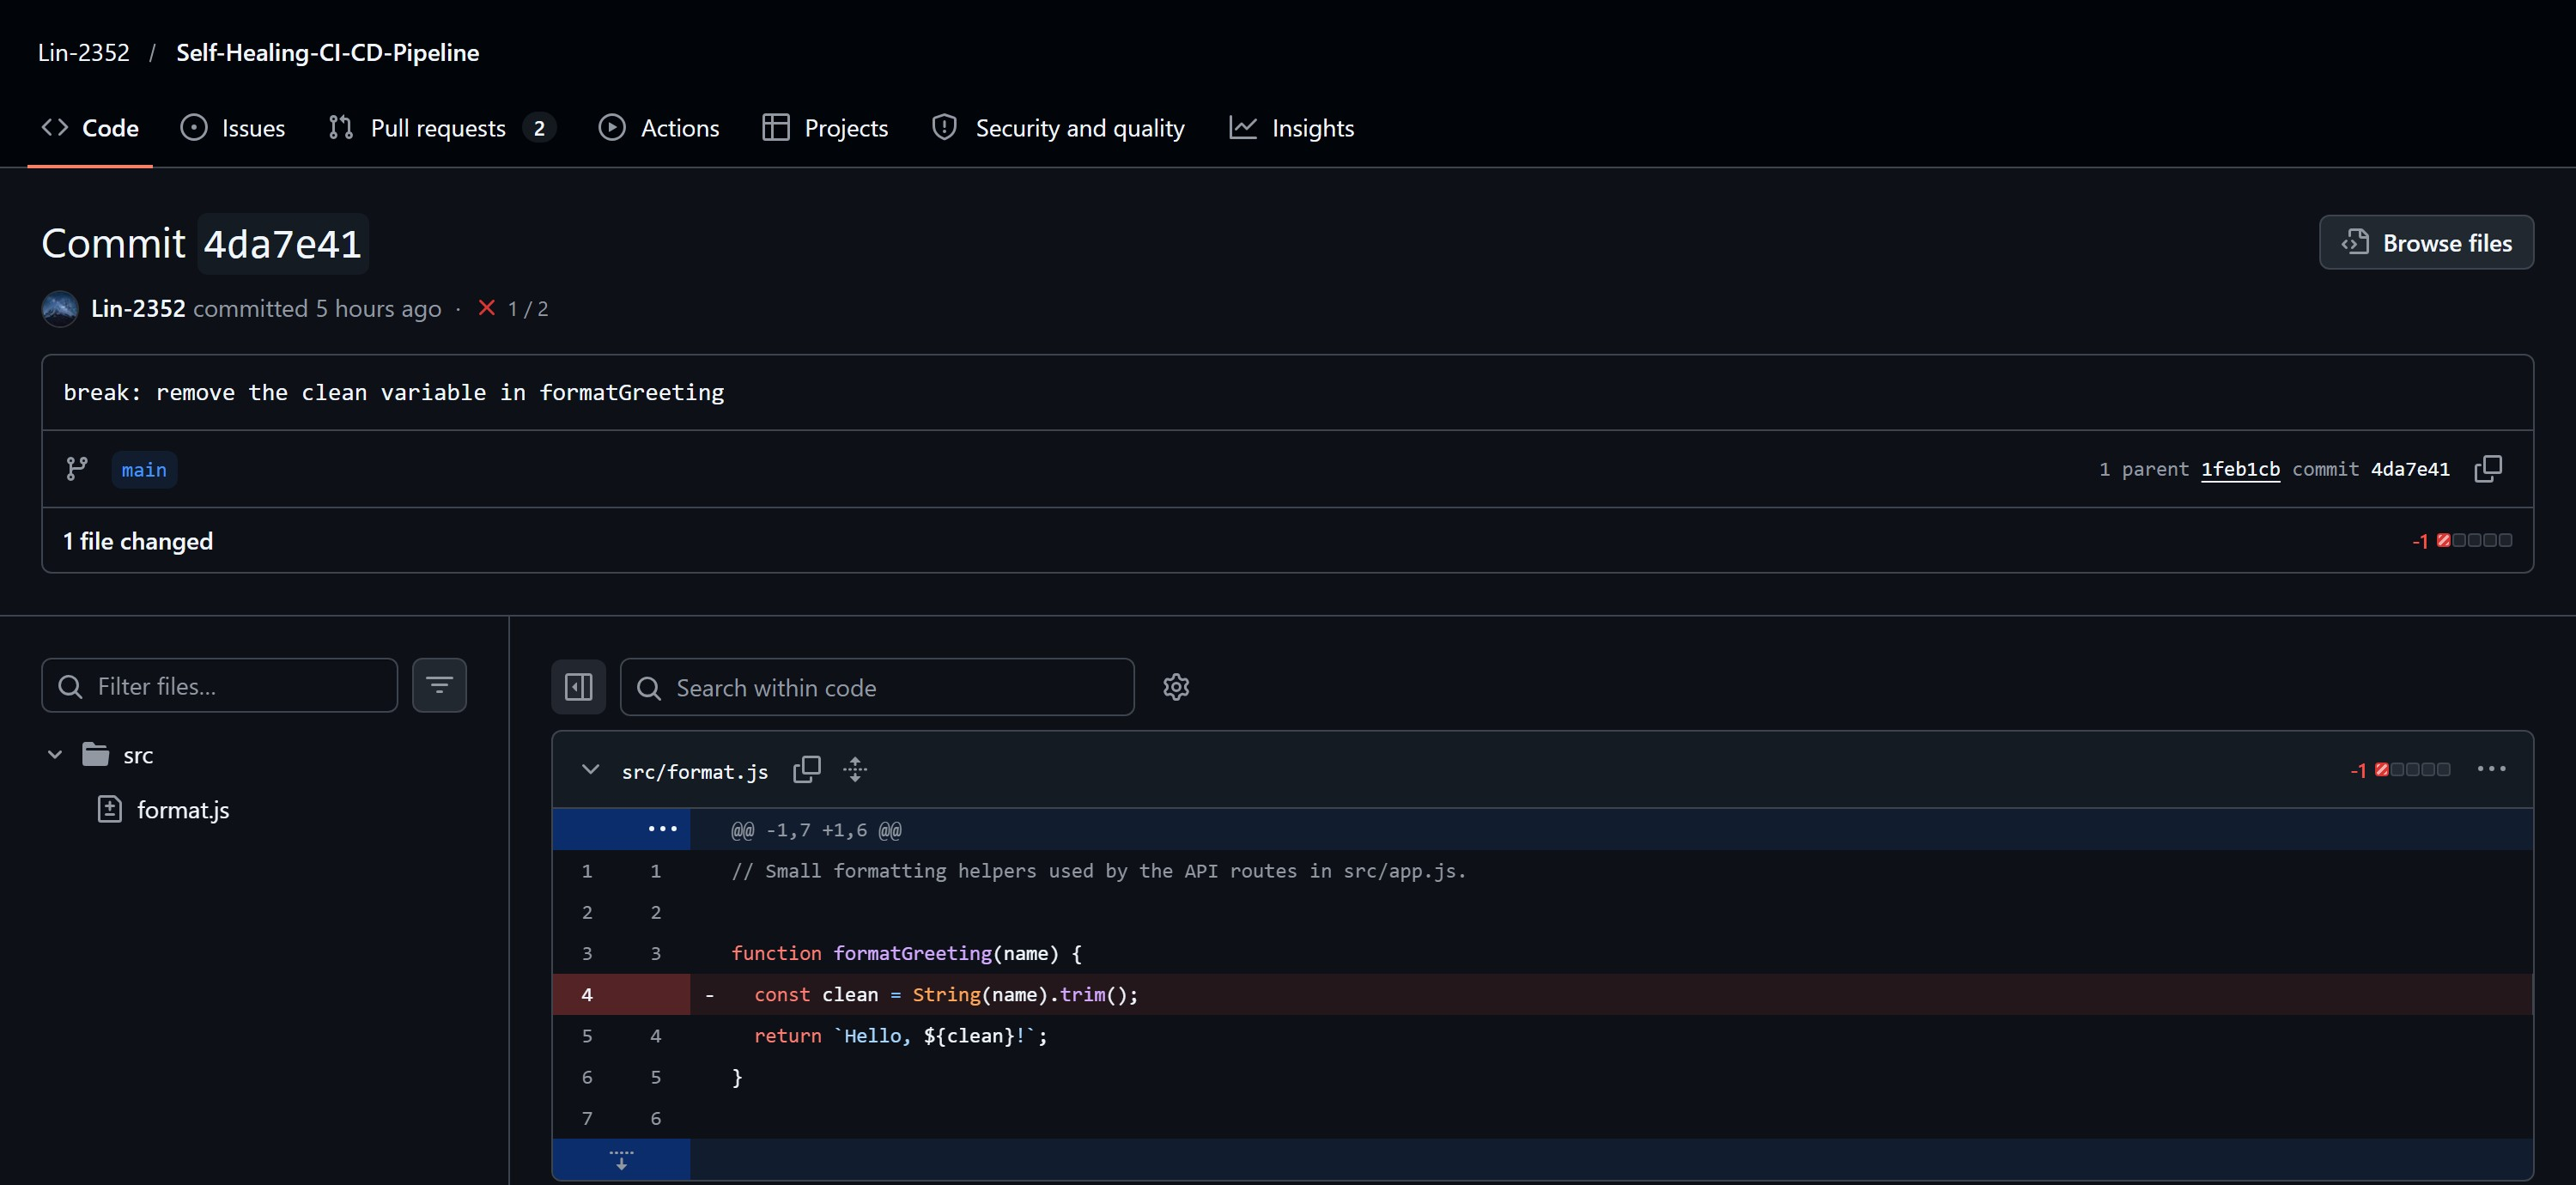
\includegraphics[width=\linewidth]{figures/shots/hq_commit.jpg}
\caption{The breaking commit \texttt{4da7e41}: one line is deleted from \texttt{src/format.js}.}
\label{fig:shot-commit}
\end{figure}
\begin{figure}[!htbp]
\centering
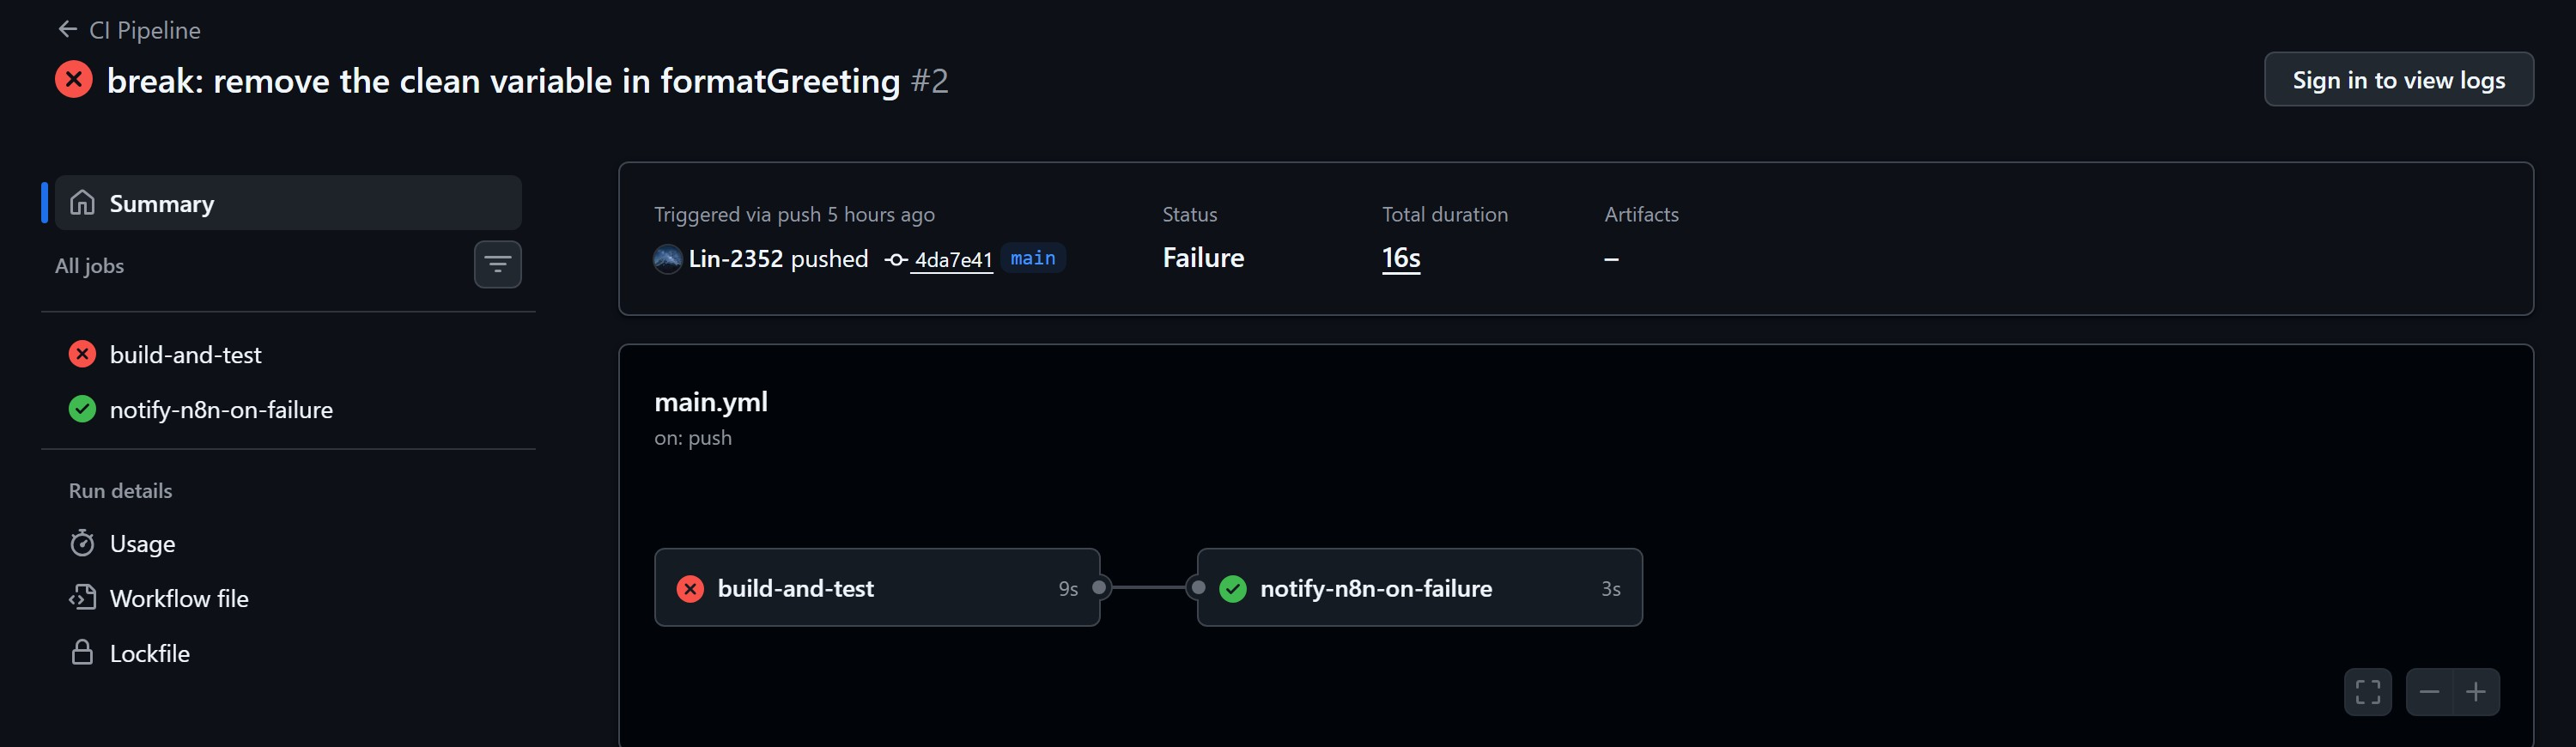
\includegraphics[width=\linewidth]{figures/shots/hq_run.jpg}
\caption{The failing run: \texttt{build-and-test} fails after 9 s, and the \texttt{notify} job that calls n8n passes.}
\label{fig:shot-failed-run}
\end{figure}
\begin{figure}[!htbp]
\centering
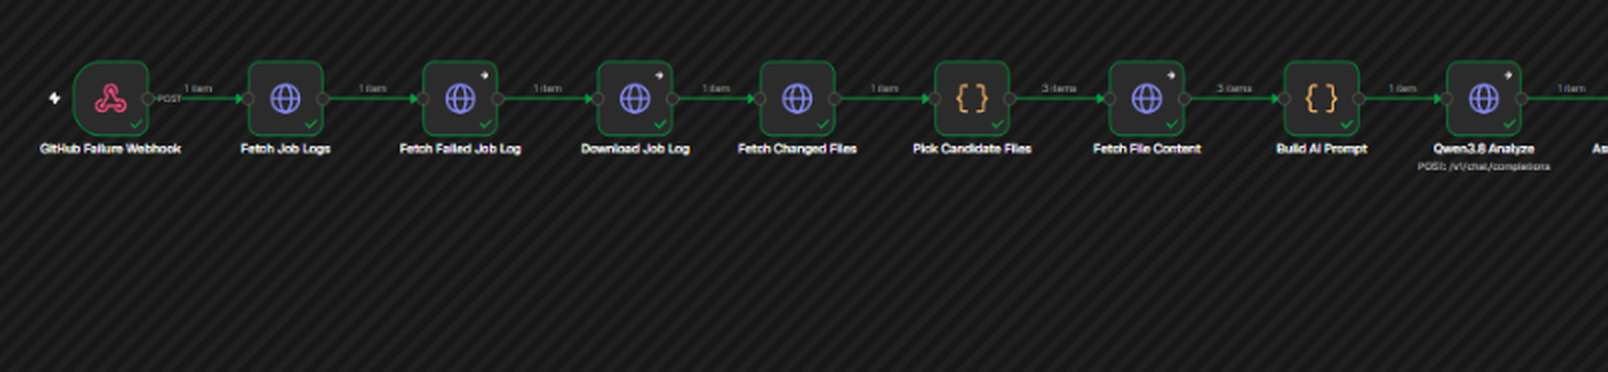
\includegraphics[width=\linewidth]{figures/shots/06a_n8n_left.png}\\[4pt]
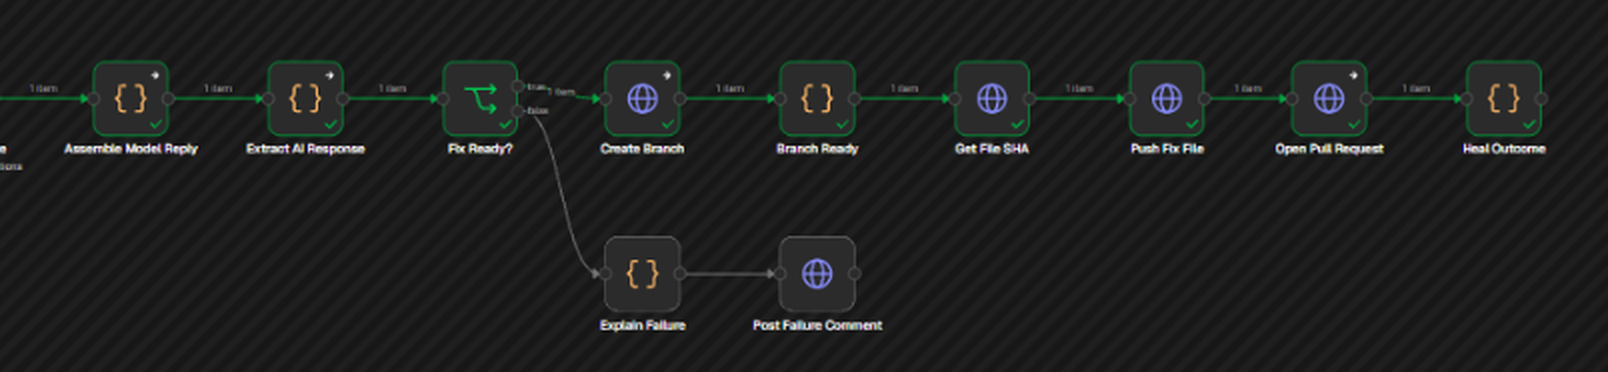
\includegraphics[width=\linewidth]{figures/shots/06b_n8n_right.png}
\caption{The n8n execution of the same run, shown in two halves: every node finished green in 18.7 s.}
\label{fig:shot-n8n}
\end{figure}
\begin{figure}[!htbp]
\centering
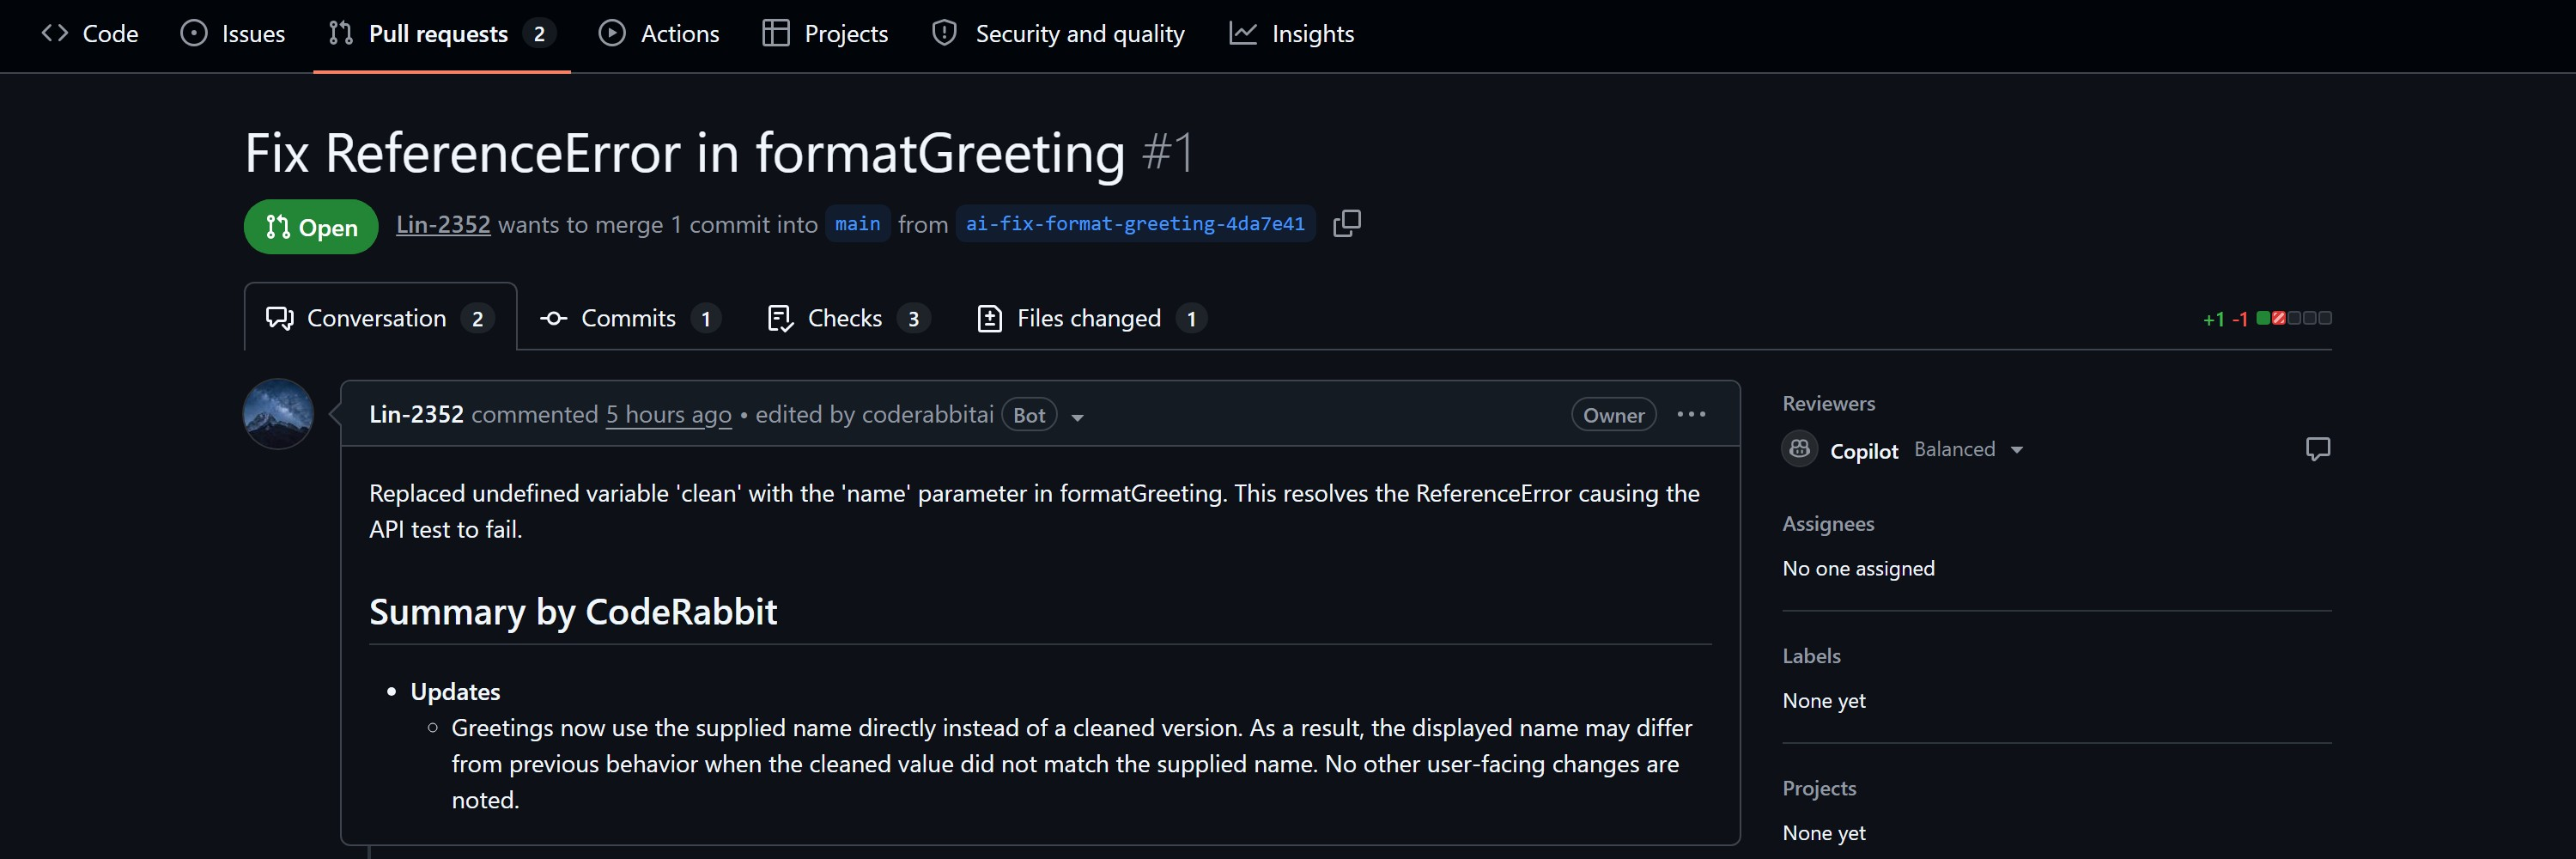
\includegraphics[width=\linewidth]{figures/shots/hq_pr.jpg}
\caption{The pull request opened by the workflow from the branch \texttt{ai-fix-format-greeting-4da7e41}.}
\label{fig:shot-pr}
\end{figure}
\begin{figure}[!htbp]
\centering
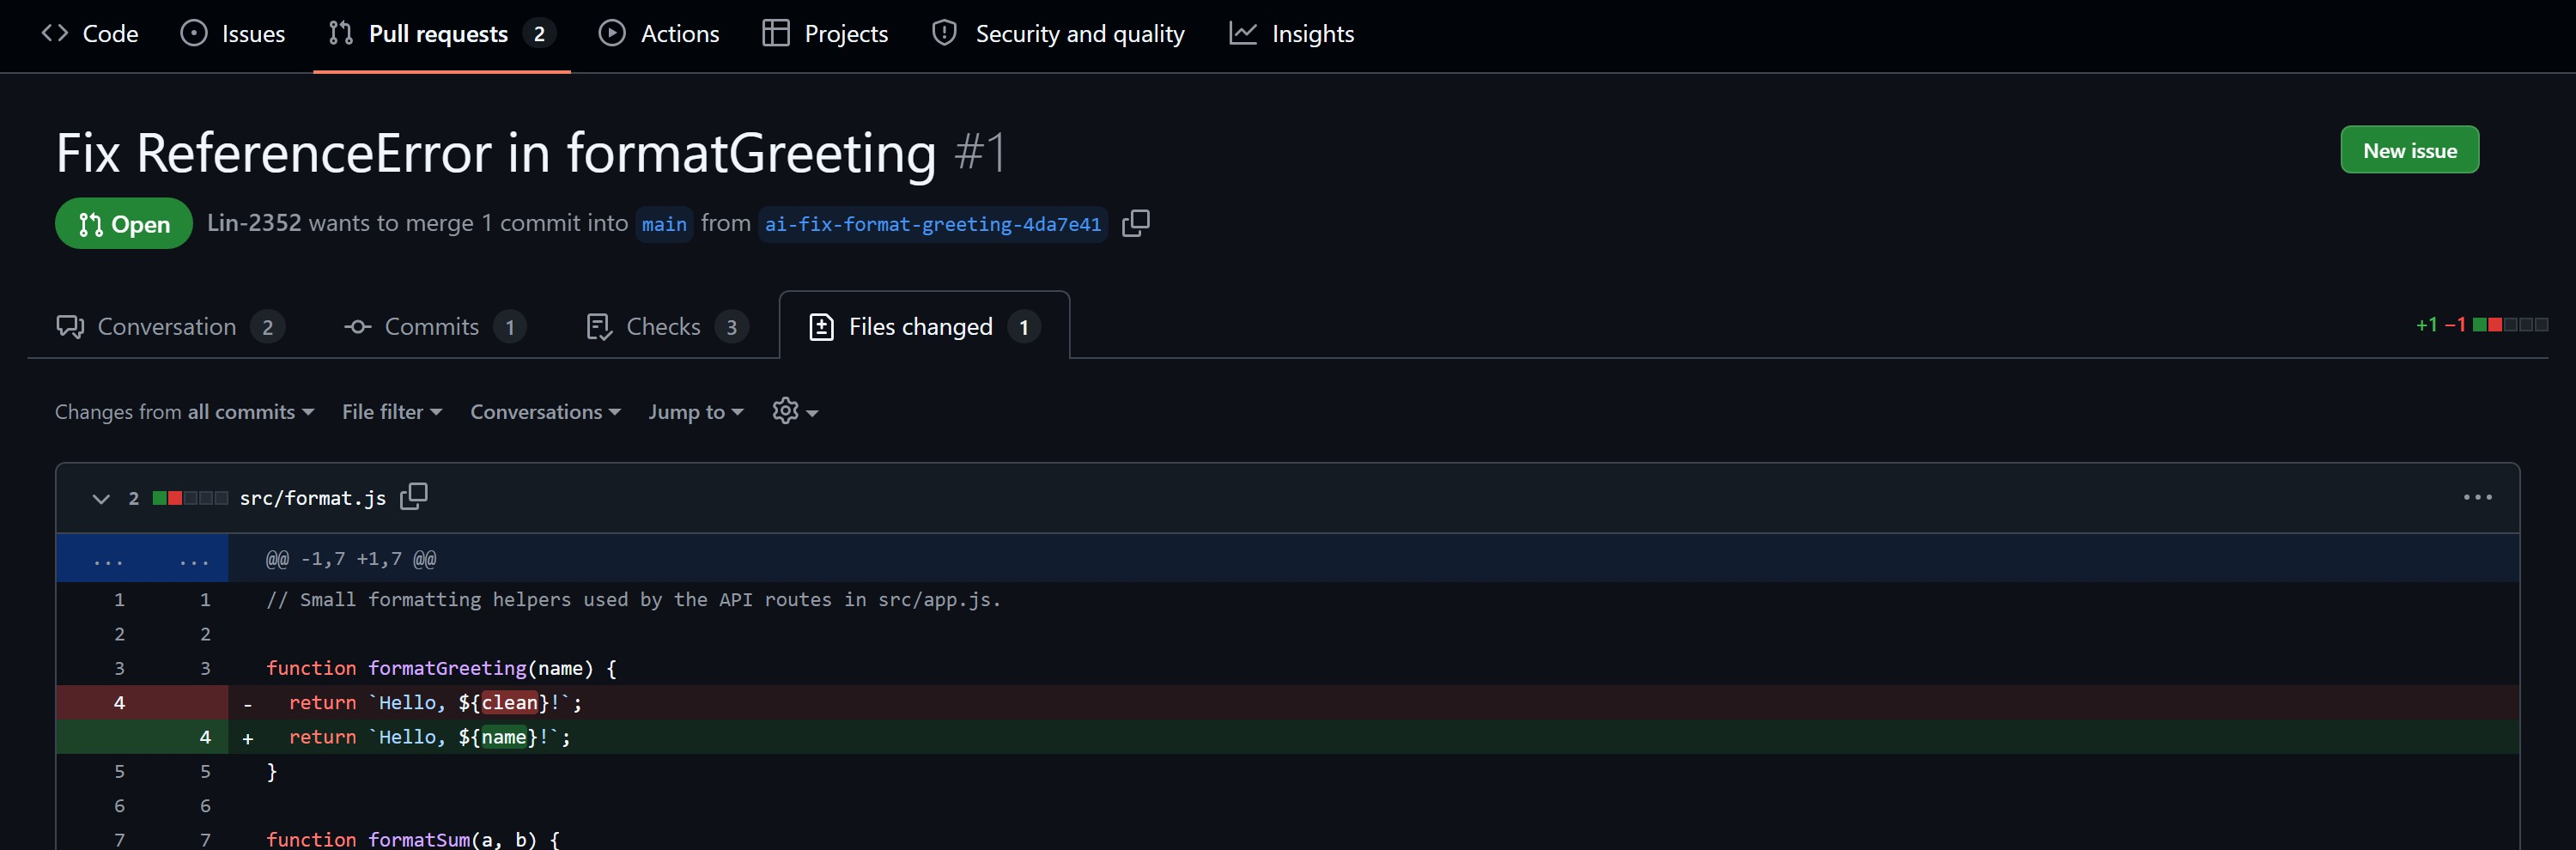
\includegraphics[width=\linewidth]{figures/shots/hq_pr_files.jpg}
\caption{The diff of the pull request: \texttt{\$\{clean\}} becomes \texttt{\$\{name\}}.}
\label{fig:shot-diff}
\end{figure}
\begin{figure}[!htbp]
\centering
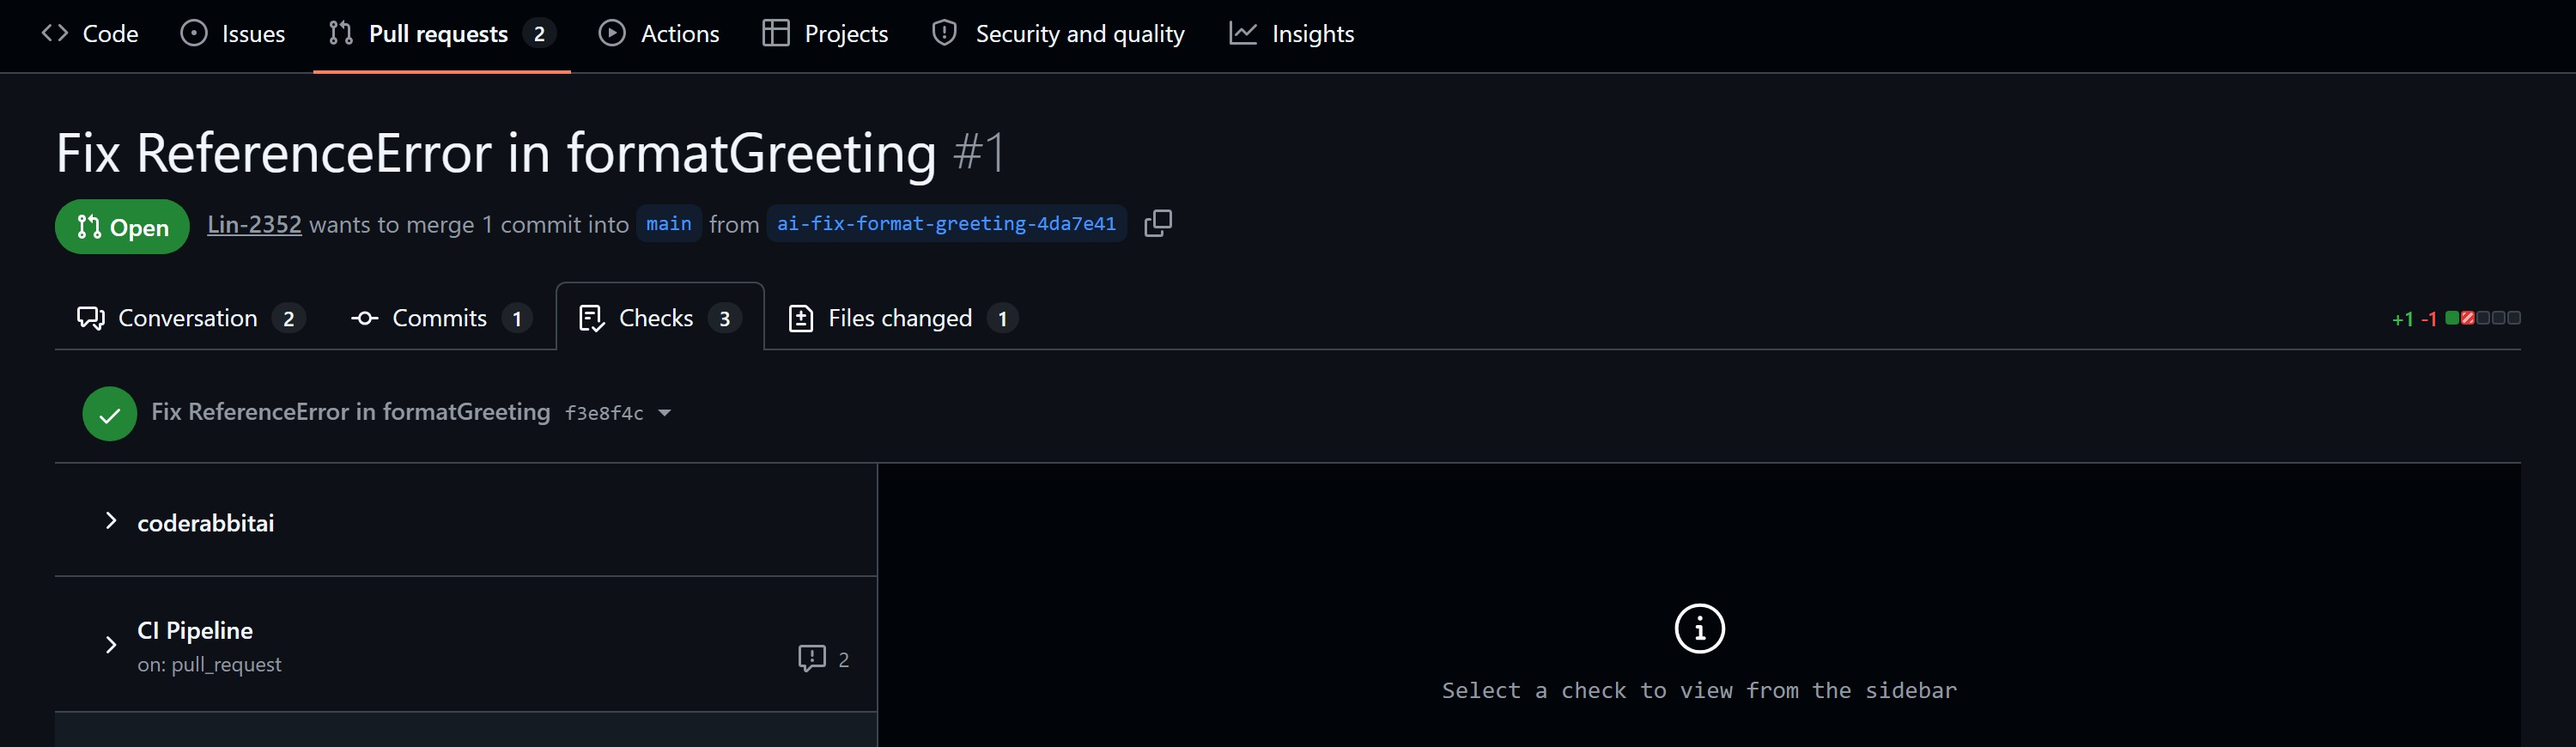
\includegraphics[width=\linewidth]{figures/shots/hq_pr_checks.jpg}
\caption{The checks of the pull request: CI on the fix passes.}
\label{fig:shot-checks}
\end{figure}


\begingroup\small
\begin{longtable}{>{\raggedright\arraybackslash}p{0.071\dimexpr\linewidth-6\tabcolsep\relax}>{\raggedright\arraybackslash}p{0.426\dimexpr\linewidth-6\tabcolsep\relax}>{\raggedright\arraybackslash}p{0.504\dimexpr\linewidth-6\tabcolsep\relax}}
\toprule
\rowcolor{gray!14}\textbf{step} & \textbf{observed} & \textbf{evidence} \\
\midrule
\endhead
\bottomrule
\endfoot
\endlastfoot
1 & The push to \texttt{main} started the workflow run "CI Pipeline \#2". & docs/\allowbreak{}media/\allowbreak{}shots/\allowbreak{}02\_\allowbreak{}actions\_\allowbreak{}runs.jpg \\
2 & \texttt{build-\allowbreak{}and-\allowbreak{}test} failed after 9 s; the run took 16 s in total. The \texttt{notify-\allowbreak{}n8n-\allowbreak{}on-\allowbreak{}failure} job ran and passed after 3 s. & 03\_\allowbreak{}failed\_\allowbreak{}run.jpg \\
3 & The step log shows \texttt{ReferenceError:\allowbreak{} clean is not defined} at \texttt{src/\allowbreak{}format.\allowbreak{}js:\allowbreak{}4:\allowbreak{}20}, then an API test failure, then the line \texttt{npm test exited 1 -\allowbreak{}\textgreater{} failure\_\allowbreak{}kind=code}. & 04\_\allowbreak{}failed\_\allowbreak{}job\_\allowbreak{}log.jpg \\
4 & n8n execution 2 started at 20:45:04, ran 18.699 s and finished with every node green, including all of the branch, push and pull-request nodes. & 05\_\allowbreak{}n8n\_\allowbreak{}execution.jpg, 06\_\allowbreak{}n8n\_\allowbreak{}execution\_\allowbreak{}zoom.png \\
5 & Pull request \#1 "Fix ReferenceError in formatGreeting" opened from the branch \texttt{ai-\allowbreak{}fix-\allowbreak{}format-\allowbreak{}greeting-\allowbreak{}4da7e41} (commit \texttt{f3e8f4c}). & 07\_\allowbreak{}pr\_\allowbreak{}conversation.jpg \\
6 & The diff changes one line: \texttt{\$\{clean\}} becomes \texttt{\$\{name\}}. & 08\_\allowbreak{}pr\_\allowbreak{}diff.jpg \\
7 & CI on the pull request ran 12 s and passed. & 09\_\allowbreak{}pr\_\allowbreak{}checks.jpg, run "CI Pipeline \#3" \\
\bottomrule
\caption{What happened}\label{tab:09arecor-1}\\
\end{longtable}
\endgroup

The breaking commit was pushed at 8:44 PM and the fix pull request's own CI run is listed at 8:45 PM, so the whole chain from push to a passing fix pull request took about a minute on GitHub's minute-resolution timestamps. The two intervals that the pages report to the second are the n8n execution (18.7 s) and the CI run of the fix (12 s).

\subsection{What the run does not show}

The fix is not the original code. The deleted line also converted the value to a string and trimmed it; the model's edit replaces the variable with the raw parameter, so the tests pass while the trimming behaviour is gone. The pipeline's own gates (the SEARCH text matches once, the file parses, CI passes) cannot detect this, which is why the result is a pull request for a person to review, not a merge.

The run used the n8n workflow as it stood before the fallback nodes were added (the execution canvas shows 20 nodes). Later runs on the same repository the same evening used the 26-node version: a run with the model address deliberately set to a dead host went through the OpenAI fallback node, which answered \texttt{Forbidden} (n8n's included free credits did not work for that webhook-triggered run; the cause was not established), and a run after the model address was stored through the Set Model URL webhook healed through Qwen and opened pull request \#2 (execution 6, 17.886 s). The fallback routing is verified by the real-engine tests in Chapter 11; a fix produced by OpenAI has never been observed.

\subsection{A run that could not be repeated}

A second live run for this report was started on 2026-11-15: version 18 of the Kaggle endpoint notebook was pushed and then stayed in the Kaggle queue for about an hour and a half without receiving a GPU. It was cancelled, and the recording above was built from the earlier run, whose pages are still on GitHub and in n8n. Availability of the free GPU is a real operating constraint (Chapter 13).

% GENERATED by build_chapters.py; edit docs/report/chapters, not this file

\chapter{Security, Testing and Deployment}

\section{Security}

A pipeline that reads logs written by anyone who can push code, sends them to a model, and then writes to a repository has three things to protect: its credentials, the repository, and its own decisions. This chapter lists what is protected and how, and ends with the weaknesses that are known and open.

\subsection{Credentials}

\begingroup\small
\begin{longtable}{>{\raggedright\arraybackslash}p{0.165\dimexpr\linewidth-6\tabcolsep\relax}>{\raggedright\arraybackslash}p{0.457\dimexpr\linewidth-6\tabcolsep\relax}>{\raggedright\arraybackslash}p{0.378\dimexpr\linewidth-6\tabcolsep\relax}}
\toprule
\textbf{secret} & \textbf{where it lives} & \textbf{who can read it} \\
\midrule
\endhead
\bottomrule
\endfoot
\endlastfoot
Webhook shared secret & the n8n credential "N8N Webhook Secret" (header auth, header \texttt{X-\allowbreak{}Webhook-\allowbreak{}Secret}), the GitHub repository secret \texttt{N8N\_\allowbreak{}WEBHOOK\_\allowbreak{}SECRET}, and \texttt{secrets.\allowbreak{}json} on the operator's PC & the workflow, the notify job and the launcher scripts \\
GitHub token & the n8n credential "GitHub PAT" (bearer); locally taken from the GitHub CLI by \texttt{tools/\allowbreak{}golive/\allowbreak{}n8n\_\allowbreak{}import.\allowbreak{}py} & the n8n HTTP nodes that call the GitHub API \\
Model endpoint key & the n8n credential "Qwen3.8 Endpoint Key" and the constant \texttt{API\_\allowbreak{}KEY} in \texttt{kaggle/\allowbreak{}endpoint/\allowbreak{}deploy\_\allowbreak{}src.\allowbreak{}py} & anyone who can read the repository \\
Webhook address & the repository secret \texttt{N8N\_\allowbreak{}WEBHOOK\_\allowbreak{}URL} & the notify job \\
\bottomrule
\caption{Credentials}\label{tab:10securi-1}\\
\end{longtable}
\endgroup

Runtime secrets (\texttt{secrets.\allowbreak{}json}, the saved model address) live under \texttt{\%LOCALAPPDATA\%\textbackslash{}selfheal-\allowbreak{}n8n\textbackslash{}}, outside the repository. The backend's \texttt{.\allowbreak{}env} is ignored by git. The repository contains no token strings; this is checked by \texttt{tools/\allowbreak{}tests/\allowbreak{}test\_\allowbreak{}workflow\_\allowbreak{}structure.\allowbreak{}py} for the workflow JSON, and by a search of the whole tree before each push (see below). Credentials are imported into a local n8n as a plaintext file that the import script deletes immediately afterwards (tools/\allowbreak{}golive/\allowbreak{}n8n\_\allowbreak{}import.py).

\subsection{The webhooks}

Both n8n webhooks require the shared secret as a header and n8n rejects a request without it before the workflow starts: a wrong secret gave HTTP 403 in a test against the cloud instance, and the right one started the workflow. The second webhook, which stores the model address, accepts only an address that matches \texttt{https:\allowbreak{}/\allowbreak{}/\allowbreak{}\textless{}letters, digits, hyphens\textgreater{}.\allowbreak{}trycloudflare.\allowbreak{}com} and keeps the old address otherwise (tools/\allowbreak{}nodes/\allowbreak{}store\_\allowbreak{}model\_\allowbreak{}url.js, tested in tools/\allowbreak{}tests/\allowbreak{}test\_\allowbreak{}model\_\allowbreak{}url.py with look-alike hosts such as \texttt{https:\allowbreak{}/\allowbreak{}/\allowbreak{}abc.\allowbreak{}trycloudflare.\allowbreak{}com.\allowbreak{}evil.\allowbreak{}com}). A stolen secret could therefore still point the workflow at an attacker's tunnel, which is one reason to keep the secret long and to rotate it.

\texttt{ci-\allowbreak{}heal-\allowbreak{}backend} verifies GitHub's HMAC-SHA256 signature on the raw body with a constant-time comparison, applies a repository allowlist that denies by default, protects its operator API with a token outside development, and now ignores runs from fork pull requests and refuses to start outside \texttt{dev} with an empty or placeholder secret (docs/\allowbreak{}results/\allowbreak{}BACKEND\_\allowbreak{}AUDIT.md).

\subsection{The log redirect}

The job-log endpoint of the GitHub API answers with a redirect to a signed address on another host. n8n re-sends the credential's authorization header when it follows a redirect, which would hand the GitHub token to the storage host. The workflow therefore does not follow the redirect: one node reads the address from the 302 answer, and a second node without any credential downloads it. The real-engine rig checks this: the token reaches the API host and does not reach the blob host (tools/\allowbreak{}n8n\_\allowbreak{}rig/\allowbreak{}drive\_\allowbreak{}full.py, eval/\allowbreak{}runs/\allowbreak{}testall/\allowbreak{}n8n\_\allowbreak{}rig.txt).

\subsection{Treating the model as untrusted}

The prompt contains text written by whoever caused the failure: log lines, file contents. The design assumes the model may be steered by that text or may simply be wrong, so every step after the reply is a gate.

\begin{itemize}[leftmargin=*, itemsep=2pt]
\item Only failures marked \texttt{failure\_\allowbreak{}kind=code} reach the model, and a payload with any other kind is refused inside the workflow as well (tools/\allowbreak{}nodes/\allowbreak{}build\_\allowbreak{}ai\_\allowbreak{}prompt.js).
\item The reply must be a JSON object with SEARCH/\allowbreak{}REPLACE edits. Each SEARCH text must occur in the file exactly once, and the result must parse as JavaScript (tools/\allowbreak{}nodes/\allowbreak{}extract\_\allowbreak{}ai\_\allowbreak{}response.js).
\item The file the edit names must be one of the files the model was shown.
\item A branch named \texttt{main} or \texttt{master} is replaced by an \texttt{ai-\allowbreak{}fix-\allowbreak{}} name, and the fix is a pull request, never a push to the main branch.
\item CI runs on the pull request, and a person merges it.
\item The backend adds secret redaction before any text reaches a model, caps on edit size, a check against weakened tests, and an \texttt{ai-\allowbreak{}fix-\allowbreak{}} prefix rule enforced in the GitHub client (ci-heal-backend/\allowbreak{}app/\allowbreak{}services/\allowbreak{}github\_\allowbreak{}client.py, \texttt{\_\allowbreak{}refuse}).
\end{itemize}

\subsection{Known weaknesses}

\begin{itemize}[leftmargin=*, itemsep=2pt]
\item \textbf{The endpoint key is public.} It is a constant in a file in the repository. Anyone who reads the repository and learns the tunnel address can use the GPU session. The address changes on every boot and is not published, which limits the exposure but is not authentication.
\item \textbf{The shared secret in use is short.} It was chosen for convenience and should be replaced by a long random value before the repository or its secrets are shared.
\item \textbf{A misled fix is still a candidate.} A log line that argues for a particular edit can influence the model. The gates above stop a malformed or unrelated edit, not a plausible wrong one that happens to pass the tests. The review of the pull request is the control.
\item \textbf{Pull-request CI runs the proposed code.} The fix pull request is built by the repository's own workflow, with whatever that workflow can access. The audit of the backend noted that only workflow files, \texttt{.\allowbreak{}git} and \texttt{.\allowbreak{}env} files are blocked from editing, so a build entry point such as \texttt{package.\allowbreak{}json} can be changed by a fix.
\item \textbf{Seven workflow nodes have no error setting}, so a failure there ends the run silently (Chapter 11). Seventeen backend findings are open (docs/\allowbreak{}results/\allowbreak{}BACKEND\_\allowbreak{}AUDIT.md).
\item \textbf{The backend reads a webhook body in full} before it checks the size limit and the signature (finding 11 in docs/\allowbreak{}results/\allowbreak{}BACKEND\_\allowbreak{}AUDIT.md).
\end{itemize}

\subsection{Checks before publishing}

Before each push the tree is searched for the token prefixes \texttt{ghp\_\allowbreak{}} and \texttt{github\_\allowbreak{}pat\_\allowbreak{}}, for \texttt{hf\_\allowbreak{}}, for the webhook secret value, and for \texttt{.\allowbreak{}env} and \texttt{secrets.\allowbreak{}json} files. A match in a test that deliberately contains a fake token is accepted after reading it.

\section{Testing and Verification}

The project has four layers of checks, from fast and local to slow and live. The first three need no GPU and write nothing to GitHub. A fuller guide with commands is in docs/\allowbreak{}guides/\allowbreak{}testing.md.

\subsection{Layer 1: backend unit tests}

\texttt{ci-\allowbreak{}heal-\allowbreak{}backend} has a pytest suite that uses a mock model and a mocked GitHub client, so it needs no key and no network. It collected 157 tests before the audit fixes described in Chapter 8 and 205 after, all passing, with \texttt{ruff check .\allowbreak{}} and \texttt{ruff format -\allowbreak{}-\allowbreak{}check .\allowbreak{}} clean (run on 2026-11-15, output recorded in docs/\allowbreak{}results/\allowbreak{}BACKEND\_\allowbreak{}AUDIT.md). The suite covers the classifier, the decision rules, patch application, the HTTP model client, the GitHub client, both webhooks, secret redaction, log trimming, the database layer and the settings.

\subsection{Layer 2: node suites and eval scorers}

\texttt{python run\_\allowbreak{}tests.\allowbreak{}py} runs every suite in \texttt{tools/\allowbreak{}tests/\allowbreak{}}, the scorer self-tests in \texttt{eval/\allowbreak{}} and a generator check. Each Code node of the n8n workflow is a plain JavaScript file, so \texttt{tools/\allowbreak{}heal\_\allowbreak{}harness.\allowbreak{}py} can run it under Node with a fake n8n context. The table gives the number of passing assertions each suite printed in its last run (eval/\allowbreak{}runs/\allowbreak{}testall/\allowbreak{}).

\begingroup\small
\begin{longtable}{>{\raggedright\arraybackslash}p{0.397\dimexpr\linewidth-6\tabcolsep\relax}>{\raggedright\arraybackslash}p{0.190\dimexpr\linewidth-6\tabcolsep\relax}>{\raggedright\arraybackslash}p{0.414\dimexpr\linewidth-6\tabcolsep\relax}}
\toprule
\textbf{suite} & \textbf{passing assertions} & \textbf{what it checks} \\
\midrule
\endhead
\bottomrule
\endfoot
\endlastfoot
test\_\allowbreak{}build\_\allowbreak{}prompt & 29 & the prompt carries the trimmed CI error and the shipped system prompt \\
test\_\allowbreak{}extract\_\allowbreak{}node & 15 & SEARCH/\allowbreak{}REPLACE application and every rejection reason \\
test\_\allowbreak{}assemble\_\allowbreak{}reply & 15 & rebuilding a streamed reply, and the failure explanation \\
test\_\allowbreak{}heal\_\allowbreak{}outcome & 6 & the retry outcome against GitHub error bodies \\
test\_\allowbreak{}model\_\allowbreak{}url & 30 & storing and reading the model address, and the fallback reply \\
test\_\allowbreak{}multifile & 19 & candidate file choice and prompt for multi-file bugs \\
test\_\allowbreak{}workflow\_\allowbreak{}structure & 22 & wiring, webhooks and credentials of the shipped workflow JSON \\
test\_\allowbreak{}shipped\_\allowbreak{}eval & 49 & the scorer of the quality study, including 15 of 15 real captured replies \\
check\_\allowbreak{}multifile\_\allowbreak{}cases & 7 & every multi-file case is a real test: golden passes, broken fails \\
test\_\allowbreak{}multifile\_\allowbreak{}eval & 13 & scoring of the multi-file study \\
test\_\allowbreak{}bakeoff\_\allowbreak{}eval & 52 & the bake-off kernel's functions and decision rule \\
\bottomrule
\caption{Layer 2: node suites and eval scorers}\label{tab:10testin-1}\\
\end{longtable}
\endgroup

The generator check regenerates \texttt{n8n/\allowbreak{}self\_\allowbreak{}healing\_\allowbreak{}pipeline.\allowbreak{}json} from \texttt{tools/\allowbreak{}gen\_\allowbreak{}n8n.\allowbreak{}py} and the node files and requires a byte-identical result, so the file in the repository cannot drift from its source. In the last full run all 13 checks passed (12 without the rig, 13 with it).

The harness has a known blind spot, stated in its own docstring: it resolves \texttt{\$('Node')} lookups that n8n's sandbox does not resolve for Code nodes. A passing harness run therefore does not prove that an accessor works in n8n. This is the reason for layer 3.

\subsection{Layer 3: a real n8n engine}

\texttt{python run\_\allowbreak{}tests.\allowbreak{}py -\allowbreak{}-\allowbreak{}rig} imports the workflow nodes into a real n8n 1.x and runs them against a local mock of GitHub and the model (tools/\allowbreak{}n8n\_\allowbreak{}rig/\allowbreak{}). The nodes under test are the shipped ones, copied from the workflow JSON; only host names are changed and credentials removed. The last run printed 18 passing scenarios and no failures (eval/\allowbreak{}runs/\allowbreak{}testall/\allowbreak{}n8n\_\allowbreak{}rig.txt). They include:

\begin{itemize}[leftmargin=*, itemsep=2pt]
\item the CI log reaches the prompt and the PAT is sent to the GitHub API host but not to the blob host the log redirect points to;
\item the same fix is produced on a first heal, on a retry (thinking on, same branch, trailer \texttt{Heal-\allowbreak{}Attempt:\allowbreak{} 2}) and on a trace-only multi-file bug;
\item each rejection path of the extract node posts a comment on the commit that quotes its reason;
\item a model call that times out with HTTP 524 and a fallback that also fails ends in a pull-request comment that names both causes;
\item a model call that times out and a fallback that answers still produces the correct fix and no comment;
\item a job log that returns 404 still heals with the text \texttt{(log unavailable)};
\item a payload with hostile characters still builds a valid request;
\item a payload with \texttt{failure\_\allowbreak{}kind=infra} is refused before any model call.
\end{itemize}

\subsection{Layer 4: live runs}

Live runs push a deliberately broken commit to a GitHub repository and watch the whole chain, with the real model on Kaggle. They are run by hand because they write to GitHub and use GPU quota. Chapter 9 and Chapter 10 report them.

\subsection{Audit}

A read-only security and reliability review of \texttt{ci-\allowbreak{}heal-\allowbreak{}backend} listed 21 findings. Four were fixed with tests that failed first, and 17 are open (docs/\allowbreak{}results/\allowbreak{}BACKEND\_\allowbreak{}AUDIT.md). The n8n workflow was reviewed by reading its nodes against the tests: seven nodes (Fetch Job Logs, Fetch Changed Files, Build AI Prompt, Get Model URL, Get File SHA, Push Fix File and Post Failure Comment) have no error setting, so a failure there ends the execution without a comment on GitHub (docs/\allowbreak{}architecture/\allowbreak{}n8n-workflow.md).

\subsection{What is not tested}

\begin{itemize}[leftmargin=*, itemsep=2pt]
\item \texttt{kaggle/\allowbreak{}endpoint/\allowbreak{}deploy\_\allowbreak{}src.\allowbreak{}py} runs only on a Kaggle GPU; its test is a real boot.
\item The GitHub write steps of the workflow, from branch creation to the pull request, run only in live runs.
\item The backend with \texttt{DRY\_\allowbreak{}RUN=false} against real GitHub has no automated test.
\item The OpenAI fallback node is tested for wiring, for shipping without a credential and for its error handling, but never against a real OpenAI account. On the n8n Cloud trial the included free credits answered \texttt{Forbidden} to a webhook-triggered run in our test (docs/\allowbreak{}guides/\allowbreak{}cloud-n8n.md).
\item \texttt{demo-\allowbreak{}ci.\allowbreak{}yml} is exercised only by pushing to GitHub.
\item The launcher scripts have no tests.
\end{itemize}

\section{Deployment and Operation}

The launcher folder holds double-click scripts for every step, so nobody has to remember the command lines (launcher/\allowbreak{}README.md). This chapter lists what runs where, the order to start things in, and what each step costs.

\subsection{What runs where}

\begingroup\small
\begin{longtable}{>{\raggedright\arraybackslash}p{0.163\dimexpr\linewidth-8\tabcolsep\relax}>{\raggedright\arraybackslash}p{0.153\dimexpr\linewidth-8\tabcolsep\relax}>{\raggedright\arraybackslash}p{0.432\dimexpr\linewidth-8\tabcolsep\relax}>{\raggedright\arraybackslash}p{0.253\dimexpr\linewidth-8\tabcolsep\relax}}
\toprule
\textbf{part} & \textbf{runs on} & \textbf{started by} & \textbf{stopped by} \\
\midrule
\endhead
\bottomrule
\endfoot
\endlastfoot
Qwen3.8-27B endpoint & Kaggle, 2 x T4 & \texttt{launcher/\allowbreak{}start/\allowbreak{}1\_\allowbreak{}start\_\allowbreak{}model\_\allowbreak{}on\_\allowbreak{}kaggle.\allowbreak{}bat} & Stop Session in the Kaggle page (the Kaggle command line cannot stop a session) \\
n8n workflow, cloud copy & n8n Cloud trial, always on & already published & unpublish in the editor \\
n8n workflow, local copy & this PC, \texttt{localhost:\allowbreak{}5678} & \texttt{start/\allowbreak{}start\_\allowbreak{}n8n\_\allowbreak{}local\_\allowbreak{}only.\allowbreak{}bat}, or \texttt{2\_\allowbreak{}} and \texttt{3\_\allowbreak{}} for the live setup & \texttt{end/\allowbreak{}stop\_\allowbreak{}n8n.\allowbreak{}bat} \\
ci-heal-backend & this PC, port 8000 & \texttt{start/\allowbreak{}4\_\allowbreak{}start\_\allowbreak{}backend.\allowbreak{}bat} & \texttt{end/\allowbreak{}stop\_\allowbreak{}backend.\allowbreak{}bat} \\
demo repository workflow & GitHub Actions & a push to \texttt{main} that changes \texttt{demo-\allowbreak{}app/\allowbreak{}} & not applicable \\
\bottomrule
\caption{What runs where}\label{tab:10deploy-1}\\
\end{longtable}
\endgroup

\subsection{The live demo in order}

\begin{enumerate}[leftmargin=*, itemsep=2pt]
\item \texttt{1\_\allowbreak{}start\_\allowbreak{}model\_\allowbreak{}on\_\allowbreak{}kaggle.\allowbreak{}bat}. It prints the status of the project's kernels, builds the endpoint notebook from \texttt{kaggle/\allowbreak{}endpoint/\allowbreak{}deploy\_\allowbreak{}src.\allowbreak{}py}, pushes it, follows the boot log for about four minutes, saves the tunnel address to \texttt{\%LOCALAPPDATA\%\textbackslash{}selfheal-\allowbreak{}n8n\textbackslash{}qwen\_\allowbreak{}url.\allowbreak{}txt} and posts it to the cloud workflow's Set Model URL webhook.
\item Push a commit that breaks a test in \texttt{demo-\allowbreak{}app/\allowbreak{}}. The Actions run fails, the notify job posts to the n8n webhook, and a pull request on an \texttt{ai-\allowbreak{}fix-\allowbreak{}.\allowbreak{}.\allowbreak{}.\allowbreak{}} branch appears about a minute later.
\item Stop the Kaggle session when finished, either with \texttt{end/\allowbreak{}stop\_\allowbreak{}model\_\allowbreak{}on\_\allowbreak{}kaggle.\allowbreak{}bat} (it opens the notebook page and then checks that the session stopped) or directly in the page: View Active Events, the three-dot menu on the session, Stop Session.
\end{enumerate}

For the local copy of n8n instead of the cloud one, run \texttt{2\_\allowbreak{}load\_\allowbreak{}workflow\_\allowbreak{}into\_\allowbreak{}n8n.\allowbreak{}bat} and \texttt{3\_\allowbreak{}start\_\allowbreak{}n8n\_\allowbreak{}live.\allowbreak{}bat} after step 1. The second imports the workflow and credentials with the current model address, and the third starts n8n with a public Cloudflare tunnel and points the repository's \texttt{N8N\_\allowbreak{}WEBHOOK\_\allowbreak{}URL} secret at it.

\subsection{Cost and limits}

The Kaggle session uses GPU quota for as long as it runs. The kernel stops itself after 1.5 hours (kaggle/\allowbreak{}endpoint/\allowbreak{}deploy\_\allowbreak{}src.py, \texttt{HOURS}), and \texttt{push.\allowbreak{}py} refuses to start a second session while one is running or queued. A boot took about four minutes in the logged runs, with the model download taking 76 to 91 seconds (kaggle/\allowbreak{}logs/\allowbreak{}endpoint/\allowbreak{}). A pushed version that is stopped before it finishes does not become the notebook's default view on the Kaggle page; pinning it as the default version in the version history does (observed on the Kaggle page, 2026-11-15).

The n8n Cloud instance is a 14-day trial. After it ends the same workflow can be imported into a local n8n 1.x, which is what the launcher's local scripts do.

\subsection{Troubleshooting}

\begingroup\small
\begin{longtable}{>{\raggedright\arraybackslash}p{0.291\dimexpr\linewidth-6\tabcolsep\relax}>{\raggedright\arraybackslash}p{0.291\dimexpr\linewidth-6\tabcolsep\relax}>{\raggedright\arraybackslash}p{0.418\dimexpr\linewidth-6\tabcolsep\relax}}
\toprule
\textbf{symptom} & \textbf{cause found in practice} & \textbf{action} \\
\midrule
\endhead
\bottomrule
\endfoot
\endlastfoot
The workflow's model call fails right after a Kaggle restart & The tunnel address changed and the workflow still holds the old one & run \texttt{launcher\textbackslash{}start\textbackslash{}show\_\allowbreak{}model\_\allowbreak{}info.\allowbreak{}bat}; run \texttt{python tools\textbackslash{}golive\textbackslash{}set\_\allowbreak{}cloud\_\allowbreak{}qwen\_\allowbreak{}url.\allowbreak{}py} to post the new address \\
Kaggle status stays \texttt{QUEUED} for several minutes & the notebook is waiting for a GPU & wait; \texttt{push.\allowbreak{}py} will refuse a second push in the meantime \\
\texttt{watch\_\allowbreak{}deploy.\allowbreak{}py} prints \texttt{500 Server Error} from the Kaggle log stream & the Kaggle log API failed once & it reconnects by itself; check the status with \texttt{kaggle/\allowbreak{}tools/\allowbreak{}status.\allowbreak{}py} \\
Local n8n starts but the webhook does nothing & n8n 2.x does not register the webhook & install n8n 1.x (docs/\allowbreak{}guides/\allowbreak{}SETUP.md) \\
A fix pull request appears but CI on it is red & the model's fix parsed but was wrong & the retry loop tries again with thinking, up to the attempt cap; after that a comment says a person has to look \\
\bottomrule
\caption{Troubleshooting}\label{tab:10deploy-2}\\
\end{longtable}
\endgroup

\chapter{Standards Adopted}

This chapter lists the standards that the project follows and, for each one, the file or check that keeps it in force. A standard that is only written in a README is called a convention here, and the text says so. Where the repository has no enforcement, the text says that as well.

\section{Design Standards}

\subsection{Webhook and REST conventions}

\textbf{Standard.} A webhook must authenticate its sender before doing any work, answer quickly and do the real work afterwards. Status codes carry the result: 401 for a wrong secret, 403 for a repository that is not allowed, 202 for work that was accepted or deliberately ignored, and 200 for a GitHub \texttt{ping}. The read routes of the API use \texttt{GET}.

\textbf{Where it is enforced.}
\begin{itemize}
  \item \textbf{Backend webhooks:} \texttt{POST /webhooks/github} checks the \texttt{X-Hub-Signature-256} HMAC over the raw body, and \texttt{POST /webhooks/n8n} compares the header \texttt{X-N8N-Token}. A repeated delivery returns \texttt{duplicate}, and a background task does the work after the 202. The code is in \texttt{ci-heal-backend/\allowbreak{}app/\allowbreak{}api/\allowbreak{}webhooks.py} and \texttt{ci-heal-backend/\allowbreak{}app/\allowbreak{}security.py}, and the tests are \texttt{ci-heal-backend/\allowbreak{}tests/\allowbreak{}test\_\allowbreak{}webhooks.py} and \texttt{ci-heal-backend/\allowbreak{}tests/\allowbreak{}test\_\allowbreak{}security.py}.
  \item \textbf{n8n webhooks:} both webhooks use header authentication on \texttt{X-Webhook-Secret}, and the first one answers GitHub with the response mode \texttt{onReceived} before the work starts. \texttt{tools/\allowbreak{}tests/\allowbreak{}test\_\allowbreak{}workflow\_\allowbreak{}structure.py} checks the wiring of the shipped JSON.
  \item \textbf{Read API:} \texttt{/failures}, \texttt{/decisions} and \texttt{/stats/...} return typed pydantic models and need \texttt{API\_TOKEN} outside \texttt{dev} (source: \texttt{ci-heal-backend/\allowbreak{}app/\allowbreak{}api/\allowbreak{}failures.py}, \texttt{ci-heal-backend/\allowbreak{}app/\allowbreak{}api/\allowbreak{}stats.py}).
\end{itemize}

\subsection{Exit-code contract between tests and workflow}

\textbf{Standard.} The test program reports why it failed through its exit code, in the style of the sysexits convention: 0 for success, 1 for a code failure and 75 (\texttt{EX\_TEMPFAIL}) for an environment problem. The log line starts with \texttt{CODE\_FAILURE} or \texttt{INFRA\_FAILURE}.

\textbf{Where it is enforced.} \texttt{demo-app/\allowbreak{}test.js} and \texttt{demo-app/\allowbreak{}test/\allowbreak{}api.test.js} follow the contract, and the step ``Run tests'' in \texttt{.github/\allowbreak{}workflows/\allowbreak{}demo-ci.yml} maps the codes to \texttt{none}, \texttt{infra} and \texttt{code}. It was checked on one machine that \texttt{npm test} exits with 75 when port 5000 is already taken. No automated test covers the workflow file, which is exercised only by pushing to GitHub.

\subsection{Twelve-factor style configuration}

\textbf{Standard.} Configuration that differs between deployments lives in the environment and not in the code, and secrets are never committed. The project follows this in the spirit of the twelve-factor method. The repository does not cite that method, so the label is ours.

\textbf{Where it is enforced.}
\begin{itemize}
  \item \textbf{Backend settings:} one \texttt{Settings} class reads environment variables and a \texttt{.env} file, and each threshold can be changed by a variable of the same name (\texttt{ci-heal-backend/\allowbreak{}app/\allowbreak{}config.py}). \texttt{ci-heal-backend/\allowbreak{}tests/\allowbreak{}test\_\allowbreak{}env\_\allowbreak{}example.py} checks that \texttt{ci-heal-backend/\allowbreak{}.env.example} keeps the same keys as \texttt{Settings}.
  \item \textbf{Safe defaults:} \texttt{DRY\_RUN} is true by default, and \texttt{ALLOWED\_REPOS} is empty by default, which allows nothing. Outside \texttt{dev}, an empty or placeholder secret stops the start (\texttt{ci-heal-backend/\allowbreak{}tests/\allowbreak{}test\_\allowbreak{}security.py}). The Dockerfile sets \texttt{APP\_ENV=prod}.
  \item \textbf{Secrets outside the repository:} \texttt{.gitignore} lists \texttt{*.env} and \texttt{secrets.json}, and the runtime secrets of the local setup sit in a folder outside the repository.
  \item \textbf{Workflow variables:} the model address is stored through a webhook and read before each model call. The variable \texttt{QWEN\_BASE\_URL} is the fallback (\texttt{tools/\allowbreak{}nodes/\allowbreak{}get\_\allowbreak{}model\_\allowbreak{}url.js}).
\end{itemize}

\subsection{Least privilege for tokens and paths}

\textbf{Standard.} Each component gets the access it needs and no more, and a credential is sent only to the host that needs it.

\textbf{Where it is enforced.}
\begin{itemize}
  \item \textbf{Workflow permissions:} the notify job declares \texttt{contents: read}, \texttt{pull-requests: write} and \texttt{issues: write} (\texttt{.github/\allowbreak{}workflows/\allowbreak{}demo-ci.yml}).
  \item \textbf{Log download:} the GitHub token goes to the API host and not to the storage host that the log redirect points to. Two nodes do this, and the real-engine rig asserts it (\texttt{tools/\allowbreak{}n8n\_\allowbreak{}rig/\allowbreak{}drive\_\allowbreak{}full.py}, output in \texttt{eval/\allowbreak{}runs/\allowbreak{}testall/\allowbreak{}n8n\_\allowbreak{}rig.txt}).
  \item \textbf{Backend:} a patch may only touch a file that was shown to the model, never \texttt{.git/}, \texttt{.env*} or, by default, \texttt{.github/workflows/}. The GitHub client refuses any write to a branch that is not \texttt{ai-fix-}. Both rules are in \texttt{ci-heal-backend/\allowbreak{}app/\allowbreak{}core/\allowbreak{}patch\_\allowbreak{}apply.py} and \texttt{ci-heal-backend/\allowbreak{}app/\allowbreak{}services/\allowbreak{}github\_\allowbreak{}client.py}.
\end{itemize}

The standard has known gaps. The model endpoint key is a constant in a committed file, and the audit notes that a fix may still change a build entry point such as \texttt{package.json}.

\subsection{OpenAI-compatible chat API}

\textbf{Standard.} Every model, hosted or local, is reached through the same interface: \texttt{POST /v1/chat/completions} with a bearer key and \texttt{GET /v1/models} for readiness. The reasoning switch travels as a request field, so the caller can pick a model by URL, key and name only.

\textbf{Where it is enforced.} The contract is written in \texttt{ci-heal-backend/\allowbreak{}docs/\allowbreak{}LLM\_\allowbreak{}CONTRACT.md}. The client in \texttt{ci-heal-backend/\allowbreak{}app/\allowbreak{}llm/\allowbreak{}http\_\allowbreak{}client.py} implements it and \texttt{ci-heal-backend/\allowbreak{}tests/\allowbreak{}test\_\allowbreak{}llm.py} tests it. The endpoint starts \texttt{llama-server} with \texttt{--api-key} (source: \texttt{docs/\allowbreak{}architecture/\allowbreak{}kaggle-endpoint.md}), and the classifier and the fixer each have their own URL, key and model name in \texttt{ci-heal-backend/\allowbreak{}app/\allowbreak{}config.py}. The n8n workflow sends the same kind of request and rebuilds the reply from the stream in \texttt{tools/\allowbreak{}nodes/\allowbreak{}assemble\_\allowbreak{}model\_\allowbreak{}reply.js}.

\subsection{Semantic branch naming}

\textbf{Standard.} Every branch the healer creates starts with \texttt{ai-fix-}. The prefix tells people which branches belong to the machine, and it lets the workflow tell a heal pull request from a person's pull request.

\textbf{Where it is enforced.}
\begin{itemize}
  \item The notify job runs for a pull request only when \texttt{startsWith(github.head\_ref, 'ai-fix-')} (\texttt{.github/\allowbreak{}workflows/\allowbreak{}demo-ci.yml}).
  \item In n8n, a branch named \texttt{main} or \texttt{master} chosen by the model is replaced by an \texttt{ai-fix-} name (\texttt{tools/\allowbreak{}nodes/\allowbreak{}extract\_\allowbreak{}ai\_\allowbreak{}response.js}, tested in \texttt{tools/\allowbreak{}tests/\allowbreak{}test\_\allowbreak{}extract\_\allowbreak{}node.py}).
  \item In the backend, the name is built as \texttt{ai-fix-<category>-<sha7>} and never taken from the model. The GitHub client refuses a ref that does not start with \texttt{ai-fix-}, and the refusal is an exception, so it survives \texttt{python -O} (\texttt{ci-heal-backend/\allowbreak{}app/\allowbreak{}services/\allowbreak{}github\_\allowbreak{}client.py}, \texttt{\_refuse}; \texttt{ci-heal-backend/\allowbreak{}tests/\allowbreak{}test\_\allowbreak{}github.py}).
\end{itemize}

\section{Coding Standards}

\subsection{Lint and format settings}

\textbf{Standard.} The backend is linted and formatted with ruff. The settings in \texttt{ci-heal-backend/\allowbreak{}pyproject.toml} are a line length of 100, the target \texttt{py311}, and the rule sets \texttt{E}, \texttt{F}, \texttt{W}, \texttt{I}, \texttt{UP}, \texttt{B}, \texttt{SIM} and \texttt{D}. The \texttt{D} rules use the Google docstring convention, and the file's comment calls them the project rule that every function has a docstring. Test files are exempt from \texttt{D}, and the \texttt{scripts} folder is exempt from \texttt{E402}.

\textbf{Where it is enforced.} By running \texttt{ruff check .} and \texttt{ruff format --check .} in \texttt{ci-heal-backend/\allowbreak{}}. Both were clean when the audit fixes were made, on 2026-11-15 (source: \texttt{docs/\allowbreak{}results/\allowbreak{}BACKEND\_\allowbreak{}AUDIT.md}). No CI job in the repository runs them, so the check depends on the developer running it. The only workflow file is \texttt{.github/\allowbreak{}workflows/\allowbreak{}demo-ci.yml}, which tests the demo app.

\subsection{Typing and data validation}

\textbf{Standard.} Functions carry type annotations, and data that crosses a boundary is validated by a pydantic model, so that bad input is rejected where it enters.

\textbf{Where it is enforced.} The settings, the model replies and the API answers are pydantic models (\texttt{ci-heal-backend/\allowbreak{}app/\allowbreak{}config.py}, \texttt{ci-heal-backend/\allowbreak{}app/\allowbreak{}schemas/\allowbreak{}fix.py}). The fix schema rejects extra keys, and the prompt builder refuses text that is not of the \texttt{RedactedText} type. \texttt{ci-heal-backend/\allowbreak{}pyproject.toml} lists only pytest, respx and ruff as development tools, so there is no static type checker, and the annotations are not verified by a tool.

\subsection{Generated files and the byte-identical check}

\textbf{Standard.} A generated file is never edited by hand. Its source is edited and the file is regenerated, and a check proves that the two still match.

\textbf{Where it is enforced.}
\begin{itemize}
  \item \textbf{Workflow JSON:} \texttt{n8n/\allowbreak{}self\_\allowbreak{}healing\_\allowbreak{}pipeline.json} is written by \texttt{tools/\allowbreak{}gen\_\allowbreak{}n8n.py} from the node bodies in \texttt{tools/\allowbreak{}nodes/\allowbreak{}}. The command \texttt{python tools/gen\_n8n.py --check} regenerates the JSON in memory and compares it byte for byte with the shipped copy. \texttt{run\_\allowbreak{}tests.py} runs it as one of its checks.
  \item \textbf{Endpoint notebook:} the file that is uploaded to Kaggle is built from \texttt{kaggle/\allowbreak{}endpoint/\allowbreak{}deploy\_\allowbreak{}src.py} and one entry of \texttt{kaggle/\allowbreak{}endpoint/\allowbreak{}models.json} by \texttt{kaggle/\allowbreak{}tools/\allowbreak{}build\_\allowbreak{}endpoint.py}.
  \item \textbf{Documentation:} \texttt{tools/\allowbreak{}check\_\allowbreak{}docs.py} checks that relative links resolve, that inline paths exist, that a short list of overused words and the em dash are absent, and that no token prefix has leaked.
\end{itemize}

\subsection{Node bodies as plain files}

\textbf{Standard.} Logic of the workflow lives in plain JavaScript files, not in text pasted into the n8n editor, so that it can be read, diffed and tested outside n8n.

\textbf{Where it is enforced.} The ten files in \texttt{tools/\allowbreak{}nodes/\allowbreak{}} are the only source of the Code nodes. \texttt{tools/\allowbreak{}heal\_\allowbreak{}harness.py} runs them under Node with a fake n8n context, and the suites in \texttt{tools/\allowbreak{}tests/\allowbreak{}} call it.

\subsection{Commit messages}

\textbf{Standard.} A commit message is one short sentence in the imperative mood and sentence case, without a type prefix. When a change affects only one component, the component name comes first, as in ``ci-heal-backend: reject non-ASCII auth headers, unfinished runs and fork runs''. Commits made by the healer end with a \texttt{Heal-Attempt: N} trailer, which the notify job parses.

\textbf{Where it is enforced.} The style is visible in the commit history of the repository. No hook or CI check for it was found, so for people it is a convention. The healer's trailer is enforced by code: \texttt{tools/\allowbreak{}nodes/\allowbreak{}extract\_\allowbreak{}ai\_\allowbreak{}response.js} writes it, and the \texttt{Decide} step in \texttt{.github/\allowbreak{}workflows/\allowbreak{}demo-ci.yml} reads it with a fixed pattern.

\subsection{Line-ending policy}

\textbf{Standard.} Files are stored exactly as they are on disk, and no tool converts line endings. Some files are byte-exact contracts: the workflow JSON uses CRLF, while golden files and fixtures use LF. A conversion would change their bytes and break the generator check and the scorers.

\textbf{Where it is enforced.} \texttt{.gitattributes} contains the single rule \texttt{* -text}, which turns off conversion for every path. The generator check above fails if the workflow JSON drifts.

\subsection{Checks before publishing}

\textbf{Standard.} Before each push, the tree is searched for the token prefixes \texttt{ghp\_} and \texttt{github\_pat\_}, for \texttt{hf\_}, for the webhook secret value, and for \texttt{.env} and \texttt{secrets.json} files. A match inside a test that holds a deliberately fake token is accepted after reading it. This is a manual step, not an automated gate.

\section{Testing Standards}

\subsection{Test layers}

\textbf{Standard.} Checks run from fast and local to slow and live, and the first three layers need no GPU and write nothing to GitHub.

\begin{table}[!htbp]
\centering
\small
\begin{tabularx}{\linewidth}{>{\raggedright\arraybackslash}p{1.6cm}>{\raggedright\arraybackslash}X>{\raggedright\arraybackslash}X}
\toprule
\textbf{Layer} & \textbf{What runs} & \textbf{Recorded result} \\
\midrule
1, backend unit tests & pytest with a mock model and a mocked GitHub client & 157 tests before the audit fixes and 205 after, all passing, with ruff clean (source: \texttt{docs/\allowbreak{}results/\allowbreak{}BACKEND\_\allowbreak{}AUDIT.md}) \\
2, node suites and scorers & \texttt{run\_\allowbreak{}tests.py}: the suites in \texttt{tools/\allowbreak{}tests/\allowbreak{}}, the scorer self-tests in \texttt{eval/\allowbreak{}} and the generator check & all 13 checks passed, 12 without the rig and 13 with it (source: \texttt{eval/\allowbreak{}runs/\allowbreak{}testall/\allowbreak{}}) \\
3, real n8n engine & \texttt{tools/\allowbreak{}n8n\_\allowbreak{}rig/\allowbreak{}} imports the shipped nodes into n8n 1.x and runs them against a mock of GitHub and the model & 18 passing scenarios, no failures (source: \texttt{eval/\allowbreak{}runs/\allowbreak{}testall/\allowbreak{}n8n\_\allowbreak{}rig.txt}) \\
4, live runs & a deliberately broken commit pushed to a real repository, with the real model & five of five healed in Round 2 (source: \texttt{docs/\allowbreak{}results/\allowbreak{}GOLIVE\_\allowbreak{}RESULTS.md}) \\
\bottomrule
\end{tabularx}
\caption{The four test layers and their last recorded results.}
\label{tab:layers}
\end{table}

\textbf{Where it is enforced.} \texttt{python run\_tests.py} exits with code 0 only if every check passes, and it saves each check's output under \texttt{eval/\allowbreak{}runs/\allowbreak{}testall/\allowbreak{}}. Layer 4 is run by hand, because it writes to GitHub and uses GPU quota. A finding in the backend audit is fixed by first writing a test that fails and then changing the code.

\subsection{Decision rules fixed before the data}

\textbf{Standard.} For the later studies, the criterion for ``ship'' or ``replace'' is written down before any GPU time is spent, and where possible it is coded into the scorer. A result that misses the rule is reported as a miss.

\textbf{Where it is enforced.} The multi-file study set a bar of 12 of 18 for the first pass, measured 9 of 18, and reported that as a miss (source: \texttt{docs/\allowbreak{}results/\allowbreak{}MULTIFILE\_\allowbreak{}EVAL.md}). The decision rule of the four-model comparison is part of the scorer, and \texttt{eval/\allowbreak{}test\_\allowbreak{}bakeoff\_\allowbreak{}eval.py} tests it with 52 assertions. The rules and results are in the files under \texttt{docs/\allowbreak{}results/\allowbreak{}}.

\subsection{Scorer self-tests}

\textbf{Standard.} A scorer is tested before its output is trusted. A case must be a real test, and a verdict must be reproducible from the stored raw reply.

\textbf{Where it is enforced.}
\begin{itemize}
  \item \texttt{eval/\allowbreak{}test\_\allowbreak{}shipped\_\allowbreak{}eval.py} has 49 passing assertions, including 15 of 15 real captured replies.
  \item \texttt{eval/\allowbreak{}check\_\allowbreak{}multifile\_\allowbreak{}cases.py} checks that, for every multi-file case, the golden code passes and the broken code fails (7 assertions).
  \item \texttt{eval/\allowbreak{}test\_\allowbreak{}multifile\_\allowbreak{}eval.py} has 13 assertions on the scoring of the multi-file study.
  \item The scripts \texttt{eval/\allowbreak{}rescore\_\allowbreak{}shipped.py}, \texttt{eval/\allowbreak{}rescore\_\allowbreak{}multifile.py} and \texttt{eval/\allowbreak{}rescore\_\allowbreak{}bakeoff.py} recompute every verdict from the raw text. They reproduced 84 of 84, 57 of 57 and 232 of 232 calls without disagreement (source: \texttt{docs/\allowbreak{}results/\allowbreak{}SHIPPED\_\allowbreak{}QUALITY\_\allowbreak{}EVAL.md}, \texttt{docs/\allowbreak{}results/\allowbreak{}MULTIFILE\_\allowbreak{}EVAL.md}, \texttt{docs/\allowbreak{}results/\allowbreak{}MODEL\_\allowbreak{}BAKEOFF.md}).
\end{itemize}

\subsection{The real-engine rig}

\textbf{Standard.} Node logic is tested first outside n8n, because that is fast and needs no GPU, and then inside a real n8n engine, because the first kind of test cannot reproduce n8n's own behaviour. The harness resolves \texttt{\$('Node')} lookups that the n8n sandbox does not resolve for Code nodes, so a passing harness run does not prove that an accessor works (source: the docstring of \texttt{tools/\allowbreak{}heal\_\allowbreak{}harness.py}).

\textbf{Where it is enforced.} \texttt{python run\_tests.py --rig} runs the 18 scenarios in \texttt{tools/\allowbreak{}n8n\_\allowbreak{}rig/\allowbreak{}drive\_\allowbreak{}full.py}, using nodes copied from the shipped workflow with only the host names changed and the credentials removed. The scenarios cover the redirect and token rule, the retry with the trailer \texttt{Heal-Attempt: 2}, each rejection path, a 524 with and without a working fallback, a 404 log and the \texttt{infra} refusal. The rig found a real defect: the first log download design sent the GitHub token to the storage host (source: \texttt{docs/\allowbreak{}results/\allowbreak{}GOLIVE\_\allowbreak{}RESULTS.md}, Round 2).

\subsection{Judging a feature by its effect}

\textbf{Standard.} A log line that says a feature is on is not proof. The check must observe the result of the feature. Wording changes in logs twice made a disabled feature look enabled, which is why this rule exists.

\textbf{Where it is enforced.} The endpoint's thinking switch is checked by asking the model two questions and looking for reasoning in the reply (\texttt{kaggle/\allowbreak{}endpoint/\allowbreak{}deploy\_\allowbreak{}src.py}, \texttt{thinking\_check}).

\subsection{What the standards do not cover}

Some parts have no automated test: the endpoint script, which runs only on a Kaggle GPU, the GitHub write steps of the workflow, the backend with \texttt{DRY\_RUN=false} against real GitHub, the launcher scripts and \texttt{demo-ci.yml} itself. For these the standard is the live run.

\chapter{Conclusion and Future Scope}

\section{Summary of the Project}
We built a pipeline that reacts to a failing GitHub Actions run by reading its log, asking a self-hosted language model for a fix, and opening a pull request that CI then judges. The parts are a CI workflow with a notify job, an n8n workflow of 26 nodes, a Qwen3.8-27B endpoint on a free Kaggle notebook with two T4 GPUs, a second healer written as a FastAPI service, a set of launcher scripts, and an evaluation harness with its own tests.

On the demo repository the live rounds healed the five injected single-file breakages in five of five attempts, with a median of 42 s from push to fix pull request in the second round (Chapter~9). With thinking off, the production setting for the first attempt, the model healed 12 of 18 hard single-file calls; with thinking on it healed 18 of 18 at about four times the time, which is why the retry uses it. The multi-file study missed its own bar (9 of 18 against 12), and the report says so. The local checks pass: 13 of 13 in \texttt{run\_tests.py --rig}, 205 backend tests, and a clean linter run (Chapter~10). A review of the backend found 21 issues; four were fixed with tests and 17 remain open and are listed.

\section{Objectives Traceability Matrix}
Table~\ref{tab:traceability} traces each objective from Chapter~1 to where it is implemented and where it is evidenced.

\begin{table}[!htbp]
\centering
\small
\begin{tabularx}{\linewidth}{>{\raggedright\arraybackslash}p{1.0cm} >{\raggedright\arraybackslash}X >{\raggedright\arraybackslash}X >{\raggedright\arraybackslash}p{2.6cm}}
\toprule
\textbf{ID} & \textbf{Implemented in} & \textbf{Evidence} & \textbf{Status} \\
\midrule
O1 & \texttt{failure\_kind} step in \texttt{demo-ci.yml}; refusal in \texttt{build\_ai\_prompt.js} & Real-engine rig probe for \texttt{failure\_kind=infra}; Chapters~5 and~10 & Met \\
O2 & Nodes from \texttt{Fetch Job Logs} to \texttt{Build AI Prompt} & \texttt{test\_build\_prompt}, \texttt{test\_multifile}, rig scenarios; Chapter~6 & Met \\
O3 & \texttt{Qwen3.8 Analyze}, \texttt{Extract AI Response}; endpoint in \texttt{deploy\_src.py} & Quality studies in Chapter~9; \texttt{test\_extract\_node} & Met for single-file bugs; multi-file partly (9 of 18 first try) \\
O4 & \texttt{Create Branch} to \texttt{Open Pull Request}; branch rule in \texttt{extract\_ai\_response.js} & Recorded run, Chapter~9 & Met \\
O5 & Attempt counter in the notify job and the \texttt{Heal-Attempt} trailer & Live round 3 in Chapter~9; rig retry scenarios & Met; cap enforced in the notify job only \\
O6 & \texttt{ci-heal-backend/} & 205 tests; six-fixture replay on the live endpoint; Chapter~8 & Met in dry-run; never run with writes enabled against real GitHub \\
O7 & \texttt{eval/}, \texttt{docs/results/} & Chapter~9; rescoring scripts agree 84/84, 57/57 and 232/232 & Met, with small case counts \\
O8 & \texttt{launcher/}, \texttt{tools/}, secrets under \texttt{\%LOCALAPPDATA\%} & Secret scan; Chapter~10 & Met; the shared secret and the endpoint key need rotation before sharing \\
\bottomrule
\end{tabularx}
\caption{Traceability of the objectives of Chapter~1.}
\label{tab:traceability}
\end{table}

% GENERATED by build_chapters.py; edit docs/report/chapters, not this file

\section{Current System Limitations}

\subsection{What the results do not show}

\begin{itemize}[leftmargin=*, itemsep=2pt]
\item \textbf{One demo application.} All heal measurements use a small Express app with one to three source files. Bugs in a large code base, in other languages or in build configuration are not covered.
\item \textbf{Small case sets.} The quality studies use 11 to 17 cases with two or three repetitions each (Chapter 9). A difference of one case is within noise, and the report treats it that way.
\item \textbf{First-try quality is partial.} With thinking off, the production setting for the first attempt, 12 of 18 hard single-file calls were healed. Thinking raised that to 18 of 18 at about four times the time, which is why retries use it (docs/\allowbreak{}results/\allowbreak{}SHIPPED\_\allowbreak{}QUALITY\_\allowbreak{}EVAL.md).
\item \textbf{Multi-file healing is below its own bar.} The fast pass healed 9 of 18 against a bar of 12, and the retry loop reached 15 of 18 in replay. The model-comparison study recorded the same weakness as a "caller gap": bugs that need a change in a file other than the one the stack trace names (docs/\allowbreak{}results/\allowbreak{}MULTIFILE\_\allowbreak{}EVAL.md, MODEL\_\allowbreak{}BAKEOFF.md).
\item \textbf{A passing fix can still be wrong.} The gates check that the edit applies, parses and passes the repository's tests. The recorded run of Chapter 10 produced such a fix: it removed the error and dropped a string conversion.
\item \textbf{The OpenAI fallback has never produced a fix.} Its routing is tested, but on the n8n Cloud trial the free credits answered \texttt{Forbidden} to a webhook-triggered run, and the cause was not established.
\end{itemize}

\subsection{Operational limits}

\begin{itemize}[leftmargin=*, itemsep=2pt]
\item \textbf{The model address changes on every Kaggle boot.} The Set Model URL webhook removes the manual step but not the dependency: a stopped session means a dead address, and the workflow then reaches its failure comment or the fallback.
\item \textbf{GPU availability.} A session can wait in the Kaggle queue without limit; one attempt for this report waited about 90 minutes without a GPU (Chapter 10).
\item \textbf{A cap of 1.5 hours per session} in our notebook, set to bound quota use, and no way to stop a session from the command line.
\item \textbf{The n8n Cloud instance is a 14-day trial} whose REST API is disabled.
\item \textbf{The attempt cap lives in the notify job}, not in n8n. As far as the workflow's nodes show, a call to the webhook made by hand with a high \texttt{attempt} value is not stopped inside n8n.
\item \textbf{Failures that are not test failures are not healed.} A failed \texttt{npm install} or a build step that fails after the tests passed does not set \texttt{failure\_\allowbreak{}kind=code} and is ignored (Chapter 5).
\item \textbf{Seven workflow nodes have no error setting}, and 17 backend audit findings are open (Chapters 11 and 8).
\item \textbf{One healer per repository.} Running the n8n workflow and the backend on the same repository would open competing pull requests.
\end{itemize}

\subsection{Experiments that did not work}

The failures below were useful: each changed a decision.

\begingroup\small
\begin{longtable}{>{\raggedright\arraybackslash}p{0.287\dimexpr\linewidth-6\tabcolsep\relax}>{\raggedright\arraybackslash}p{0.425\dimexpr\linewidth-6\tabcolsep\relax}>{\raggedright\arraybackslash}p{0.287\dimexpr\linewidth-6\tabcolsep\relax}}
\toprule
\rowcolor{gray!14}\textbf{experiment} & \textbf{what happened} & \textbf{consequence} \\
\midrule
\endhead
\bottomrule
\endfoot
\endlastfoot
A quantization tuned for the model's DeltaNet layers (Ridge) & 5 of 18 against 9 of 18 for the generic Q4 build (docs/\allowbreak{}results/\allowbreak{}SPEED\_\allowbreak{}QUALITY\_\allowbreak{}EVAL.md) & the generic unsloth UD-Q4\_\allowbreak{}K\_\allowbreak{}XL file stayed \\
A ternary-weight model (Bonsai) & tied the Q4 build on quality at about a third of the size, but could not use tensor split or MTP & not used \\
The claim that 30 tok/\allowbreak{}s was unreachable on two T4s & refuted by measurement with tensor split and MTP (22 to 27 tok/\allowbreak{}s) & the analysis moved to docs/\allowbreak{}old/\allowbreak{} \\
Non-streamed thinking retry & died at 125.9 s on the tunnel's 120 s limit (HTTP 524) & model calls are streamed \\
Following the log redirect with the n8n HTTP node & the GitHub token would have been sent to the storage host & the redirect is handled by two nodes (Chapter 12) \\
Judging a feature by a log line & wording changes in logs twice made a disabled feature look enabled & features are judged by effect, as in the thinking self-check \\
Asking the model what it is & the answers about its own identity were unreliable & the endpoint's \texttt{/\allowbreak{}v1/\allowbreak{}models} is the reference \\
n8n 2.x & the webhook was never registered & n8n 1.x only \\
Reading \texttt{\$vars} in a self-hosted n8n & variables are a licensed feature and did not resolve & the local import substitutes the literal address \\
\bottomrule
\caption{Experiments that did not work}\label{tab:12acurren-1}\\
\end{longtable}
\endgroup

Sources for the rows: docs/\allowbreak{}research/\allowbreak{}QWEN38\_\allowbreak{}IDENTITY\_\allowbreak{}AND\_\allowbreak{}RIDGE.md, docs/\allowbreak{}results/\allowbreak{}SPEED\_\allowbreak{}QUALITY\_\allowbreak{}EVAL.md, docs/\allowbreak{}results/\allowbreak{}SPEED\_\allowbreak{}LEVERS\_\allowbreak{}EVAL.md, docs/\allowbreak{}results/\allowbreak{}GOLIVE\_\allowbreak{}RESULTS.md, tools/\allowbreak{}golive/\allowbreak{}n8n\_\allowbreak{}import.py, and tools/\allowbreak{}n8n\_\allowbreak{}rig/\allowbreak{}README.md.

\subsection{Inconsistencies found in the older documentation}

The review of the existing documents for this report found, and the rewritten documents fix, statements that no longer matched the code: the old setup guide named a different demo layout and a 20-node workflow; two documents said the backend turns thinking on for classifier re-asks when no code does; the speed analysis in \texttt{docs/\allowbreak{}old/\allowbreak{}} was refuted by the later speed study; and one endpoint note counted a crashed kernel version and its successor as two sessions. The raw data of several early experiments (the first sweep, the first end-to-end baseline) was not kept, so those numbers can be quoted but not recomputed.

\section{Future Enhancements}

The items below follow from the limits in Chapter 14, in the order we would do them.

\begin{enumerate}[leftmargin=*, itemsep=2pt]
\item \textbf{Close the open backend findings} that can lose a delivery or corrupt state: the SQLite lock held across awaits (move intake off the event loop, or use Postgres), the stuck \texttt{processing} rows, the rollback that loses a pull-request record and the unbounded rate-limit sleeps (docs/\allowbreak{}results/\allowbreak{}BACKEND\_\allowbreak{}AUDIT.md).
\item \textbf{Give every workflow node an error path.} The seven nodes without one should continue as data into the existing failure comment, so that a GitHub refusal produces a message and not a silent red run. Add the attempt cap inside n8n as well, so that it does not depend on the notify job alone.
\item \textbf{A real fallback model.} Bind the OpenAI node to a credential that works for webhook-triggered runs, or replace it with a second self-hosted endpoint, and then record a heal that the fallback actually produced. Until then the fallback is wiring, not capability.
\item \textbf{Make the endpoint key random per boot.} The notebook could generate a key at start and post it to the Set Model URL webhook together with the address, so that no secret is committed and a stale address is useless.
\item \textbf{Multi-file bugs.} The caller gap needs a retrieval step that is more than the stack trace and the changed files: for example the files that import or call the changed function. The evaluation harness already has the cases for it (eval/\allowbreak{}cases/\allowbreak{}multifile\_\allowbreak{}cases.json).
\item \textbf{Judge the fix, not only the tests.} A second model call or a simple check could compare the proposed edit with the deleted or changed lines in the breaking commit and flag a fix that removes behaviour the commit did not touch, as in the recorded run.
\item \textbf{More than one repository and language.} Run the same measurements on a second demo application and on a Python project, to see which of the numbers in Chapter 9 depend on the demo.
\item \textbf{Cover build and install failures.} Extend the notify job's classification beyond failing tests, with the same refusal for infrastructure problems.
\item \textbf{Merge the work into the main branch} of the repository once the open items above are decided. The branches \texttt{harsh/\allowbreak{}kaggle-\allowbreak{}backend-\allowbreak{}integration} and \texttt{harsh/\allowbreak{}launcher-\allowbreak{}and-\allowbreak{}demo-\allowbreak{}app} hold everything described in this report.
\end{enumerate}



\appendix
% GENERATED by build_chapters.py; edit docs/report/chapters, not this file

\chapter{Repository Map and Directory Structure}

\section{Layout}

\begingroup\small
\begin{longtable}{>{\raggedright\arraybackslash}p{0.376\dimexpr\linewidth-4\tabcolsep\relax}>{\raggedright\arraybackslash}p{0.624\dimexpr\linewidth-4\tabcolsep\relax}}
\toprule
\textbf{path} & \textbf{contents} \\
\midrule
\endhead
\bottomrule
\endfoot
\endlastfoot
\texttt{README.\allowbreak{}md} & overview, layout and the shortest way to start \\
\texttt{launcher/\allowbreak{}} & double-click scripts: \texttt{start/\allowbreak{}} brings parts up, \texttt{end/\allowbreak{}} stops them (launcher/\allowbreak{}README.md) \\
\texttt{ci-\allowbreak{}heal-\allowbreak{}backend/\allowbreak{}} & the FastAPI healer, with its own tests, \texttt{.\allowbreak{}env.\allowbreak{}example}, Dockerfile and \texttt{docs/\allowbreak{}LLM\_\allowbreak{}CONTRACT.\allowbreak{}md} \\
\texttt{kaggle/\allowbreak{}endpoint/\allowbreak{}} & the endpoint kernel source (\texttt{deploy\_\allowbreak{}src.\allowbreak{}py}), the model registry (\texttt{models.\allowbreak{}json}) and the generated push folder \\
\texttt{kaggle/\allowbreak{}tools/\allowbreak{}} & status, push, build, watch and log tools for the Kaggle kernels \\
\texttt{kaggle/\allowbreak{}evals/\allowbreak{}} & the generated kernels of the three evaluation studies that ran on Kaggle \\
\texttt{kaggle/\allowbreak{}notebooks/\allowbreak{}} & a snapshot of the notebook as it is on Kaggle \\
\texttt{kaggle/\allowbreak{}logs/\allowbreak{}} & boot and run logs of every kernel version, by date \\
\texttt{n8n/\allowbreak{}} & \texttt{self\_\allowbreak{}healing\_\allowbreak{}pipeline.\allowbreak{}json}, the workflow (generated) \\
\texttt{tools/\allowbreak{}} & the workflow generator, the node bodies in \texttt{nodes/\allowbreak{}}, the node test suites in \texttt{tests/\allowbreak{}}, the real-engine rig in \texttt{n8n\_\allowbreak{}rig/\allowbreak{}}, the live-run and setup scripts in \texttt{golive/\allowbreak{}}, the demo video builder in \texttt{media/\allowbreak{}} \\
\texttt{eval/\allowbreak{}} & bug cases, eval drivers, scorers and the stored results in \texttt{runs/\allowbreak{}} \\
\texttt{demo-\allowbreak{}app/\allowbreak{}} & the Express app that CI runs on, with \texttt{.\allowbreak{}github/\allowbreak{}workflows/\allowbreak{}demo-\allowbreak{}ci.\allowbreak{}yml} at the repository root \\
\texttt{docs/\allowbreak{}} & everything below \\
\texttt{run\_\allowbreak{}tests.\allowbreak{}py} & one command for all local checks \\
\bottomrule
\caption{Layout}\label{tab:appendix-1}\\
\end{longtable}
\endgroup

\section{Documentation}

\begingroup\small
\begin{longtable}{>{\raggedright\arraybackslash}p{0.489\dimexpr\linewidth-4\tabcolsep\relax}>{\raggedright\arraybackslash}p{0.511\dimexpr\linewidth-4\tabcolsep\relax}}
\toprule
\textbf{path} & \textbf{contents} \\
\midrule
\endhead
\bottomrule
\endfoot
\endlastfoot
\texttt{docs/\allowbreak{}PROJECT\_\allowbreak{}REPORT.\allowbreak{}md}, \texttt{PROJECT\_\allowbreak{}REPORT.\allowbreak{}pdf} & this report, assembled from \texttt{docs/\allowbreak{}report/\allowbreak{}chapters/\allowbreak{}} \\
\texttt{docs/\allowbreak{}report/\allowbreak{}} & chapter sources, the Markdown to LaTeX converter, the build script and the LaTeX output \\
\texttt{docs/\allowbreak{}architecture/\allowbreak{}} & the n8n workflow node by node, and the model endpoint \\
\texttt{docs/\allowbreak{}guides/\allowbreak{}} & setup, cloud n8n, launcher, testing \\
\texttt{docs/\allowbreak{}backend/\allowbreak{}} & the seven-chapter walkthrough of \texttt{ci-\allowbreak{}heal-\allowbreak{}backend} \\
\texttt{docs/\allowbreak{}results/\allowbreak{}} & one write-up per measurement and the backend audit \\
\texttt{docs/\allowbreak{}research/\allowbreak{}} & notes on the Kaggle environment and the model \\
\texttt{docs/\allowbreak{}media/\allowbreak{}} & screenshots and the demo video \\
\texttt{docs/\allowbreak{}old/\allowbreak{}} & superseded documents, with the reason for each \\
\bottomrule
\caption{Documentation}\label{tab:appendix-2}\\
\end{longtable}
\endgroup

\section{Reproducing the checks}

From the repository root, in PowerShell:

\begin{lstlisting}
python run_tests.py                 node suites, eval scorers, generator check (13 checks with --rig)
python run_tests.py --rig           adds the real-n8n engine rig
cd ci-heal-backend ; pytest ; ruff check .
python docs/report/build.py         rebuilds this report and its PDF
python tools/media/build_demo_video.py docs/media/demo_spec.json
\end{lstlisting}

The eval scripts and some tests build trees in \texttt{app/\allowbreak{}}, a separate clone of the demo repository that is not part of this repository (it is listed in \texttt{.\allowbreak{}gitignore}), and need \texttt{express} installed there. Starting the model, the workflow and the backend is described in Chapter 13.

\section{Evidence index}

Every number in the report carries a source note. The files that hold the raw evidence are:

\begingroup\small
\begin{longtable}{>{\raggedright\arraybackslash}p{0.362\dimexpr\linewidth-4\tabcolsep\relax}>{\raggedright\arraybackslash}p{0.638\dimexpr\linewidth-4\tabcolsep\relax}}
\toprule
\textbf{evidence} & \textbf{location} \\
\midrule
\endhead
\bottomrule
\endfoot
\endlastfoot
test outputs of the last full run & \texttt{eval/\allowbreak{}runs/\allowbreak{}testall/\allowbreak{}} \\
measured model data of each study & \texttt{eval/\allowbreak{}runs/\allowbreak{}} (\texttt{kout\_\allowbreak{}*}, \texttt{golive*}) \\
Kaggle boot logs and speed numbers & \texttt{kaggle/\allowbreak{}logs/\allowbreak{}endpoint/\allowbreak{}} \\
live-run screenshots & \texttt{docs/\allowbreak{}media/\allowbreak{}shots/\allowbreak{}} \\
backend audit and its fixes & \texttt{docs/\allowbreak{}results/\allowbreak{}BACKEND\_\allowbreak{}AUDIT.\allowbreak{}md}, commit \texttt{4bfd37d} \\
\bottomrule
\caption{Evidence index}\label{tab:appendix-3}\\
\end{longtable}
\endgroup

\section{Directory Tree}
The tree below lists the top two levels of the repository, with the number of files under each folder (generated from \texttt{git ls-files}; the demo-app clone, run data, logs, media and this report are left out).

\begin{lstlisting}
self_healing_CI-CD_Pipeline/
|-- .gitattributes
|-- .github/
|   `-- workflows/  (1 files)
|-- .gitignore
|-- README.md
|-- ci-heal-backend/
|   |-- .env.example
|   |-- .gitignore
|   |-- .python-version
|   |-- Dockerfile
|   |-- README.md
|   |-- app/  (50 files)
|   |-- docs/  (1 files)
|   |-- fixtures/  (7 files)
|   |-- pyproject.toml
|   |-- scripts/  (1 files)
|   `-- tests/  (19 files)
|-- demo-app/
|   |-- .gitattributes
|   |-- .gitignore
|   |-- index.js
|   |-- package-lock.json
|   |-- package.json
|   |-- src/  (2 files)
|   |-- test.js
|   `-- test/  (1 files)
|-- docs/
|   |-- PROJECT_REPORT.md
|   |-- PROJECT_REPORT.pdf
|   |-- README.md
|   |-- architecture/  (2 files)
|   |-- backend/  (8 files)
|   |-- guides/  (4 files)
|   |-- old/  (5 files)
|   |-- report/  (20 files)
|   |-- research/  (3 files)
|   `-- results/  (9 files)
|-- eval/
|   |-- analyze_qs.py
|   |-- bakeoff_eval.py
|   |-- build_bakeoff_eval.py
|   |-- build_hard_cases.py
|   |-- build_multifile_cases.py
|   |-- build_multifile_eval.py
|   |-- build_shipped_eval.py
|   |-- cases/  (6 files)
|   |-- check_multifile_cases.py
|   |-- multifile_eval.py
|   |-- quality_speed_eval.py
|   |-- rescore_bakeoff.py
|   |-- rescore_multifile.py
|   |-- rescore_shipped.py
|   |-- run_multifile_eval_remote.py
|   |-- run_multifile_retry_remote.py
|   |-- shipped_quality_eval.py
|   |-- test_bakeoff_eval.py
|   |-- test_multifile_eval.py
|   |-- test_qualityspeed.py
|   `-- test_shipped_eval.py
|-- kaggle/
|   |-- README.md
|   |-- endpoint/  (4 files)
|   |-- evals/  (6 files)
|   |-- notebooks/  (3 files)
|   `-- tools/  (7 files)
|-- launcher/
|   |-- README.md
|   |-- end/  (4 files)
|   `-- start/  (6 files)
|-- n8n/
|   `-- self_healing_pipeline.json
|-- run_tests.py
`-- tools/
    |-- check_docs.py
    |-- gen_n8n.py
    |-- golive/  (8 files)
    |-- heal_harness.py
    |-- media/  (1 files)
    |-- n8n_rig/  (6 files)
    |-- nodes/  (10 files)
    |-- report/  (2 files)
    `-- tests/  (7 files)
\end{lstlisting}


\clearpage
\phantomsection
\addcontentsline{toc}{chapter}{Bibliography}
\pagestyle{body}
\chapter*{Bibliography}
\begin{thebibliography}{99}
\bibitem{kephart03}
J. O. Kephart and D. M. Chess, ``The vision of autonomic computing,'' \textit{Computer}, IEEE, 2003.

\bibitem{hilton16}
M. Hilton, T. Tunnell, K. Huang, D. Marinov, and D. Dig, ``Usage, costs, and benefits of continuous integration in open-source projects,'' in \textit{Proc. 31st IEEE/ACM Int. Conf. on Automated Software Engineering (ASE)}, 2016.

\bibitem{shahin17}
M. Shahin, M. A. Babar, and L. Zhu, ``Continuous integration, delivery and deployment: a systematic review on approaches, tools, challenges and practices,'' \textit{IEEE Access}, 2017.

\bibitem{luo14}
Q. Luo, F. Hariri, L. Eloussi, and D. Marinov, ``An empirical analysis of flaky tests,'' in \textit{Proc. 22nd ACM SIGSOFT Int. Symp. on Foundations of Software Engineering (FSE)}, 2014.

\bibitem{legoues12}
C. Le Goues, T. V. Nguyen, S. Forrest, and W. Weimer, ``GenProg: a generic method for automatic software repair,'' \textit{IEEE Transactions on Software Engineering}, 2011.

\bibitem{gazzola17}
L. Gazzola, D. Micucci, and L. Mariani, ``Automatic software repair: a survey,'' \textit{IEEE Transactions on Software Engineering}, 2017.

\bibitem{xia23}
C. S. Xia, Y. Wei, and L. Zhang, ``Automated program repair in the era of large pre-trained language models,'' in \textit{Proc. 45th IEEE/ACM Int. Conf. on Software Engineering (ICSE)}, 2023.

\bibitem{jimenez24}
C. E. Jimenez, J. Yang, A. Wettig, S. Yao, K. Pei, O. Press, and K. Narasimhan, ``SWE-bench: can language models resolve real-world GitHub issues?,'' in \textit{Int. Conf. on Learning Representations (ICLR)}, 2024.

\bibitem{yang24}
J. Yang, C. Jimenez, A. Wettig, K. Lieret, S. Yao, K. Narasimhan, and O. Press, ``SWE-agent: agent-computer interfaces enable automated software engineering,'' in \textit{Advances in Neural Information Processing Systems (NeurIPS)}, 2024.

\bibitem{xia25}
C. S. Xia, Y. Deng, S. Dunn, and L. Zhang, ``Demystifying LLM-based software engineering agents,'' \textit{Proc. ACM on Software Engineering}, 2025 (preprint: arXiv:2407.01489, 2024).

\bibitem{leviathan23}
Y. Leviathan, M. Kalman, and Y. Matias, ``Fast inference from transformers via speculative decoding,'' in \textit{Int. Conf. on Machine Learning (ICML)}, 2023.

\bibitem{gloeckle24}
F. Gloeckle, B. Y. Idrissi, B. Rozi\`ere, D. Lopez-Paz, and G. Synnaeve, ``Better \& faster large language models via multi-token prediction,'' arXiv:2404.19737, 2024.

\bibitem{frantar22}
E. Frantar, S. Ashkboos, T. Hoefler, and D. Alistarh, ``GPTQ: accurate post-training quantization for generative pre-trained transformers,'' arXiv:2210.17323, 2022.

\bibitem{kwon23}
W. Kwon, Z. Li, S. Zhuang, Y. Sheng, L. Zheng, C. H. Yu, J. Gonzalez, H. Zhang, and I. Stoica, ``Efficient memory management for large language model serving with PagedAttention,'' in \textit{Proc. 29th Symp. on Operating Systems Principles (SOSP)}, 2023.

\bibitem{wei22}
J. Wei, X. Wang, D. Schuurmans, M. Bosma, F. Xia, E. Chi, Q. V. Le, and D. Zhou, ``Chain-of-thought prompting elicits reasoning in large language models,'' in \textit{Advances in Neural Information Processing Systems (NeurIPS)}, 2022.

\bibitem{qwen3}
Qwen Team, ``Qwen3 technical report,'' arXiv preprint, 2025.

\bibitem{greshake23}
K. Greshake, S. Abdelnabi, S. Mishra, C. Endres, T. Holz, and M. Fritz, ``Not what you've signed up for: compromising real-world LLM-integrated applications with indirect prompt injection,'' in \textit{Proc. 16th ACM Workshop on Artificial Intelligence and Security}, 2023.

\bibitem{owasp-llm}
OWASP Foundation, ``OWASP Top 10 for Large Language Model Applications.'' [Online]. Available: \url{https://genai.owasp.org/llm-top-10/}. [Accessed: Nov. 2026].

\bibitem{gh-actions}
GitHub, Inc., ``GitHub Actions documentation.'' [Online]. Available: \url{https://docs.github.com/en/actions}. [Accessed: Nov. 2026].

\bibitem{gh-rest}
GitHub, Inc., ``GitHub REST API documentation.'' [Online]. Available: \url{https://docs.github.com/en/rest}. [Accessed: Nov. 2026].

\bibitem{gh-webhooks}
GitHub, Inc., ``GitHub webhooks documentation.'' [Online]. Available: \url{https://docs.github.com/en/webhooks}. [Accessed: Nov. 2026].

\bibitem{n8n-docs}
n8n GmbH, ``n8n documentation.'' [Online]. Available: \url{https://docs.n8n.io}. [Accessed: Nov. 2026].

\bibitem{llamacpp}
G. Gerganov and contributors, ``llama.cpp: LLM inference in C/C++.'' [Online]. Available: \url{https://github.com/ggml-org/llama.cpp}. [Accessed: Nov. 2026].

\bibitem{cf-tunnel}
Cloudflare, Inc., ``TryCloudflare quick tunnels.'' [Online]. Available: \url{https://developers.cloudflare.com/cloudflare-one/connections/connect-networks/do-more-with-tunnels/trycloudflare/}. [Accessed: Nov. 2026].

\bibitem{kaggle-docs}
Kaggle, ``Kaggle notebooks documentation.'' [Online]. Available: \url{https://www.kaggle.com/docs/notebooks}. [Accessed: Nov. 2026].

\bibitem{fastapi}
S. Ram\'irez, ``FastAPI documentation.'' [Online]. Available: \url{https://fastapi.tiangolo.com}. [Accessed: Nov. 2026].

\bibitem{express}
OpenJS Foundation, ``Express: fast, unopinionated, minimalist web framework for Node.js.'' [Online]. Available: \url{https://expressjs.com}. [Accessed: Nov. 2026].
\end{thebibliography}


\clearpage
\phantomsection
\addcontentsline{toc}{chapter}{Plagiarism Report}
\begin{center}
  {\LARGE \textbf{PLAGIARISM REPORT}}\\[1cm]
\end{center}
\noindent Similarity index: \ph{PERCENTAGE}. Tool used: \ph{TOOL}. Date of check: \ph{DATE}.

\vspace{1cm}
\noindent\ph{Insert the plagiarism report pages here.}

\end{document}
